%v%%%%%%%%%%%%%%%%%%%%%%%%%%%%%%%%%%%%%%%%%%%%%%%%%%%%%%%%%%%%%%%%%%%%%%%%%


% abnTeX2: Modelo de Trabalho Acadêmico em conformidade com 
% as normas da ABNT


%%%%%%%%%%%%%%%%%%%%%%%%%%%%%%%%%%%%%%%%%%%%%%%%%%%%%%%%%%%%%%%%%%%%%%%%%%


\documentclass[english,
               brazil,
               bsc] %Opções bsc (TCC) e msc (Mestrado)
               {dcomp-abntex2}




%%%%%%%%%%%%%%%%%%%%%%%%%%%%%%%%%%%%%%%%%%%%%%%%%%%%%%%%%%%%%%%%%%%%%%%%%%
% Área para adição de pacotes extras
%%%%%%%%%%%%%%%%%%%%%%%%%%%%%%%%%%%%%%%%%%%%%%%%%%%%%%%%%%%%%%%%%%%%%%%%%%


% \usepackage{lipsum} % Retirar para a versão final do documento
\usepackage{float}
\usepackage{pgfgantt}
\usepackage{lscape}
\usepackage{amsmath}

% Not using any of these, because inkscape cli is not working as intended
% \usepackage[inkscapeformat=png]{svg}
% \usepackage{svg}

% \lstset{
%     literate=%
%     {á}{{\'a}}1
%     {č}{{\v{c}}}1
%     {ď}{{\v{d}}}1
%     {é}{{\'e}}1
%     {ě}{{\v{e}}}1
%     {í}{{\'i}}1
%     {ň}{{\v{n}}}1
%     {ó}{{\'o}}1
%     {ř}{{\v{r}}}1
%     {š}{{\v{s}}}1
%     {ť}{{\v{t}}}1
%     {ú}{{\'u}}1
%     {ů}{{\r{u}}}1
%     {ý}{{\'y}}1
%     {ž}{{\v{z}}}1
%     {Á}{{\'A}}1
%     {Č}{{\v{C}}}1
%     {Ď}{{\v{D}}}1
%     {É}{{\'E}}1
%     {Ě}{{\v{E}}}1
%     {Í}{{\'I}}1
%     {Ň}{{\v{N}}}1
%     {Ó}{{\'O}}1
%     {Ř}{{\v{R}}}1
%     {Š}{{\v{S}}}1
%     {Ť}{{\v{T}}}1
%     {Ú}{{\'U}}1
%     {Ů}{{\r{U}}}1
%     {Ý}{{\'Y}}1
%     {Ž}{{\v{Z}}}1
% }

\usepackage[T1]{fontenc}
\usepackage{listings}
\lstloadlanguages{haskell}
\lstset{language=haskell}
\lstset{%
        inputencoding=utf8,
        extendedchars=true,
        literate=%
        {é}{{\'{e}}}1
        {è}{{\`{e}}}1
        {ê}{{\^{e}}}1
        {ë}{{\¨{e}}}1
        {É}{{\'{E}}}1
        {Ê}{{\^{E}}}1
        {û}{{\^{u}}}1
        {ù}{{\`{u}}}1
        {ú}{{\'{u}}}1
        {â}{{\^{a}}}1
        {à}{{\`{a}}}1
        {á}{{\'{a}}}1
        {ã}{{\~{a}}}1
        {Á}{{\'{A}}}1
        {Â}{{\^{A}}}1
        {Ã}{{\~{A}}}1
        {ç}{{\c{c}}}1
        {Ç}{{\c{C}}}1
        {õ}{{\~{o}}}1
        {ó}{{\'{o}}}1
        {ô}{{\^{o}}}1
        {Õ}{{\~{O}}}1
        {Ó}{{\'{O}}}1
        {Ô}{{\^{O}}}1
        {î}{{\^{i}}}1
        {Î}{{\^{I}}}1
        {í}{{\'{i}}}1
        {Í}{{\~{Í}}}1
}

% Already Imported by dcomp-abntex2.cls:
% \usepackage[utf8]{inputenc}


\restylefloat{table}


%Utilize aqui seu pacote preferido para algoritmos
\usepackage[linesnumbered]{algorithm2e}


%%%%%%%%%%%%%%%%%%%%%%%%%%%%%%%%%%%%%%%%%%%%%%%%%%%%%%%%%%%%%%%%%%%%%%%%%%


%Compila o índice
\makeindex


\begin{document}


% Seleciona o idioma do documento (conforme pacotes do babel)
\selectlanguage{brazil}


% Retira espaço extra obsoleto entre as frases.
\frenchspacing 


%%%%%%%%%%%%%%%%%%%%%%%%%%%%%%%%%%%%%%%%%%%%%%%%%%%%%%%%%%%%%%%%%%%%%%%%%%
% ELEMENTOS PRÉ-TEXTUAIS
%%%%%%%%%%%%%%%%%%%%%%%%%%%%%%%%%%%%%%%%%%%%%%%%%%%%%%%%%%%%%%%%%%%%%%%%%%


\pretextual




\titulo{Desenvolvimento de um Compilador de BRDFs em \LaTeX{}  para linguagem de shading GLSL, através da técnica Pratt Parsing} 
\autor{Everton Santos de Andrade Júnior}
\orientador{Dra. Beatriz Trinchão Andrade}
% \coorientador{Dr. Gastao Florencio Miranda Junior}
\curso{Ciência da Computação}


\inserirInformacoesPDF


\imprimircapa
\imprimirfolhaderosto*


% \begin{dedicatoria}
   \vspace*{\fill}
   \centering
   \noindent
   \textit{Esta página foi deixada em branco, não-ironicamente, de propósito} \vspace*{\fill}
\end{dedicatoria}
% ---

% \include{Pre_Textual/Agradecimentos}
% \begin{epigrafe}[]
    \vspace*{\fill}
	\begin{flushright}
	
		\textit{Este trabalho, além de cultural, filosófico e pedagógico\\
				É também medicinal, preventivo e curativo\\
				Servindo entre outras coisas para pano branco e pano preto\\
				Curuba e ferida braba\\
				Piolho, chulé e caspa\\
				Cravo, espinha e berruga\\
				Panarismo e água na pleura\\
				Só não cura o velho chifre\\
				Por que não mata a raiz\\
				Pois fica ela encravada\\
				No fundo do coração\\
				(Falcão)}
		
	\end{flushright}
\end{epigrafe}
% ---

% resumo em português
\setlength{\absparsep}{18pt} % ajusta o espaçamento dos parágrafos do resumo
\begin{resumo}
 
% Segundo a \citeonline[3.1-3.2]{NBR6028:2003}, o resumo deve ressaltar o objetivo, o método, os resultados e as conclusões do documento. A ordem e a extensão destes itens dependem do tipo de resumo (informativo ou indicativo) e do tratamento que cada item recebe no documento original. O resumo deve ser precedido da referência do documento, com exceção do resumo inserido no próprio documento. (\ldots) As palavras-chave devem figurar logo abaixo do resumo, antecedidas da expressão Palavras-chave:, separadas entre si por ponto e finalizadas também por ponto.


  O presente trabalho propõe o desenvolvimento de um compilador de funções de distribuição de reflexão bidirecional (BRDFs) expressas em \LaTeX{}  para a linguagem de \textit{shading} GLSL, utilizando a técnica de Pratt \textit{Parsing} e linguagem de programação Odin.
  O objetivo é automatizar o processo de tradução de funções complexas de materiais, descritas em equações \LaTeX{}, para o código GLSL utilizado na programação de \textit{shaders} para OpenGL.
  Ao fornecer essa ferramenta, pretende-se não apenas simplificar o trabalho dos desenvolvedores e pesquisadores na área de computação gráfica, mas também democratizar o acesso e compreensão de modelos de materiais complexos. Além disso, ao permitir que as BRDFs sejam expressas em uma forma mais familiar e acessível, como a notação matemática, o compilador reduz a barreira de entrada para aqueles que não estão familiarizados com linguagens programação, de modo a facilitar a colaboração interdisciplinar entre profissionais de diferentes áreas. A validação dos \textit{shaders} de saída do compilador proposto será feita através da ferramenta Disney BRDF Explorer, que possibilita a visualização e análise de BRDFs.

  \textbf{Palavras-chave}: Compilador, BRDFs, LaTeX, GLSL, Shading, Pratt \textit{Parsing}.
\end{resumo}

% \include{Pre_Textual/Abstract}




% \mostrarlistadeILUSTRACOES
% \mostrarlistadeQUADROS
% \mostrarlistadeTABELAS
% \mostrarlistadeCODIGOS
% \mostrarlistadeALGORITMOS
 
% \include{Pre_Textual/Abreviaturas}
% % ---
% inserir lista de símbolos
% ---

\begin{simbolos}
  \item[$ \Gamma $] Letra grega Gama
  \item[$ \Lambda $] Lambda
  \item[$ \zeta $] Letra grega minúscula zeta
  \item[$ \in $] Pertence
\end{simbolos}
% ---

    
\mostrarSUMARIO


%%%%%%%%%%%%%%%%%%%%%%%%%%%%%%%%%%%%%%%%%%%%%%%%%%%%%%%%%%%%%%%%%%%%%%%%%%
% ELEMENTOS TEXTUAIS
%%%%%%%%%%%%%%%%%%%%%%%%%%%%%%%%%%%%%%%%%%%%%%%%%%%%%%%%%%%%%%%%%%%%%%%%%%


\textual


%%%%%%%%%%%%%%%%%%%%%%%%%%%%%%%%%%%%%%%%%%%%%%%%%%%%%%%%%%%%%%%%%%%%%%%%%%
% Introdução
%%%%%%%%%%%%%%%%%%%%%%%%%%%%%%%%%%%%%%%%%%%%%%%%%%%%%%%%%%%%%%%%%%%%%%%%%%
\chapter{Introdução}
\label{introduction}


Na computação gráfica, a representação realista de cenas tridimensionais depende fortemente da modelagem da luz e dos materiais que compõem os objetos na cena. A interação da luminosidade incidente com esses materiais é crucial para a geração de imagens fiéis à realidade. Uma abordagem fundamental para modelar essa interação é por meio das funções de distribuição de refletância bidirecional, conhecidas como BRDFs (do inglês, \textit{Bidirectional Reflectance Distribution Functions}).




As BRDFs, essencialmente, calculam a proporção entre a energia luminosa que atinge um ponto na superfície e como essa energia é refletida, transmitida ou absorvida \cite{pbr}. Na renderização, essas funções são implementadas por meio de programas especializados nas unidades de processamento gráfico (GPUs), chamados de \textit{shaders}. Cada interface de programação, do inglês \textit{ Application Programming Interface} (API),  disponibiliza etapas diferentes onde esses executáveis podem ser programados durante o processo de renderização. Esses \textit{shaders} concedem a capacidade de cada objeto renderizado ter sua aparência configurada por meio de um código que implementa uma BRDF.




\section{Motivação}




Existem linguagens específicas para a programação de \textit{shaders}, as quais permitem a modificação de procedimentos que representam uma BRDF. No entanto, essa aplicação requer conhecimento especializado em programação. Essa barreira técnica pode restringir a exploração dos efeitos visuais por profissionais de áreas não relacionadas à programação. Diante disso, surge a necessidade de ferramentas mais acessíveis para a criação de \textit{shaders}.


No meio acadêmico, as BRDFs são comumente descritas por fórmulas escritas em \LaTeX{}, Desta forma, uma abordagem promissora para simplificar a criação de \textit{shaders} é o desenvolvimento de um compilador capaz de traduzir BRDFs   escritas em \LaTeX{} para \textit{shaders}. Isso permitiria uma maior acessibilidade e democratização na criação de efeitos visuais complexos.


\section{Objetivo}
Este trabalho visa projetar e implementar um compilador que, a partir de BRDFs escritas como equações em \LaTeX{}, seja capaz de gerar código de \textit{shading} na linguagem alvo da API OpenGL. O resultado será um \textit{shader} capaz de reproduzir as características de reflexão da BRDF original ou, ao menos, alcançar uma aproximação satisfatória dessas características, levando em conta as limitações da linguagem de \textit{shading} da API, principalmente as representações de dados de forma discreta. 


\section{Estrutura do Documento}
No \autoref{conceitos}, descrevemos os conhecimentos necessários para entender BRDFs, incluindo quantificação de luminosidade e radiação, e  conceitos de compiladores, como tokenização e construção da árvore sintática.


O \autoref{revisao} faz um mapeamento sistemático, utilizando termos de busca para identificar trabalhos relevantes sobre o desenvolvimento de compiladores para traduzir BRDFs de \LaTeX{}  para \textit{shaders}. Os critérios de inclusão e exclusão são definidos para filtrar os resultados. Além disso, são descritos os resultados encontrados em diversas bases de dados, como IEEE Xplore, BDTD, CAPES, ACM Digital Library e Google Scholar, bem como a análise de repositórios online como GitHub e SourceForge. 


No \autoref{metodologia} é descrito o método para desenvolver o compilador proposto. São definidas etapas para alcançar os objetivos especificados neste trabalho e casos de teste são projetados para validação. Esse capítulo também inclui o plano de continuação deste trabalho, que detalha as etapas futuras com datas previstas.




O \autoref{resultadosiniciais} descreve os resultados preliminares deste trabalho, que consistem na implementação de um analisador léxico, sintático e interpretador na linguagem de programação Odin \footnote{\url{https://odin-lang.org/}}, incluindo o método de análise sintática de Pratt. A linguagem desenvolvida possui uma gramática simplificada em comparação com \LaTeX{}, de forma a garantir o funcionamento dos algoritmos de análise léxica e sintática antes de avançar para uma linguagem mais complexa. O capítulo também descreve os testes elaborados para validar a implementação. Além disso, ele apresenta o desenvolvimento de um \textit{ray tracer} em Odin, que modela raios e materiais para a renderização de imagens, utilizando a biblioteca Raylib \footnote{\url{https://www.raylib.com/}} para exibir as imagens renderizadas.













%%%%%%%%%%%%%%%%%%%%%%%%%%%%%%%%%%%%%%%%%%%%%%%%%%%%%%%%%%%%%%%%%%%%%%%%%%
% Revisão Bibliográfica
%%%%%%%%%%%%%%%%%%%%%%%%%%%%%%%%%%%%%%%%%%%%%%%%%%%%%%%%%%%%%%%%%%%%%%%%%%



\chapter{Conceitos} \label{conceitos}


Neste capítulo, abordam-se os conceitos fundamentais da interação da luz com os materiais na computação gráfica. Destaca-se a importância da reflexão da luz, explorando as BRDFs e modelos comuns. Além disso, são discutidos elementos-chave na criação de compiladores e no processo de \textit{shading} na GPU.


Especificamente na \autoref{radiometria}, são apresentados os conceitos fundamentais relacionados à luz, como a capacidade de um material refletir raios de luz e sua importância na computação gráfica e renderização. Destaca-se a relação entre a intensidade de um pixel de imagem, a iluminação, a orientação da superfície e a definição de funções de refletância, as BRDFs. Já na \autoref{brdfmodels}, são destacados alguns modelos comuns de BRDFs.


A \autoref{shading} aborda o processo de \textit{shading} e o funcionamento do \textit{pipeline} de renderização na GPU. Nela, são introduzidos os processos de transformação de vértices e de determinação da cor dos fragmentos, mostrando exemplos de código. 


Na \autoref{compiladores}, é fornecida uma visão abrangente dos elementos essenciais na criação de compiladores. Ela começa com a definição de conceitos fundamentais, como cadeias de símbolos e alfabetos, necessários para entender linguagens formais. Além disso, é discutida a importância das gramáticas na definição de linguagens e é descrito o processo de compilação, incluindo a análise léxica, a análise sintática, o Pratt \textit{Parsing} e análise semântica.






\section{Radiometria} \label{radiometria}


A radiometria trata de conceitos fundamentais relacionados à luz. Ela abrange a capacidade de um material de superfície receber raios de luz de uma direção e refleti-los em outra 
\cite{radiometry_introduction}. No contexto da computação gráfica, a radiometria desempenha um papel crucial na compreensão do comportamento da luz em uma cena.


Na renderização, a intensidade de um pixel da imagem depende de vários fatores, como iluminação, orientação e refletância da superfície. A orientação da superfície é determinada pelo vetor normal em um dado ponto, enquanto a refletância da superfície diz respeito às propriedades materiais da mesma.


Para compreender e interpretar a intensidade de um pixel em uma imagem, é essencial compreender os conceitos radiométricos. A radiometria quantifica o brilho de uma fonte de luz, a iluminação de uma superfície, a radiância de uma cena e a refletância da superfície.


Renderizar uma imagem envolve mais do que capturar cor \cite{radiometry_color}; requer conhecimento da intensidade de luz em cada ponto da imagem, isto é, a quantidade de luz incidente na cena que alcança a câmera. A radiometria ajuda na criação de sistemas e unidades para quantificar a radiação eletromagnética, considerando um modelo simplificado no qual a luz é tratada como fótons que viajam em linha reta. 


\subsection{Energia Radiante e Fluxo} \label{fluxo}


Vários processos físicos convertem energia em fótons, como radiação de corpo negro e fusão nuclear em estrelas \cite{black_body_radiation}. Quantificar a energia radiante total de uma cena é necessário para quantificar o brilho da imagem, que envolve entender a energia dos fótons colidindo com objetos \cite{rendering_judice}.


A \autoref{eq-radiant-energy} expressa a energia radiante \( Q \) \cite{pbr}, que considera a energia total de todos os fótons atingindo a cena durante toda a duração, onde:  \( c  \approx 3,00 \times 10^8 \) m/s (metros por segundo) é a velocidade da luz; \( \lambda \) representa o comprimento de onda, uma variável que abrange o espectro visível, aproximadamente entre \( 389 \times 10^{-3} \)m e \(700 \times 10^{-3} \)m; \( h \) denota a constante de Planck, aproximadamente \( 6,626 \times 10^{-34} \) J$\cdot$s (joule-segundo).




\begin{equation}\label{eq-radiant-energy}
Q = \frac{hc}{\lambda}
\end{equation}






É interessante observar a evolução da energia radiante ($Q$) ao longo do tempo. Isso dá origem ao conceito de fluxo radiante $\phi$, que é medido em impactos de cada fóton por segundo em uma superfície. Sua unidade é joules por segundo e está representada na \autoref{eq-fluxo-radiante}.



\begin{equation} \label{eq-fluxo-radiante}
  \phi = \frac{dQ}{dt} \left[\text{J/s}\right] 
\end{equation}


A irradiância quantifica o número de impactos dos fótons em uma superfície por segundo por unidade de área. Mais precisamente, podemos definir a irradiância $E$ ao considerar o limite do fluxo radiante $\phi$ diferencial por área $A$ diferencial em um ponto $p$ \cite[~5.4.1]{pbr}. Assim, temos uma métrica mais específica para renderizar imagens com precisão. Sua fórmula é demonstrada na \autoref{eq-irradiance}.


\begin{equation} \label{eq-irradiance}
 E(p) = \frac{d\phi(p)}{dA} \left[ \frac{\text{J}} {s\cdot m^2} \right]
\end{equation}




\subsection{Radiância e BRDF} \label{brdf}


A radiância,  denotada como \( L \), caracteriza a densidade de fluxo por unidade de área \( A \), por ângulo sólido \(\omega \) (ver \autoref{radiance-img} para representação visual). Os ângulos sólidos representam a projeção da região no espaço sobre uma esfera unitária centrada em \( p \), como ilustrado na \autoref{solid-angle}. Ângulo sólido é a medida da área ocupada por uma região tridimensional conforme vista de um ponto específico \( p \). Seu valor é expresso em esterradianos (sr), e são frequentemente representados pelo símbolo \( \omega \).


Assim, é possível definir radiância conforme a \autoref{eq-radiance}. Ao invés de usar diretamente a área \( A \), a convenção estabelecida nessa definição é utilizar a projeção da área em um plano perpendicular à direção da câmera \cite{weyrich}.


\begin{equation} \label{eq-radiance}
  L = \frac{d\Phi}{d\omega \, dA_\perp} \, \left[W \cdot m^{-2} \cdot \text{sr}^{-1}\right]
\end{equation}


\begin{figure}[h]
        \caption{\label{radiance-img} \small Visualização da radiância em uma direção específica do hemisfério. }
        \begin{center}
            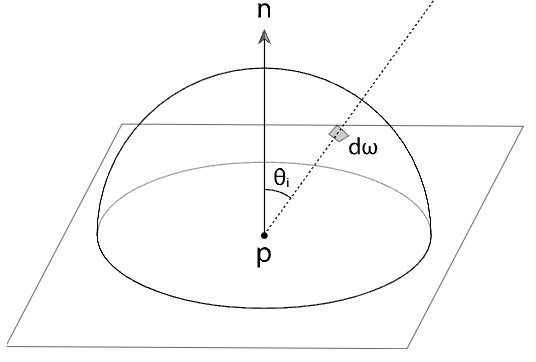
\includegraphics[scale=0.5]{./Imagens/irradiance_hemisphere.png}
        \end{center}
  \legend{ \small Fonte: \cite{pbr}. Adaptada.}
\end{figure}


\begin{figure}[h]
  \caption{\label{solid-angle} \small   Ângulo sólido s do objeto B visto pelo ponto p. }
        \begin{center}
            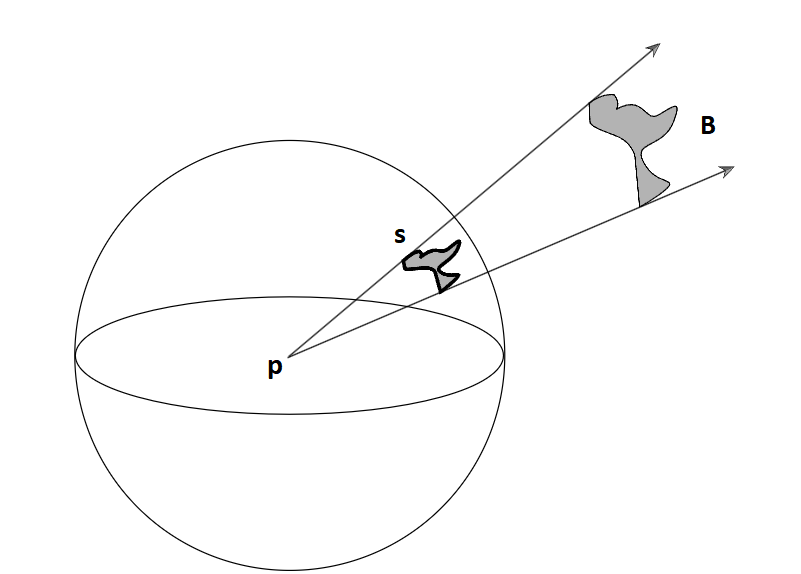
\includegraphics[scale=0.5]{./Imagens/solid_angle.png}
        \end{center}
  \legend{ \small Fonte: \cite{pbr}.}
\end{figure}




% \begin{align*} 
%   L(p,{\omega}) &= \frac{dE_{\omega}(p)}{d{\omega}} \qquad \left[\frac{J}{s\cdot m^2\cdot \text{sr}}\right]\\ 
% E_{\omega} &\text{ é função de irradiância numa direção ${\omega}$ } 
% \end{align*}


Equivalentemente, podemos definir radiância para diferentes orientações da superfície e direção do raio ao introduzir o fator $\cos(\theta)$, tal que $\theta$ é o ângulo entre a normal da superfície e a direção ${\omega}$ \cite[5.4.1]{pbr}. Essa definição é dada pela \autoref{eq-radiance-2}. 


\begin{equation} \label{eq-radiance-2}
  L(p,{\omega}) = \frac{d^2\phi(p)}{dAd{\omega} \cos(\theta)} = \frac{dE(p)}{d{\omega} \cos(\theta)} 
\end{equation}




A radiância pode fornecer informação sobre o quanto um ponto específico está iluminado na direção da câmera. Ela depende não apenas da direção do raio que incide, mas também das propriedades de refletância da superfície. E, no contexto de renderização, a radiância de uma superfície na cena se correlaciona com a irradiância de um pixel em uma imagem pela \autoref{eq-radiance-2}. Isolando o termo $E(p)$, encontramos essa relação de maneira explícita na \autoref{eq-irradiance-explicit}.


\begin{equation} \label{eq-irradiance-explicit}
  \begin{aligned}
  &E(p) = \int_{H^2}{L(p,{\omega})\cos(\theta)d{\omega}}\\
  &H^2 \text{ é o hemisfério no plano tangente à superfície no ponto $p$}
  \end{aligned}
\end{equation}




A principal funcionalidade de um renderizador fotorrealista é estimar a radiância em um ponto $p$ numa dada direção ${\omega}_o$. Essa radiância é dada pela \autoref{eq-rendering-equation}, conhecida como equação de renderização apresentada por \citeonline{rendering_equation}. Note que essa equação envolve um termo de radiância recursivo; o caso base ocorre quando não há mais o termo recursivo, isto é, a radiância é contribuída apenas por radiância emitida $L_e$, como ocorre com fontes de luz.


\begin{equation}\label{eq-rendering-equation}
\begin{aligned}
  &L_o(p, {\omega}_o) = L_e(p, {\omega}_o) + 
\int_{H^2}f(p, {\omega}_i, {\omega}_o){L_i(p,{\omega}_i)\cos(\theta_i)d{\omega}_i}\\
    &L_o \text{ é radiância de saída (\textit{outgoing})}\\
    &L_e \text{ é radiância emitida pela superfície (i.e. fonte de luz)}\\
    &L_i \text{ é radiância incidente na superfície}\\
    &{\omega}_i \text{ é a direção incidente}\\
    &{\omega}_o \text{ é a direção de saída}\\
    &H^2 \text{ são todas as direções no hemisfério no ponto $p$}\\
    &\theta_i \text{ ângulo entre direção incidente e a normal da superfície}\\
    &f \text{ função de refletância}\\
\end{aligned}
\end{equation}


A Função de Distribuição Bidirecional de Reflectância (BRDF) descreve como a luz reflete de uma superfície em diferentes direções, afetando a radiância de saída \cite{overview_brdf}. Assim, BRDFs encapsulam as propriedades de reflexão de um material, considerando fatores como a rugosidade da superfície, o ângulo de incidência e o ângulo de reflexão. Formalmente uma BRDF pode ser definida por $f({\omega}_i, {\omega}_o)$, onde ${\omega}_i$ é a direção incidente de luz e ${\omega}_o$ é a direção de saída. Para BRDFs fisicamente realistas, algumas propriedades devem ser respeitadas \cite[5.6]{pbr}:


\begin{itemize}
  \item A positividade, $f(\omega_i, \omega_o) \geq 0 $, que garante não existência de energia negativa. 


  \item A reciprocidade de Helmhotz, $f(\omega_i, \omega_o) = f(\omega_o, \omega_i)$, é o princípio que indica que a função de refletância de uma superfície permanece inalterada quando os ângulos de incidência e reflexão da luz são trocados. Isso é utilizado na otimização do traçado de raios durante a renderização, permitindo traçar os raios da câmera para a fonte de luz. Essa abordagem evita o desperdício computacional em raios que não contribuem significativamente para a intensidade de um pixel na imagem final.


  \item A conservação de energia, expressa por $\forall \omega_i, \int_{H^2}{f(\omega_i, \omega_o)cos(\theta_o) d\omega_o} \leq 1$, implica que parte da energia pode ser absorvida, transformando-se em outras formas de energia, como calor. Portanto, a soma infinitesimal pode atingir no máximo 1, mas nunca ultrapassá-la.
\end{itemize}


\section{Modelos de BRDFs } \label{brdfmodels}
As próximas seções apresentam alguns modelos comuns de BRDFs  na literatura \cite{overview_brdf}.




\subsection{BRDF Pura Especular}
Uma superfície puramente especular reflete a luz apenas em uma direção, seguindo a lei física da reflexão \cite{laws_of_refletion}, ela produz reflexões nítidas, semelhantes a espelhos. A BRDF para essa superfície é frequentemente representada pela \autoref{eq-specular}, onde $\omega_i$ é a direção da luz incidente, $\omega_o$ é a direção refletida e $\delta$ é a função delta de Dirac que garante que toda a luz incidente seja refletida na direção perfeitamente espelhada como na \autoref{specular}. Esse tipo de superfície é comum em materiais como metal polido ou vidro.


\begin{equation} \label{eq-specular}
f(\omega_i, \omega_o) = k_s \cdot \delta(\omega_i - \omega_o)
\end{equation}


\begin{figure}[H]
        \caption{\label{specular} \small Reflexão especular. Em vermelho está o raio incidente, e em azul o raio de saída.}
        \begin{center}
            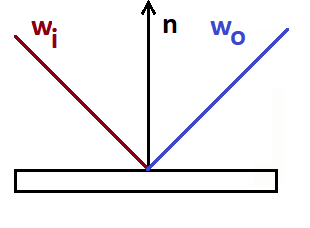
\includegraphics[scale=0.5]{./Imagens/specular-2d.png}
        \end{center}
        \legend{ \footnotesize 
  Fonte: Autor.}
\end{figure}


\subsection{BRDF Difusa Ideal}
Uma BRDF difusa ideal reflete a luz incidente uniformemente em todas as direções, sem preferência por ângulos específicos. É representada pela função $f$ na \autoref{eq-diffuse}, onde $\rho_d$ é o albedo da superfície e $\theta$ é o ângulo entre a direção da luz incidente e a normal da superfície. O termo cosseno garante que a radiância refletida seja proporcional ao cosseno do ângulo entre a direção da luz incidente e a normal da superfície, como ilustrado na \autoref{diffuse}. Esse modelo pode representar superfícies como tinta fosca ou papel.


\begin{equation} \label{eq-diffuse}
f(\omega_i, \omega_o) = \frac{\rho_d}{\pi} \cdot \cos \theta
\end{equation}


\begin{figure}[H]
        \caption{\label{diffuse} \small Reflexão Difusa. Note que os raios refletidos não dependem do ângulo de entrada.}
        \begin{center}
            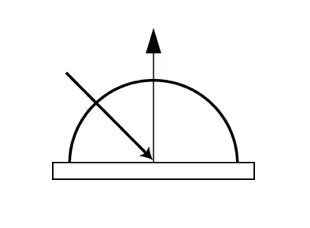
\includegraphics[scale=0.5]{./Imagens/diffuse-2d.png}
        \end{center}
        \legend{ \footnotesize Fonte: Autor. }
\end{figure}


\subsection{BRDF \textit{Glossy}}
Uma superfície pode exibir propriedades de reflexão tanto especulares quanto difusas, como na \autoref{glossy}. Uma BRDF para uma superfície brilhante é frequentemente representada por uma combinação de termos especulares e difusos, como o modelo de Blinn-Phong \cite{blinn_phong}.


\begin{figure}[H]
  \caption{\label{glossy} \small Reflexão \textit{glossy}. }
        \begin{center}
            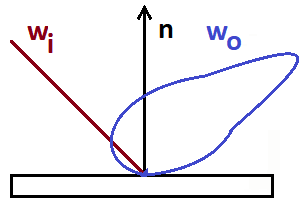
\includegraphics[scale=0.5]{./Imagens/glossy-2d.png}
        \end{center}
        \legend{\footnotesize  Fonte: Autor.}
\end{figure}




\subsection{BRDF Retro-Refletora}
Uma superfície retro-refletora reflete a luz incidente de volta na direção de onde veio, como na \autoref{retro_refletora}. A BRDF para uma superfície retro-refletora envolve tipicamente geometria especializada ou revestimentos projetados para redirecionar a luz de volta para a fonte.


\begin{figure}[H]
  \caption{\label{retro_refletora} \small Reflexão retro-refletora.}
        \begin{center}
            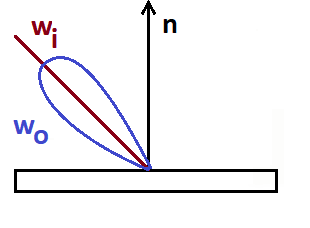
\includegraphics[scale=0.5]{./Imagens/retro-reflection-2d.png}
        \end{center}
        \legend{\footnotesize  Fonte: Autor.}
\end{figure}




\section{Introdução ao Shading e ao \textit{pipeline} de GPU} \label{shading}


\textit{Shading} refere-se ao processo de determinar a cor e o brilho dos pixels em uma imagem renderizada. Isso envolve simular a interação da luz com as superfícies, levando em consideração as propriedades dos materiais, condições de iluminação e orientação da superfície. Isso é alcançado por meio de pequenos programas chamados \textit{shaders}, que são compilados e executados na unidade de processamento gráfico (GPU).




A interação com as GPUs é facilitada por meio de uma 
API, sendo o OpenGL uma API padrão para o uso de funções na GPU \cite{opengl_spec}. O \textit{pipeline} de renderização do OpenGL é composto por várias etapas, incluindo definição de dados de vértices, \textit{shaders} de vértice e fragmento, \textit{shaders} de tesselação e geometria opcionais, configuração de primitivas, recorte e rasterização.


% Essas etapas coordenam o fluxo de dados da CPU para a GPU e suas transformações, culminando na geração da imagem final. As etapas mais importantes para o nosso trabalho são os \textit{shaders} de fragmento e de vértice, representados na \autoref{fig-pipeline}, os quais executam a manipulação dos vértices e determinam cores de pixels, respectivamente.


Essas etapas coordenam o fluxo de dados da CPU para a GPU e suas transformações, culminando na geração da imagem final. Uma representação visual desse processo pode ser observada na \autoref{fig-pipeline}. Nela, é representado a CPU enviando os dados da cena para a GPU, que utiliza essas informações nos \textit{shaders} de vértice e fragmento. O \textit{shader} de vértice manipula os vértices da cena, enquanto o \textit{shader} de fragmento determina as cores dos pixels. Os fragmentos são elementos gerados durante o processamento das primitivas geométricas, como triângulos. Eles correspondem a pontos discretos na tela onde a cor final será determinada. Além disso, a CPU também pode enviar variáveis uniformes (\textit{uniform variables}) para os \textit{shaders}, que são essenciais para a etapa de renderização e contribuem para a geração da imagem final.


\begin{figure}[H]
        \caption{\label{fig-pipeline}\small O \textit{pipeline}.}
        \begin{center}
            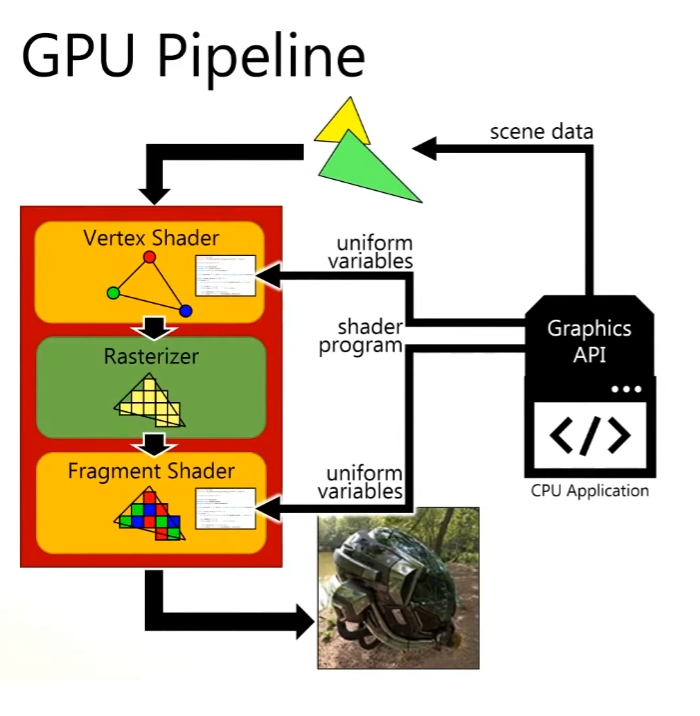
\includegraphics[scale=0.45]{./Imagens/gpu_pipeline.png}
        \end{center}
  \legend{Fonte: \cite{video_pipeline}.}
\end{figure}




\subsection{Shader de Vértice}


O \textit{shader} de vértice opera em vértices individuais de primitivas geométricas antes de serem rasterizados em fragmentos. Sua principal tarefa é transformar vértices e passar os dados necessários para o \textit{shader} de fragmentos. Esses \textit{shaders} geralmente realizam várias transformações nos dados dos vértices, permitindo que objetos sejam posicionados, orientados e projetados em uma tela bidimensional (2D). Um exemplo desse \textit{shader} está no \autoref{vertex_code1}, que usa uma matriz para realizar essas transformações. Ao fim dessa etapa, os vértices são normalizados para coordenadas homogêneas. Essa normalização é essencial para realizar a projeção perspectiva e outros cálculos no \textit{pipeline} de renderização.




\begin{codigo}[H]
  \caption{\small Exemplo GLSL de \textit{shader} de vértice.}
 \label{vertex_code1}
\begin{lstlisting}
#version 330 core
layout(location = 0) in vec3 inPosition;
layout(location = 1) in vec3 inNormal;


uniform mat4 modelViewProjection;


out vec3 fragNormal;


void main() {
    vec3 manipulatedPosition = inPosition + (sin(gl_VertexID * 0.1) * 0.1);
    fragNormal = inNormal;
    gl_Position = modelViewProjection * vec4(manipulatedPosition, 1.0);
}
\end{lstlisting}
\end{codigo}


\subsection{Shader de Fragmento}


O \textit{shader} de fragmento opera sobre os fragmentos produzidos pela etapa de rasterização. Sua principal responsabilidade é determinar a cor final de cada fragmento com base na iluminação, texturização e propriedades da superfície. Uma possível interpretação é que esse programa é repetido para todos os pixels da imagem paralelamente.  Ele recebe dados interpolados, como vértices e normais, ou seja, cada instância desse programa possui entradas potencialmente diferentes uma das outras. Na API OpenGL, valores como normais e vértices são interpolados usando coordenadas baricêntricas \cite{opengl_interpolation}.


As BRDFs podem ser implementadas nesse estágio do \textit{pipeline} para atingir um nível de \textit{shading} mais preciso, pois é possível ter mais dados do que os definidos na geometria devido à interpolação. Isso resulta em um nível de detalhamento potencialmente maior, considerando uma transição mais suave de um ponto para outro dentro de um triângulo,  como representado na \autoref{better-with-fragment}.




\begin{figure}[H]
        \caption{\label{better-with-fragment} \small Diferença entre shading a nível de vértice e shading a nível de fragmento.}
        \begin{center}
            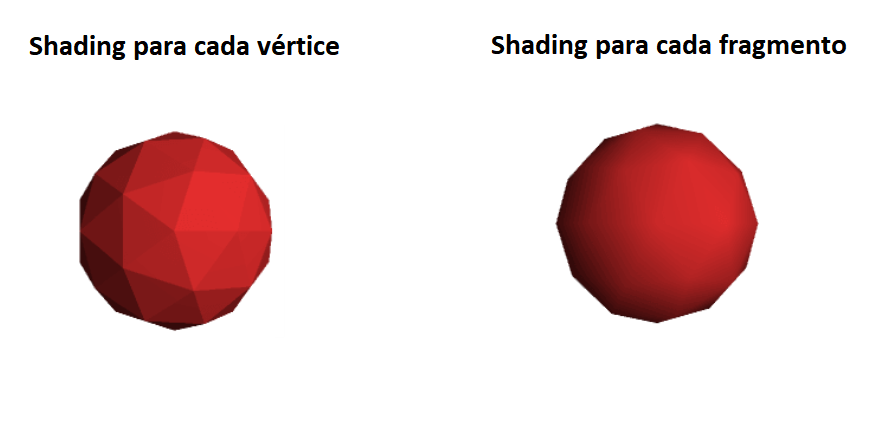
\includegraphics[scale=0.5]{./Imagens/per_vertex_per_frag.png}
        \end{center}
  \legend{ Fonte: \cite{pervertex_perfrag}.}
\end{figure}


\section{Compiladores} \label{compiladores}


\subsection{Cadeia de Símbolos e Alfabeto} \label{símbolos}


Um \textbf{cadeia de símbolos} é uma sequência finita de símbolos retirados de um alfabeto $ \Sigma $. Formalmente, uma cadeia $ w $ é representada como $ [w_1, w_2, ..., w_n] $, onde cada $ w_i $ pertence ao alfabeto $ \Sigma $. O \textbf{alfabeto} $ \Sigma $ é um conjunto finito de símbolos distintos usados para construir cadeias em uma linguagem. Ele define os blocos de construção a partir dos quais cadeias válidas na linguagem são formadas.


\subsection{Definições de Linguagens} \label{linguagem}


Na ciência da computação, as linguagens são sistemas formais compostos por símbolos e regras que são muito úteis para definir um significado algorítmico. Uma \textbf{linguagem} $L$ é definida como um conjunto de cadeias sobre um alfabeto finito $ \Sigma $, $ L \subseteq \Sigma^* $, onde  $ \Sigma^* $ denota o conjunto de todas as cadeias possíveis sobre $ \Sigma $ \cite{language_theory}. A estrutura semântica de uma linguagem inclui seu alfabeto $ \Sigma $, sintaxe e regras de gramática.


\subsection{Compilador como um Transformação}


Um compilador pode ser visto como uma transformação entre linguagens $ L_1 $ e $ L_2 $ que preserva a estrutura interna dos conjuntos, isto é, deve manter o mesmo significado algorítmico. Assim, o compilador $ C: L_1 \rightarrow L_2 $ mapeia programas escritos na linguagem de origem $ L_1 $ para programas equivalentes na linguagem de destino $ L_2 $. Essa transformação garante a preservação semântica, mantendo o comportamento pretendido do programa original durante a tradução.




\subsection{Gramática} \label{gramatica}


Durante a criação de um compilador, é necessário entender as regras que auxiliam na validação da linguagem de entrada, essas regras podem ser formalizadas pela gramática. Uma gramática $G$ é um sistema formal composto por um conjunto de regras de produção que especificam como cadeias válidas na linguagem podem ser geradas \cite{language_theory}. Ela inclui terminais, não-terminais, regras de produção e um símbolo inicial.


\begin{itemize}
  \item Terminais: são os símbolos básicos a partir dos quais as cadeias são formadas. Eles representam as unidades elementares da sintaxe da linguagem.
  \item Não-terminais: são espaços reservados que podem ser substituídos por terminais ou outros não-terminais de acordo com as regras de produção.


  \item Regras de Produção: definem a transformação ou substituição de não-terminais em sequências de terminais e/ou não-terminais.


  \item Símbolo Inicial: é um não-terminal especial a partir do qual a derivação de cadeias válidas na linguagem começa.
\end{itemize}




\subsubsection{Gramáticas Livres de Contexto (GLCs)}


Um tipo comum de gramática usado na definição de linguagens é a gramática livre de contexto (GLC).  Uma GLC pode ser descrita formalmente como $ G=(V,\Sigma,R,S)$:


\begin{itemize}
  \item $V$ é um conjunto finito de símbolos não-terminais.


  \item $\Sigma$ é um conjunto finito de símbolos terminais disjunto de $V$.


  \item $R$ é um conjunto finito de regras de produção, cada regra no formato $A \rightarrow \beta$, onde $A$ é um não-terminal e $\beta$ é uma cadeia de terminais e não-terminais.


  \item $S$ é o símbolo inicial, que pertence a $V$.
\end{itemize}


O processo de gerar uma cadeia na linguagem definida por uma gramática é chamado de derivação. Isso envolve aplicar regras de produção sucessivamente, começando pelo símbolo inicial $S$ até restarem apenas símbolos terminais.


Uma árvore sintática é uma representação gráfica do processo de derivação, onde cada nó representa um símbolo na cadeia. As arestas representam a aplicação de regras de produção. Em código, essa árvore é gerada e usada como representação intermediária,  auxiliando na geração da linguagem alvo $L_2$.




\subsection{Análise Léxica}
A análise léxica, também conhecida como \textit{lexing} ou \textit{tokenization}, é a primeira etapa do processo de compilação, na qual a entrada textual é dividida em unidades léxicas significativas chamadas de \textit{tokens}. Esses \textit{tokens} representam os componentes básicos da linguagem, como palavras-chave, identificadores, operadores e literais. O analisador léxico percorre o código-fonte caractere por caractere, agrupando-os em \textit{tokens} conforme regras pré-definidas pela gramática da linguagem. Essa linguagem é, geralmente, reconhecível por máquinas de estado \cite{automata}.


\subsection{Análise Sintática ou \textit{Parsing}}
A análise sintática é a segunda fase do processo de compilação, na qual os \textit{tokens} gerados pela análise léxica são organizados e verificados quanto à conformidade com a gramática da linguagem. Essa etapa envolve a construção de uma árvore sintática, ou estrutura de dados equivalente, que representa a estrutura hierárquica das expressões e instruções do programa. O analisador sintático utiliza regras de produção gramatical para validar a sintaxe do código-fonte e identificar possíveis erros.


\subsubsection{Pratt Parsing}
O Pratt \textit{Parsing}, introduzido por Vaughan Pratt, é uma técnica de análise sintática recursiva que permite analisar expressões com precedência de operadores de forma eficiente e sem ambiguidades \cite{pratt}. Uma das suas características distintivas é determinar a ordem de avaliação das expressões. Ao contrário da análise descendente recursiva tradicional, na qual cada não-terminal possui uma função de \textit{parsing}, a análise Pratt associa funções de manipulação (\textit{handlers}) com \textit{tokens}.


A precedência das expressões é definida por meio de uma tabela, na qual cada operador é associado a um valor que permita o \textit{parser} decidir dinamicamente a ordem de avaliação das expressões com base nos operadores encontrados durante a análise. Essa abordagem simplifica significativamente a implementação do \textit{parser} e elimina a necessidade de criar uma gramática que encapsula a precedência em sua definição. Ela também evita a recursão profunda para lidar com diferentes níveis de precedência.


% \subsubsection{Árvores Inclinadas}
%
% Em uma árvore inclinada à direita, operadores com maior precedência são resolvidos primeiro, mesmo que apareçam na direita da expressão. Isso resulta em uma árvore onde os operadores com maior precedência estão mais próximos da raiz, indicando que eles são avaliados primeiro. Considere a expressão ``1 + 2 * 3'', apesar de ``*'' aparecer após ``+'',  ``*'' tem uma precedência mais alta e, portanto, forma uma subárvore que é resolvida antes da adição.
%
%
% \begin{verbatim}
%                +
%               / \
%              1   *
%                 / \
%                2   3
% \end{verbatim}
%
% Por outro lado, em uma árvore inclinada à esquerda, operadores com maior precedência são resolvidos por último, seguindo uma ordem de avaliação da esquerda para a direita. As árvores inclinadas à esquerda estão tipicamente associadas a chamadas recursivas de \textit{parsing}, já as inclinadas à direita estão associadas a iteração. Para alcançar a estrutura correta da árvore, o Pratt \textit{parsing} alterna entre recursão e iteração com base na precedência dos operadores para saber o momento de gerar uma subárvore inclinada para esquerda ou direita.


\subsubsection{Pseudo-código para Análise de Expressões}


O pseudo-código \ref{alg1}
demonstra o Pratt \textit{parsing} para a construção de árvores de expressão. Esse algoritmo também é robusto mesmo quando um operador é tanto infixo quanto prefixo, por exemplo ``$-$'' pode ser um \textit{token} de subtração ou de negação. Assim, cada \textit{token} tem uma função de prefixo e infixo associada.


Nesse algoritmo, 
\textbf{proximo\_token()} recupera o próximo elemento da lista de \textit{tokens},
\textbf{token.precedencia}() retorna a procedência do token atual, \textbf{token.prefixo()} é a função associada ao \textit{token} que faz o \textit{parsing} de uma expressão quando o \textit{token} é o primeiro símbolo em uma subexpressão (e.g. o token ``$-$'' é o primeiro na expressão ``$-3$''). Enquanto o \textbf{token.infixo(esquerda)} é a função associada ao \textit{token} que utiliza outra subárvore já criada como entrada. Por exemplo a subárvore \textbf{esquerda} pode ser a expressão ``$-3$'', o \textit{token} atual ser ``$*$'' e o retorno gera a expressão completa ``$-3 * 1$''.


Tanto \textbf{token.infixo} quanto \textbf{token.prefixo} podem ser indiretamente recursivas, isto é, ambas podem chamar a função \textbf{expressão} no \autoref{alg1}. 
Por fim, \textbf{precedencia\_anterior} representa a precedência do \textit{token} anterior.


\begin{algoritmo}[H]
        \caption{\small Função Pratt Parsing de Expressão.}
        \label{alg1}
  \begin{lstlisting}
  function expressao(precedencia_anterior:=0):
      token := proximo_token()
      esquerda := token.prefixo()
      while precedencia_anterior < token.precedencia():
          token    = proximo_token()
          esquerda = token.infixo(esquerda)
      return esquerda
  \end{lstlisting}
\end{algoritmo}


\subsection{Análise Semântica}


A análise semântica é uma etapa essencial no processo de compilação, responsável por garantir a corretude semântica das declarações e instruções do programa. Durante essa fase, são aplicadas verificações para garantir que as operações sejam realizadas com tipos compatíveis.


Um exemplo típico de verificação semântica é a inferência de tipos em expressões. Por exemplo, no \autoref{cod-exemplo-c} o analisador semântico infere que o número inteiro $30$ deve ser convertido para o tipo \textit{float} antes da multiplicação, garantindo consistência de tipos. Além da verificação de tipos, o analisador semântico identifica e reporta outros erros comuns, como variáveis não declaradas e falhas no controle de fluxo do programa.


\begin{codigo}
\caption{\small Exemplo de código escrito em C.}
  \label{cod-exemplo-c}
\begin{lstlisting}[language=C]
float x = 10.1;
float y = x * 30;
\end{lstlisting}
\end{codigo}



No contexto deste trabalho, a análise semântica é importante para validar expressões e funções relacionadas à renderização de materiais no desenvolvimento de \textit{shaders} no OpenGL. Por exemplo, ao escrever uma função BRDF em GLSL, o analisador deve verificar se os tipos de dados e operações são compatíveis tanto com a definição da função BRDF quanto com as dimensões de vetores e outras grandezas definidas.


\subsection{Geração da Linguagem Alvo} \label{codegen}


Nesta fase, fazemos a transição da representação intermediária  da linguagem origem \( L_1 \)  para  a linguagem de destino \( L_2 \), processo que envolve traduzir construções de \( L_1 \) para equivalentes em $L_2$. Podemos realizar essa tradução ao percorrer recursivamente os nós da árvore sintática usando as informações contidas nesses nós para gerar partes do programa final em $L_2$.


Dado um programa $a \in L_1$ existem vários programas $b_{i=1,2,3,...} \in L_2$ que possui estrutura semanticamente equivalentes à $a$. Ao explorar esse conjunto, é possível escolher um $b_j \in L_2$ tal que esse programa seja otimizado em algum sentido, como uso eficiente de memória ou executar menos instruções de \textit{hardware}. Nosso foco neste trabalho está na tradução semanticamente correta, sem envolver exploração das saídas  equivalentes.


Como exemplo, considere a tradução de um cálculo matemático de \( L_1 \) (\LaTeX{}), para \( L_2 \) (GLSL). O cálculo apresentado na \autoref{eq-calculo-vetorial} pertence a $L_1$. O \autoref{cod-fonte-calculo} mostra o código-fonte desse cálculo. 




\begin{equation} \label{eq-calculo-vetorial}
 \quad \mathbf{v} = (\mathbf{a} + \mathbf{b}) \cdot
 \mathbf{c} - (\mathbf{d} \times \mathbf{e})
\end{equation}


\begin{codigo}
  \caption{\small Cálculo vetorial em código-fonte \LaTeX{}.}
  \label{cod-fonte-calculo}
\begin{lstlisting}
 \mathbf{v} = (\mathbf{a} + \mathbf{b}) \cdot
 \mathbf{c} - (\mathbf{d} \times \mathbf{e})
\end{lstlisting}
\end{codigo}






Após a tradução da expressão matemática para \( L_2 \), o cálculo pode ser convertido para o trecho de programa apresentado no \autoref{cod-calculo-vetorial-glsl}. Esse código é válido na linguagem GLSL.


\begin{codigo}
\caption{\small Cálculo vetorial em código GLSL.}
\label{cod-calculo-vetorial-glsl}
\begin{lstlisting}[language = C]
    vec3 v = dot(a + b, c) - cross(d, e);
\end{lstlisting}
\end{codigo}




\chapter{Revisão Bibliográfica} \label{revisao}


Para esta seção, será conduzida uma revisão literária abrangente com o objetivo de explorar trabalhos relacionados ao desenvolvimento de compiladores para tradução de BRDFs expressas em \LaTeX{} para a linguagem de \textit{shading}, empregando técnicas de \textit{parsing}. O processo de busca será conduzido em duas etapas distintas. Inicialmente, será realizado um levantamento dos trabalhos existentes nas bases de dados  com relevantes periódicos, anais de eventos, artigos e trabalhos. Por fim, será realizada uma busca por produtos ou ferramentas similares no mercado, utilizando \textit{strings} de busca específicas em repositórios digitais, especificamente GitHub e SourceForge. Esses processos de busca permitirão identificar referências relevantes e estabelecer um panorama do estado da arte no campo dos compiladores de BRDFs  para \textit{shaders}, contribuindo para a compreensão do contexto acadêmico e prático no qual este trabalho se insere.


\section{Mapeamento Sistemático}


Com o intuito de obter resultados relevantes para a pesquisa, foram elaboradas frases de busca com base nos termos-chave relacionados ao tema deste trabalho. Também foram criadas questões de pesquisa para guiar a seleção dos trabalhos.


\subsection{Seleção das Bases}
As bases escolhidas foram: ACM Digital Library \footnote{\url{https://dl.acm.org/}},  IEEE Xplorer Digital Library \footnote{\url{https://ieeexplore.ieee.org/}},  Biblioteca Digital Brasileira de Teses e Dissertações (BDTD) \footnote{\url{https://bdtd.ibict.br/}}, Portal de Periódicos da CAPES \footnote{\url{https://www-periodicos-capes-gov-br.ezl.periodicos.capes.gov.br/index.php?}},  Google Acadêmico \footnote{\url{https://scholar.google.com/}}. Essas foram escolhidas por serem acessíveis gratuitamente pela afiliação à Universidade Federal de Sergipe, já o Google Scholar foi escolhido por agregar pesquisas em outras bases que possam ter trabalhos relevantes.


% 
%


%
% \url{https://www-periodicos-capes-gov-br.ezl.periodicos.capes.gov.br/}








\subsection{Questões de Pequisa}  \label{questoes-pesquisa}


Foram elaboradas questões de pesquisa específicas, que guiam as frases-chave que refletem os principais aspectos do tema em questão. A partir desse processo, foram identificados e selecionados os trabalhos que melhor atendiam às questões propostas, garantindo maior relevância para este estudo.


\begin{enumerate}
  \item Quais são as abordagens mais comuns utilizadas na criação de compiladores para tradução de BRDFs expressas em alguma linguagem de texto, como \LaTeX{}, para \textit{shaders}?


  \item Quais as técnicas de \textit{parsing} têm sido aplicadas no desenvolvimento de compiladores para linguagens matemáticas?


  \item O trabalho utiliza árvores ou gramáticas livres de contexto para representar uma BRDF?


 \item Quais são os principais desafios enfrentados ao traduzir funções matemáticas complexas, como as BRDFs, em \textit{shaders}?


 \item Quais são as ferramentas e recursos disponíveis para auxiliar no desenvolvimento de compiladores para BRDFs e \textit{shaders}, e como eles podem ser integrados ao processo de desenvolvimento?


\end{enumerate}






\subsection{Termos de Busca}
 As frases foram construídas considerando suas variações equivalentes através de operadores lógicos. Posteriormente, as frases de pesquisa foram adaptadas de acordo com as características individuais de cada base de dados utilizada. Os termos-chave escolhidos foram: ("shader" AND "BRDF" AND ("compiler"\ OR "parser"\ OR "grammar")), conforme demonstrado na \autoref{tab-bases}.




\begin{table}[H]
\ABNTEXfontereduzida
\caption[bases]{\small Tabela de pesquisa.}
\label{tab-bases}
\begin{tabular}{p{2.6cm}|p{6.0cm}|p{2.25cm}|p{3.40cm}}
  %\hline
   \textbf{Bases} & \textbf{Termos de Pesquisa}  & \textbf{Resultados}\\
   \hline
    IEEE Xplore Digital Library
    &
    ("Full Text \& Metadata":brdf)
AND (("Full Text \& Metadata":shader) OR  ("Full Text \& Metadata":shading))
AND (("Full Text \& Metadata":compiler) OR  ("Full Text \& Metadata":parsing) OR  ("Full Text \& Metadata":parser) OR  ("Full Text \& Metadata":grammar))
   & 36
    \\ \hline


    BDTD
    & (Todos os campos:compiler OU Todos os campos:parsing OU Todos os campos:parser OU Todos os campos:compilador) E (Todos os campos:shader OU Todos os campos:shading) E (Todos os campos:brdf)
    & 0
    \\ \hline
    CAPES Periódico
    &  Qualquer campo contém brdf E 
 Qualquer campo contém compi* E shad*  
    & 0
    \\ \hline


  ACM Digital Library
  & AllField:((shader OR shading) AND brdf AND (compiler OR compiling) AND (parser OR grammar OR parsing))
  & 46
    \\ \hline


 Google Acadêmico 
  & 
  ("BRDF" AND ("COMPILER" OR "COMPILING") AND( "PARSER" OR "PARSING") AND ("SHADER" OR "SHADING"))
  & 69
   % \hline
\end{tabular}
\end{table}


\subsection{Critérios}


Para garantir a relevância dos resultados obtidos, seguimos os critérios de inclusão e exclusão estabelecidos, de forma a filtrar os resultados. Ao fim desse procedimento, apenas os resultados com maior compatibilidade com este trabalho foram analisados e descritos de maneira detalhada. O resultados se encontram na \autoref{tab-result}.


\subsubsection{Critérios de Inclusão}


\begin{enumerate}
  \item Foram incluídos artigos relacionados às palavras-chaves;
  \item Foram incluídos artigos que de alguma forma citem a criação de um compilador ou um \textit{parser};
  \item Foram incluídos artigos que sintetizam uma árvore como representação de BRDFs.
\end{enumerate}


\subsubsection{Critérios de Exclusão}


\begin{enumerate}
  \item Foram excluídos artigos que dispunham de \textit{links} incorretos e ou quebrados;
  \item Foram excluídos artigos no quais os projetos são muito similares;
  \item Foram excluídos artigos que não respondem as questões de pesquisa na \autoref{questoes-pesquisa};
  \item Foram excluídos artigos que não têm como entrada uma BRDF no formato de equação, ou seja, utilizam a representação diretamente como código;
  \item Foram excluídos artigos que não consideram a geração de \textit{shaders} como saída ou estrutura da BRDF em árvore;
  \item Foram excluídos artigos que não citam BRDFs e compilador ou árvores em seu resumo;
  \item Se, após a leitura completa, o artigo não concerne os interesses deste trabalho, esse foi excluído.
\end{enumerate}




\begin{table}[H]
\ABNTEXfontereduzida
  \caption[bases]{\small Resultados das bases após aplicar os critérios.}
\label{tab-result}
\begin{tabular}{p{6.6cm}|p{6.6cm}}
  %\hline
   \textbf{Bases}  & \textbf{Filtrados}\\
   \hline
    IEEE Xplore Digital Library
   & 2
    \\ \hline
    BDTD
    & 0
    \\ \hline
    CAPES Periódico
    & 0
    \\ \hline


  ACM Digital Library
  & 1
    \\ \hline
 Google Acadêmico 
  & 1
   % \hline
\end{tabular}
\end{table}






\subsection{Descrição dos Trabalhos Relacionados}


\subsubsection{genBRDF: Discovering New Analytic BRDFs with Genetic Programming}


Neste artigo é introduzido uma  \textit{framework} chamada genBRDF, a qual aplica técnicas de programação genética para explorar e descobrir novas BRDFs de maneira analítica \cite{genbrdf}. O processo inicia utilizando uma BRDF existente, e interativamente aplica mutações e recombinações de partes das expressões matemáticas que compõem essas BRDFs à medida que novas gerações surgem. Essas mutações são guiadas por uma função \textit{fitness}, que seria o inverso de uma função de erro, elas são baseadas em um \textit{dataset} de materiais já medidos. Por meio da avaliação de milhares de expressões, a  \textit{framework} identifica as viáveis.


Os autores geraram uma gramática que inclui constantes e operadores matemáticos comuns encontrados em equações BRDF. A gramática é compilada, e a árvore de sintaxe abstrata resultante passa por modificações realizadas pelo algoritmo genético. Nós na árvore podem ser trocados, substituídos, removidos e novos nós podem ser adicionados. Esse processo, após refinamento e análise, resulta em novas BRDFs. Alguns dos novos modelos BRDF apresentados no documento incluem aqueles que superam os modelos existentes em termos de precisão e simplicidade.
 
Esse artigo se concentra em automaticamente encontrar novos modelos analíticos de BRDF, em vez de compilar diretamente equações BRDF em linguagens de \textit{shading}. Embora a representação das expressões das BRDFs possa potencialmente inspirar o nosso trabalho, o principal objetivo do artigo difere do nosso tema.


\subsubsection{Slang: language mechanisms for extensible real-time shading systems}


O artigo descreve a linguagem \texttt{Slang}, uma extensão da amplamente utilizada linguagem de \textit{shading} HLSL, projetada para melhorar o suporte à modularidade e extensibilidade \cite{slang}. A abordagem de \textit{design} da \texttt{Slang} é baseada em dois princípios fundamentais: manter a compatibilidade com o HLSL existente sempre que possível e introduzir recursos com precedentes em linguagens de programação \textit{mainstream} para facilitar a familiaridade e intuição dos desenvolvedores.


O autor enfatiza que cada extensão da \texttt{Slang} busca oferecer uma progressão incremental para a adoção a partir do código HLSL existente, eliminando a necessidade de uma migração completa. Algumas dessas extensões incluem: funções genéricas, estruturas genéricas e tipos que implementam interfaces específicas, semelhantes ao funcionamento das interfaces em \texttt{Java}, mas aplicadas a estruturas. Um exemplo de função genérica escrita em \texttt{Slang} é:


\begin{verbatim}
float3 integrateSingleRay<B:IBxDF>(B bxdf,
SurfaceGeometry geom, float3 wi, float3 wo, float3 Li)
{ return bxdf.eval(wo, wi) * Li * max(0, dot(wi, geom.n)); }


\end{verbatim}




Enquanto o artigo tenta melhorar a eficiência e a extensibilidade dos sistemas de \textit{shading} em tempo real, o nosso trabalho se concentra na compilação de equações BRDF em linguagens de \textit{shading}. Embora ambos os projetos façam uso de \textit{shaders} e compilação, as abordagens e focos são diferentes.


\subsubsection{Tree-Structured Shading Decomposition}


Esse trabalho propõe uma abordagem para inferir uma representação de BRDF estruturada em árvore a partir de uma única imagem para o sombreamento de objetos \cite{tree_decomposition}. Em vez de usar representações paramétricas, como é comum, é proposta uma abordagem que utiliza uma representação em árvore de \textit{shading}, combinando nós básicos e métodos para decompor o \textit{shading} da superfície do objeto, representado na \autoref{fig_decomp}.


\begin{figure}[H]
        \caption{\label{fig_decomp} \small Exemplo de decomposição de BRDFs em nós de uma árvore.}
        \begin{center}
            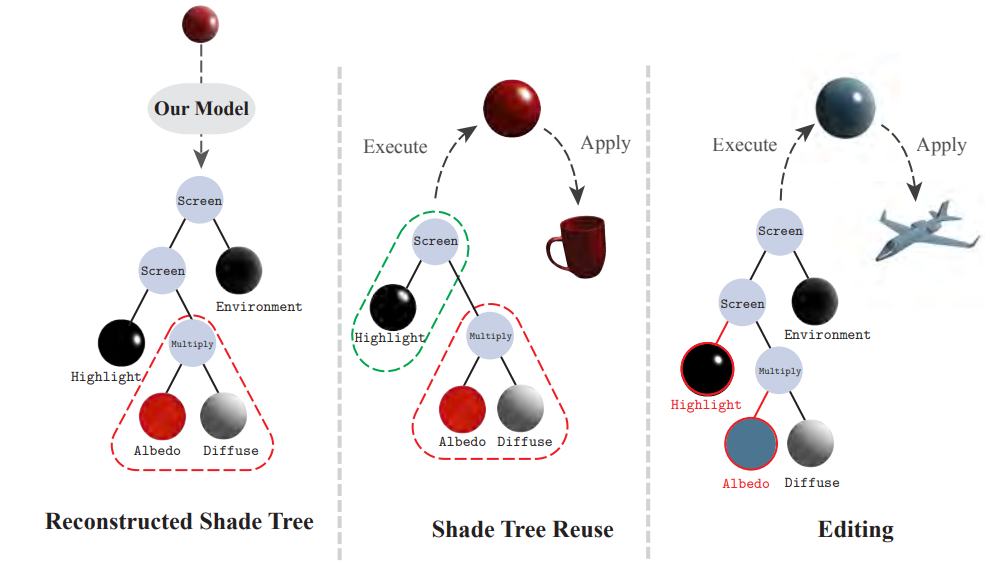
\includegraphics[scale=0.5]{./Imagens/tree-shading.png}
        \end{center}
        \legend{Fonte: \citeonline[]{radiometry_introduction}.}
\end{figure}




Assim como o nosso trabalho, esse artigo se concentra em facilitar o processo para usuários inexperientes, pois ambos visam fornecer ferramentas acessíveis para manipular representações de \textit{shading} sem exigir conhecimento avançado em programação. Esse artigo também emprega uma representação em árvore, embora para um propósito diferente.


\subsubsection{A Real-Time Configurable Shader Based on Lookup Tables}


Esse trabalho propõe uma arquitetura de \textit{hardware} que permite cálculos de \textit{shading} por pixel em tempo real, utilizando \textit{lookup-tables} \cite{configurable}. Para isso, são projetados circuitos configuráveis baseados nessas tabelas, memórias de acesso aleatório (RAMs) e memórias somente leitura (ROMs). Vários circuitos base foram projetados para as operações mais comuns. Por exemplo, circuitos para calcular o produto interno entre dois vetores e circuitos de rotação de um vetor por um ângulo, um exemplo desses diagramas é representado na \autoref{fig_circuit}. Ademais, foi utilizada interpolação em um sistema de coordenadas polares em vez da interpolação vetorial convencional, com o objetivo de reduzir o tamanho dos circuitos e melhorar o desempenho.




\begin{figure}[H]
        \caption{\label{fig_circuit}\small Exemplo de circuito de produto interno entre vetores.}
        \begin{center}
            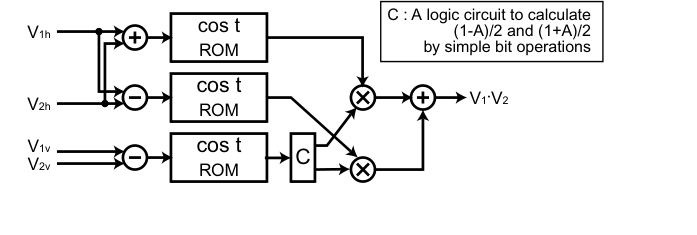
\includegraphics[scale=0.7]{./Imagens/rom-cos-lookup-table.png}
        \end{center}
  \legend{\small Fonte: \cite{configurable}.}
\end{figure}




Além disso, o circuito suporta diversas BRDFs, como Blinn-Phong, Cook-Torrance, Ward e modelos baseados em microfacetas, com tabelas específicas para cada modelo. O uso de tabelas de pesquisa permite a representação organizada da parametrização das BRDFs, tornando o processo de transformação de BRDF para \textit{shaders} mais acessível. Esse trabalho foi aceito por incluir o processo de tradução estruturada de BRDFs para os circuitos. Assim como as árvores, eles são hierárquicos e são usados em composição para representar uma BRDF. Similar a este trabalho, a abordagem facilita a geração de \textit{shaders} a partir da descrição de BRDFs, apesar da metodologia ser diferente.


\section{Pesquisa por Repositórios Online}
Também foram analisados repositórios no GitHub e SourceForge, cada um com uma \textit{string} de busca específica. Os repositórios encontrados foram filtrados baseados em seus resumos. Caso não haja a menção da criação de um compilador ou não seja citada uma transformação de BRDF para outra estrutura, esse repositório foi excluído. O resultado se encontra na \autoref{tab-repo}.




% @IMPORTANT 'preciso incluir o trabalho de conclusão de tulasi, que tem um repositório associado. Você pode colocar em uma seção diferente aqui neste capítulo. também é importante mencionar no capítulo 1 que esse trabalho existe, e que a abordagem do seu difere nas técnicas usadas.


\begin{table}[H]
\ABNTEXfontereduzida
\caption[bases]{\small Resultados da pesquisa nos repositórios.}
\label{tab-repo}
\begin{tabular}{p{2.6cm}|p{6.0cm}|p{2.25cm}|p{3.40cm}}
  %\hline
   \textbf{Plataformas} & \textbf{Termos de Pesquisa}  & \textbf{Resultados}\\
   \hline
   GitHub
   &
   in:readme (GLSL AND BRDF AND  (compiler OR compilation) AND (shader OR shading))
   & 15
   \\ \hline
   SourceForge
   &
   compiler bdrf
   & 0
\end{tabular}
\end{table}




Após ler por completo os resumos dos repositórios do GitHub, é evidente que nenhum desses projetos é relacionado com o proposto neste trabalho. Apesar de comentarem sobre BRDFs, esses projetos não implementam compiladores, não fazem \textit{parsing} de equações de BRDFs e nem mesmo geram \textit{shaders} a partir de BRDFs.


% \end{adjustwidth}

\chapter{Metodologia} \label{metodologia}

A metodologia para o desenvolvimento do compilador proposto adota uma abordagem prática, estruturada em etapas principais: a análise de informações relevantes sobre BRDFs e a compilação de \textit{shaders}; a exploração de técnicas existentes no domínio; a especificação da linguagem de entrada, um subconjunto de \LaTeX{}; a implementação do compilador; e a avaliação de seu desempenho por meio de experimentos de renderização.

Inicialmente, o método para realizar a análise e a exploração de técnicas é descrito na \autoref{analise}. Em seguida, a especificação da linguagem de entrada e saída é apresentada na \autoref{especificacao-linguagem}. É importante destacar que a definição precisa da gramática está consolidada no capítulo de desenvolvimento, na \autoref{section-parser}.

Posteriormente, é discutida a elaboração dos casos de teste para validar a correção e a precisão do compilador, conforme detalhado na \autoref{testes}. Embora o método escolhido se baseie nesses testes iniciais, os resultados obtidos no \autoref{chapter.resultados} expandem a validação para um conjunto maior de BRDFs.

O método de implementação do compilador é detalhado na \autoref{compiladorimplementacao}, enquanto a avaliação dos experimentos de renderização, focada na qualidade visual dos \textit{shaders} compilados, é abordada na \autoref{experimentos-renderizacao}.

% A \autoref{experimentos-renderizacao} planeja o método de avaliação dos experimentos de renderização quanto a qualidade visual dos \textit{shaders} compilados.

Seguindo essa metodologia, a ferramenta proposta busca compilar descrições de BRDFs em \textit{shaders} GLSL, garantindo qualidade e precisão no resultado final.

% Posteriormente, uma ideia de como o \textit{design} dos casos de teste devem ser elaborados para validar a correção e precisão do compilador é apresentado na \autoref{testes}, apesar do metódo escolhido foi os testes que mostrando, os resultados expandem esses testes e testamos mais brdfs ainda no \autoref{chapter.resultado}. O método de implementação do compilador é detalhado na \autoref{compiladorimplementacao}. Seguindo essa metodologia, a ferramenta proposta visa compilar efetivamente descrições de BRDF em \textit{shaders} GLSL.



\section{Análise e Técnicas} \label{analise}


O primeiro passo envolve a realização de uma análise detalhada das áreas relacionadas ao desenvolvimento da ferramenta proposta. Isso inclui a revisão da literatura (\autoref{revisao}) sobre BRDFs, linguagens de \textit{shaders}, \textit{design} de compiladores e técnicas de renderização gráfica. Além disso, envolve o estudo de ferramentas e bibliotecas pertinentes.

Durante essa análise, foram estudados conceitos de radiometria para compreender tecnicamente as BRDFs. A principal fonte de informação sobre radiância e BRDFs foi o livro ``Physically Based Rendering: From Theory To Implementation'' \cite{pbr}. Esse livro foi importante para compreensão da equação de renderização (\autoref{eq-rendering-equation}).

A leitura de exemplos práticos e leitura das código fonte da ferramente \autoref{fig-disney-tool} permitiu a familiarização com o desenvolvimento de BRDFs, fornecendo uma base sólida para a compreensão do mapeamento da equação para código, aspecto fundamental para o desenvolvimento do compilador proposto neste trabalho.

Ademais, foram exploradas diversas técnicas para compilação, como o método de Pratt \textit{Parsing} para a construção de um compilador, somado ao uso do conhecimento de recursividade e caminhada em arvóres para realizar a análise semantica e geração de código.


\section{Especificação da Linguagem}\label{especificacao-linguagem}

As especificações da linguagem de entrada e saída para o compilador são definidas. A linguagem de entrada é uma versão simplificada do \LaTeX{}, na qual as expressões matemáticas nos ambientes \texttt{equation} são suficientes para descrever BRDFs. O \LaTeX{}  é um sistema de composição amplamente utilizado para documentos matemáticos e científicos. O ambiente \texttt{equation} é especificamente projetado para exibir equações individuais. O \autoref{equation-latex} é um exemplo de código-fonte \LaTeX{}  usando o ambiente \texttt{equation}.


\begin{codigo}[H]
\caption{\small Código-fonte de função quadrática.}
\label{equation-latex}
\begin{lstlisting}
\begin{equation}
    g(x) = ax^2 + bx + c
\end{equation}
\end{lstlisting}
\end{codigo}




Este código representa a equação quadrática \( g(x) = ax^2 + bx + c \), onde \( a \), \( b \) e \( c \) são coeficientes. O código GLSL correspondente gerado a partir dessa equação pode ser o \autoref{cod-glsl-g}.

\begin{codigo}[H]
\caption{\small Código GLSL da função quadrática g.}
\label{cod-glsl-g}
\begin{lstlisting}
float g(float x, float a, float b, float c) {
    return a * x * x + b * x + c;
}
\end{lstlisting}
\end{codigo}

O ambiente de equações do \LaTeX{} oferece uma ampla gama de construções matemáticas, mas, para este projeto, é necessário restringir-se a um subconjunto essencial para representar BRDFs. Ao analisar as principais BRDFs, como as citadas na \autoref{testes}, identificam-se construções indispensáveis que devem ser reconhecidas e interpretadas pelo compilador para gerar código GLSL. Estas construções são enumeradas à seguir:

\begin{enumerate}
\item Principais funções trigonométricas: \verb"\tan", \verb"\sin", \verb"\cos", \verb"\arctan", \verb"\arcsin", \verb"\arccos";
\item Função raiz quadrada: \verb"\sqrt" ($\sqrt{}$);
\item Função exponencial: \verb"\exp" ($\exp{}$);
\item Funções utilitárias: \verb"\max, \min";
\item Definições de equações, como \verb"f = x" ($f = x$);
\item Definições de funções, como \verb"f(x, y) = x^y" ($f(x, y) = x^y$);
\item Constantes comuns: \verb"\pi" ($\pi$), \verb"\epsilon" ($\epsilon$);
\item Constantes de radiometria: \verb"\theta_i" ($\theta_i$) e outras detalhadas na \autoref{tab-conventions};
\item Indicadores de vetor: \verb"\vec{}" (exemplo: $\vec{n}$);
\item Identificadores aninhados: \verb"f_{n_{i}}" ($f_{n_{i}}$);
\item Chamadas de funções: \verb"f(x+y)";
\item Operadores:
\begin{itemize}
\item Produto vetorial: \verb"x \times y" ($x \times y$);
\item Soma e Subtração: \verb"x + y", \verb"x - y";
\item Negação: \verb"-y";
\item Multiplicação: \verb"x \cdot y" ($x \cdot y$);
\item Frações: \verb"\frac{x}{y}" ($\frac{x}{y}$);
\item Divisão: \verb"x / y";
\item Potenciação: \verb"x^y" ($x^y$).
\end{itemize}
\end{enumerate}

% \label{subconjunto-latex-equantion} \begin{enumerate}
%   \item principais funções trigonometricas \verb" \tan, \sin, \cos, \arctan, \arcsin, \arccos";
%
% \item funcão raiz quadrada \verb"\sqrt" $\left(\sqrt{}\right)$;
% \item funcão exponencial \verb"\sqrt" $\left(\sqrt{}\right)$;
% \item funções utilitárias como $\max, \min$, ($\max, \min$);
% \item definição de equações, por exemplo \verb"f = x" (rederizado fica $f = x$).
% \item denifição de funções, por exemplo  \verb"f(x, y) = x^y" (rederizado fica $f(x, y) = x^y$) respectivamente;
% \item constantes comuns como \verb"\pi" ($\pi$), \verb"\epsilon" ($\epsilon$);
% \item constantes especificar \verb"\theta" ($\theta$), entre outros detalhados na @ref capitulo@;
% \item indicador de vetor como \verb"\vec{}" (ex: $\vec{n}$);
% \item identificadores aninhandos como \verb"f_{n_{i}}" ($f_{n_{i}}$).;
% \item chamada de funções \verb"f(x+y)";
% \item operadores de produto vetorial (\verb"x \times y", $x \times v$), soma ($+$), multiplicação ($x*y$ ou \verb"x \cdot y", $x \cdot y$), fração (\verb"\frac{x}{y}", $\frac{x}{y}$), divisão (\verb"{x}/{y}", ${x}/{y}$), power \verb"^", ($x^y$);
%
% \end{enumerate}

A descrição completa dos símbolos reconhecidos em nivel de código está na seção dedicado ao \textit{lexer} (\autoref{section-lexer}). A gramática completa reconhecida pelo compilador é apresentada na seção sobre o \textit{parser} (\autoref{section-parser}).

Embora o \textit{lexer} e o \textit{parser} identifiquem os símbolos, o compilador também precisa atribuir significado a eles durante a análise semântica, que ocorre após o \textit{parsing}. Por exemplo, $\omega_o$ representa o ângulo de saída da luz, enquanto $f$ é a função BRDF. Todas as convenções de símbolos suportados pela linguagem estão detalhadas na tabela \autoref{tab-conventions-metodologia}, junto com seus significados.

\begin{table}[h]
    \centering
    % \begin{tabular}{|c|l|}
    \begin{tabular}{cl}
        \hline
        \textbf{Símbolo} & \textbf{Descrição} \\
        \hline
        $\theta_i$ & Ângulo de elevação da direção da luz incidente \\
        \hline
        $\theta_o$ & Ângulo de elevação da direção da luz refletida \\
        \hline
        $\phi_i$ & Ângulo azimutal da direção da luz incidente \\
        \hline
        $\phi_o$ & Ângulo azimutal da direção da luz refletida \\
        \hline
        $\omega_i$ & Direção da luz incidente  \\
        \hline
        $\omega_o$ & Direção da luz refletida  \\
        \hline
        $f$ & BRDF de referência \\
        \hline
        $\vec{n}$ & Vetor normal à superfície \\
        \hline
        $\vec{h}$ & Vetor do meio entre $\omega_o$ e $\omega_i$ \\
        \hline
        $\theta_h$ & Ângulo entre $\vec{n}$ e $\vec{h}$ \\
        \hline
        $\theta_d$ & Ângulo entre $\omega_i$ e $\vec{h}$ \\
        \hline
    \end{tabular}
    \caption{Tabela de símbolos e suas descrições}
    \label{tab-conventions-metodologia}
\end{table}
%
%
\section{Design de Casos de Teste} \label{testes}
%
%
Os casos de teste são essenciais para validar a precisão e correção do processo de tradução do compilador. Eles estabelecem uma correspondência entre as equações \LaTeX{} de entrada, que descrevem as BRDFs, e o código de \textit{shader} GLSL esperado como saída. Um exemplo específico que demonstra a eficácia do compilador pode ser construído com a BRDF de Cook-Torrance. Sua função, \texttt{cook\_torrance}, é representada pela \autoref{eq-cook-torrance} (seu código-fonte está definido no \autoref{cod-input-latex}), onde \(D\) é a função de distribuição normal, \(G\) é a função de sombreamento geométrico e \(F\) é a função de Fresnel.

Embora as funções \(D\), \(G\), \(F\) não tenham sido definidas explicitamente, é importante ressaltar que, caso essas funções fossem definidas na equação \LaTeX{}, elas também devem ser definidas no \autoref{cod-glsl-esperado}, GLSL esperado de saída. Vale resaltar que nessa sessão de metodologia estamos dandos uma versão simplificada de como o design de casos de teste ocorre para auxiliar entendimento. Na prática, unidades, como $\rho_d$, e funções, como $D,G$ e $F$, devem estar definidas. Casos de teste completos e detalhados estão disponíveis no \autoref{chapter.resultados}.


Além disso, variáveis como a normal \( \vec{n} \) são frequentemente fornecidas como entrada para o \textit{shader} de fragmentos ou declaradas como variáveis uniformes. Por isso, elas não estão explicitamente definidas na função \texttt{cook\_torrance} do \autoref{cod-glsl-esperado}, sendo tratadas como variáveis implícitas. Uma lista completa dessas variáveis pode ser encontrada no mapeamento de convenções para código GLSL na \autoref{tab-conventions}.

Inicialmente, os casos de teste priorizam a avaliação da geração de operações e precedências. No entanto, é importante ressaltar que o compilador desenvolvido produz código GLSL que inclui a definição completa da função BRDF, juntamente com todas as variáveis de convenções necessárias. Esse código permite que a BRDF calculada seja utilizada para determinar a cor final e encaminhada para as etapas subsequentes do \textit{pipeline} gráfico, possibilitando sua renderização na ferramenta Disney BRDF Explorer.


\begin{equation} \label{eq-cook-torrance}
  \text{cook\_torrance}(\omega_i, \omega_o) = \frac{D(h)F(\omega_i, h)G(\omega_i, \omega_o, h)}{4(\omega_i \cdot n)(\omega_o \cdot n)}
\end{equation}


\begin{codigo}[H]
\caption{\small Entrada em \LaTeX\  (Cook-Torrance BRDF).}
\label{cod-input-latex}
\begin{lstlisting}
  \text{cook\_torrance}(\omega_i, \omega_o)
      = \frac{D(h)F(\omega_i, h)G(\omega_i, \omega_o, h)}{4(\omega_i \cdot n)(\omega_o \cdot n)}
\end{lstlisting}
\end{codigo}


\begin{codigo}[H]
\caption{\small Saída em GLSL esperada (Cook-Torrance BRDF).}
\label{cod-glsl-esperado}
\begin{lstlisting}[language=C]
vec3 cook_torrance(vec3 wi, vec3 wo) {
    float D_RESULT = D(h);
    vec3  F_RESULT = F(wi, wo);
    float G_RESULT = G(wi, wo, h);
    float denominador = 4.0 * dot(n, wi) * dot(n, wo);
    return D_RESULT * F_RESULT * G_RESULT / denominador;
}
\end{lstlisting}
\end{codigo}


\section{Implementação do Compilador} \label{compiladorimplementacao}

Este trabalho envolve várias tarefas-chave destinadas a completar o desenvolvimento do compilador proposto para converter equações \LaTeX{}  que descrevem BRDFs em código de \textit{shader} GLSL. As tarefas incluem: Criar um \textit{lexer} e \textit{parser} para aceitar equações \LaTeX{}; testar o \textit{lexer} para garantir o reconhecimento correto dos \textit{tokens}; testar o \textit{parser} para garantir que a árvore sintática está com precedência correta; definir símbolos predefinidos e constantes matemáticas; implementar o processo de geração de código GLSL usando a árvore sintática com o padrão de \textit{design} visitante (\textit{Visitor}); definir os casos de teste para cobrir uma certa variedade de BRDFs; testar o código gerado quanto à correção, incluindo as visualizações das BRDFs em algumas cenas.


A implementação do compilador é realizada utilizando a linguagem de programação Odin, conhecida por ser uma linguagem de propósito geral com foco em programação orientada a dados. Sua escolha se deve à sua capacidade de oferecer controle de baixo nível e a sua adequação para o desenvolvimento de sistemas complexos. Além disso, nenhuma biblioteca externa foi utilizada, sendo usada apenas as bibliotecas padrões básicas que acompanham a instalação da linguagem.

% Para a análise e construção da estrutura do compilador, foram adotadas técnicas de análise recursiva, com destaque para o método Pratt Parsing. Inicialmente, o lexer e o parser foram implementados para suportar o subconjunto da linguagem \LaTeX{} descrito em \autoref{subconjunto-latex-equantion}. O objetivo inicial foi garantir que os fundamentos do compilador estivessem funcionais, com precedências devidamente testadas na geração da árvore sintática abstrata (AST).


Para a análise e construção da estrutura do compilador, foram adotadas técnicas de análise recursiva, com destaque para o método Pratt Parsing. Inicialmente, o lexer e o parser foram implementados para suportar o subconjunto da linguagem \LaTeX{} descrito em \autoref{especificacao-linguagem}. O objetivo inicial foi garantir que os fundamentos do compilador estivessem funcionais, com precedências devidamente testadas na geração da árvore sintática abstrata (AST).

A travessia e manipulação da AST é possível pelo pacote \texttt{walker}, que abstrai operações sobre a árvore. Este pacote é utilizado em três etapas principais: adicionar parênteses para explicitar a ordem das operações, facilitando a validação; inferir recursivamente os tipos de cada expressão (nós que representam valores); e realizar a travessia da árvore com discriminação dos tipos de nós para a geração de código.

Além disso, foi implementada uma etapa de análise semântica por meio do pacote chamado \texttt{checker}. Essa etapa consiste em validar todos as expressões, criar os escopos e a tabela de símbolos, além de anotar a AST com informações como os tipos inferidos de cada nó, incluindo funções com seus domínios e contradomínios, vetores e suas dimensões, e números reais.

Por fim, com a AST devidamente anotada, foi desenvolvido o pacote \texttt{emitter}, o qual realiza a geração do código GLSL que atenda aos requisitos do pipeline gráfico. Esse código é formatado para ser carregado diretamente e renderizado na ferramenta Disney descrita na próxima seção (\autoref{disney-brdf-tool}).

\section{Experimentos de Renderização} \label{experimentos-renderizacao}


Experimentos de renderização são realizados usando os \textit{shaders} gerados pelo compilador. Isso permite a avaliação da qualidade visual das imagens renderizadas produzidas pelos \textit{shaders} compilados. A plataforma escolhida para os testes é a ferramenta \label{disney-brdf-tool} Disney BRDF Explorer \footnote{\url{https://github.com/wdas/brdf}}, compilada localmente para adicionar outros \textit{shaders}.


Essa ferramenta é composta por um renderizador e uma interface que permite ajustar parâmetros de BRDFs através de controles deslizantes em tempo real, fornecendo uma visualização interativa do efeito das mudanças nos parâmetros que afetam a aparência do objeto renderizado, como ilustrado na \autoref{fig-disney-tool}. 

O código que informa à ferramenta qual a BRDF a ser renderizada e seus possíveis parâmetros pode ser visto na \autoref{fig-disney-code}. Esse código possui um formato específico, onde se encontram algumas seções. Existe a seção para código GLSL e outra seção delimitada por \texttt{::begin parameters} e \texttt{::end parameters}, na qual podemos definir os parâmetros que se tornam constantes dessa BRDF. O nosso compilador gera shaders nesse formato.



\begin{figure}[htb]
        \caption{\label{fig-disney-tool} \small Ferramenta de visualização de BRDFs da Disney.}
        \begin{center}
            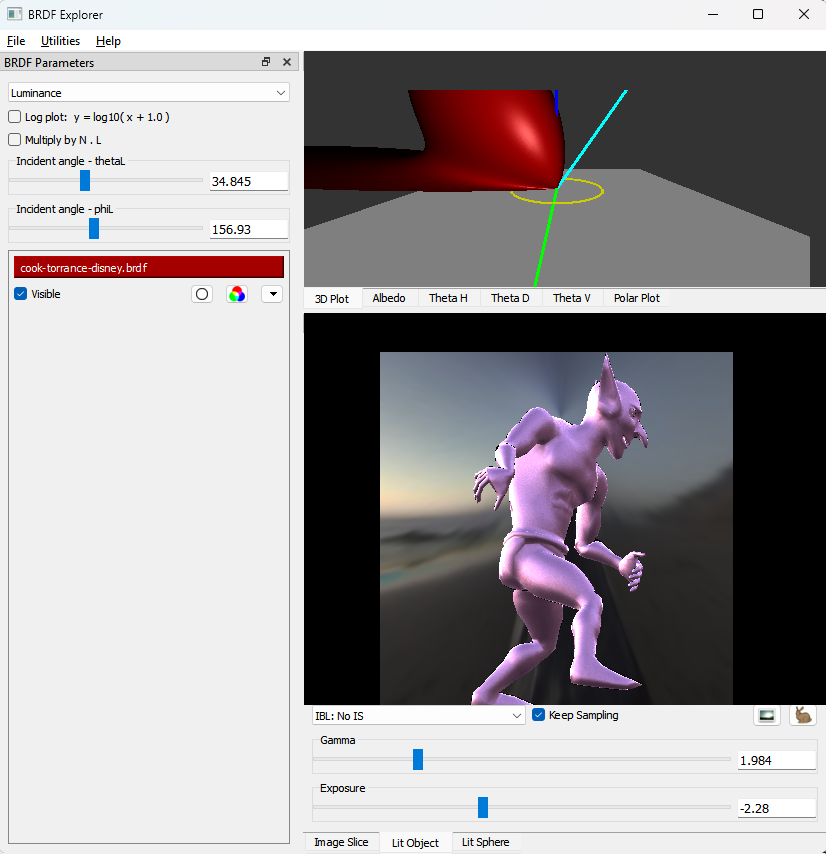
\includegraphics[scale=0.65]{./Imagens/disney-brdf-tool-original.png}
        \end{center}
  \legend{ \small Fonte: autor.}
\end{figure}


\begin{figure}[h]
        \caption{\label{fig-disney-code} \small O código GLSL com sintaxe extra para definir parâmetros.}
        \begin{center}
            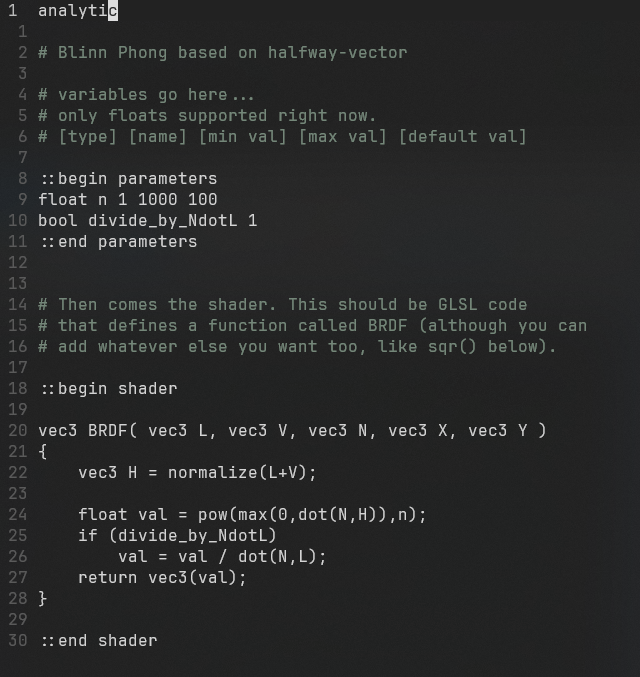
\includegraphics[scale=0.7]{./Imagens/disney-brdf-code.png}
        \end{center}
\end{figure}





% \chapter{Desenvolvimento}

\chapter{Desenvolvimento}

Este capítulo detalha o desenvolvimento do compilador escrito na linguagem Odin, que torna possível a transformação de equações em documentos \LaTeX{} em código GLSL. Cada etapa do processo é encapsulada em um pacote distinto, estruturado em diretórios conforme a \autoref{estrutura-de-pacotes}. O \texttt{lexer} corresponde à tokenização da linguagem, responsável por converter o texto em tokens identificáveis. O \texttt{parser} realiza a análise sintática, construindo a estrutura gramatical do documento. O \texttt{walker} contém funções essenciais para visualização da árvore de sintaxe abstrata (AST) e checagem de tipos feita pelo \texttt{checker}, executando a travessia da árvore de forma ordenada para geração de código feita pelo pacote \texttt{emitter}. A arquitetura completa do compilador pode ser vista na \autoref{fig-estrutura-geral-compilador}.

\begin{figure}[!ht]
  \caption{\label{fig-estrutura-geral-compilador} \small Estrutura de geral da arquitetura do compilador.}
  \begin{center}
    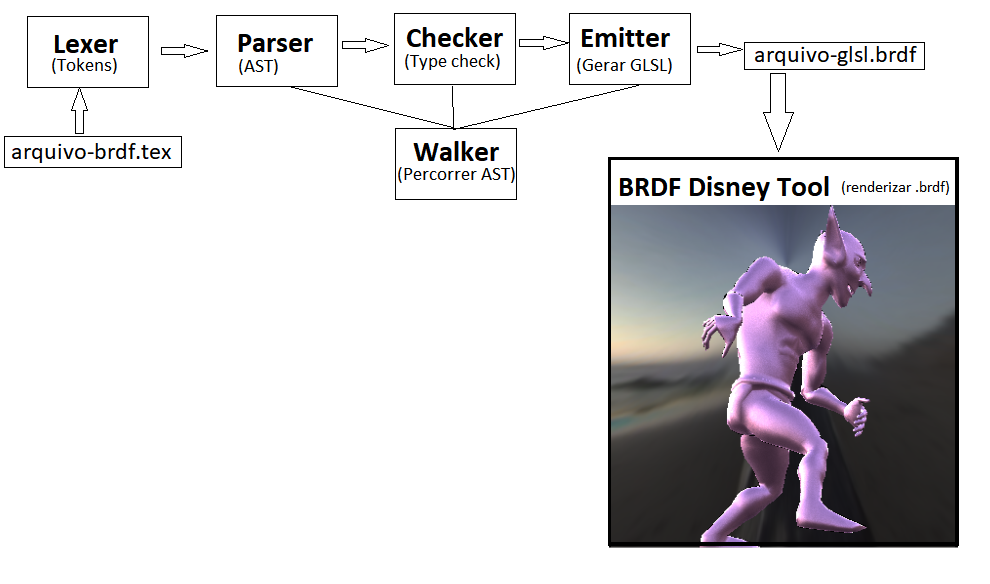
\includegraphics[scale=0.62]{./Imagens/estutura-geral-do-projeto.png}
  \end{center}
\end{figure}


\begin{figure}[!ht]
  \caption{\label{estrutura-de-pacotes} \small Estrutura de pacotes do compilador.}
  \begin{center}
    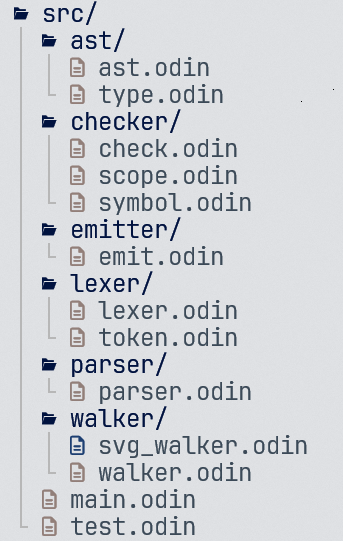
\includegraphics[scale=0.5]{./Imagens/package-structure.png}
  \end{center}
\end{figure}

No módulo \texttt{lexer}, explicado na \autoref{section-lexer}, foi implementado uma análise léxica manual inspirado em máquina de estados para tokenização do documento \LaTeX{}. Este processo converte a entrada textual em uma sequência de tokens, preparando o as estruturas de dados para as próximas etapas de processamento.


Na \autoref{section-parser}, é discutido sobre o pacote \texttt{parser}, que utiliza gramática livre de contexto e a técnica de \textit
{Pratt Parsing} para construir a árvore de sintaxe abstrata (AST). Essa abordagem possibilita uma representação hierárquica precisa das expressões matemáticas de BRDFs, capturando as nuances sintáticas e estruturais do documento original. A especificação da linguagem, apresentada nas \autoref{grammar-ast-pt1} e \autoref{grammar-ast-pt2}, é definida na seção de análise sintática, juntamente com a precedência dos operadores prefixos e infixos.

O componente \texttt{walker}, discutido na \autoref{section-walker}, desempenha funções essenciais para a navegação e análise da AST. Suas funcionalidades incluem tanto a visualização da estrutura gerada quanto a preparação para verificações subsequentes por meio do pacote \texttt{checker}. O papel principal do \texttt{walker} é realizar a travessia dessa árvore de forma genérica, oferecendo suporte para decidir se a travessia deve continuar ou se é necessário retornar de um nó antes de alcançar os nós-folha. Além disso, o componente permite a identificação da profundidade atual da travessia e abstrai a forma de percorrer nós de maneira uniforme, independentemente do tipo do nó.

No módulo de \texttt{checker} (\autoref{section-checker}), foi implementado as  inferências de tipos e validações semânticas. Este componente garante a consistência das expressões matemáticas antes da geração de código com o auxilio da tabela de simbolos, \autoref{subsection-symbols-scopes}, eliminando potenciais erros de modelagem. A saída dessa etapa deve está apta a emitir código GLSL e na ordem correta dos simbolos.

Por fim, o \texttt{emitter} faz uso da AST validada, tabela de símbolos e escopos para gerar código GLSL, transformando expressões matemáticas de BRDFs contidas na AST em um \textit{shader} com toda implementação necessária para ser carregada na ferramenta de visualização Disney Explorer. Os resultados detalhados e experimentos de aplicação do compilador em BRDFs usadas na literatura podem ser consultados no \autoref{chapter.resultados}, onde demonstramos a eficácia da ferramenta na tradução de diversos modelos de BRDFs. Os experimentos também serviram de guia para verificação da corretude da gramática durante seu desenvolvimento.




% \section{Analise Léxica}

\section{Análise Léxica (\texttt{lexer})} \label{section-lexer}


Nesta etapa, é realizado o processo de tokenização de um subconjunto dos símbolos possíveis no ambiente de equação do \LaTeX{}, conforme comentado na \autoref{especificacao-linguagem}. A entrada desse processo são caracteres do arquivo fonte, enquanto a saída é uma sequência lógica desses caracteres, organizada em \textit{tokens}. O código responsável por essa funcionalidade  está contido no pacote \texttt{lexer}.

O processo de análise léxica realiza uma varredura completa no arquivo de entrada, caractere por caractere, para identificar e extrair os \textit{tokens}. Antes de iniciar essa extração, verificamos se o trecho analisado pertence a um ambiente de equação. Essa verificação é feita ao identificar a \textit{string} \verb|\begin{equation}|, que marca o início da extração de \textit{tokens}. Da mesma forma, a delimitação do ambiente se encerra com a \textit{string} \verb|\end{equation}|. Isso permite que o sistema ignore partes do arquivo que não pertencem ao ambiente de equação, como textos explicativos ou outros elementos presentes no mesmo arquivo \texttt{.tex}. Dessa forma, garantimos que a tokenização seja restrita às secções relevantes do código.

    
% Para fins de documentação e maior clareza, definimos uma lista estruturada de expressões regulares que descreve a geração dos \textit{tokens}, apresentada na \autoref{grammar-tokens}\footnote{Vale observar que a "gramática dos \textit{tokens}" não possui atributos típicos de gramáticas livres de contexto, como recursão, símbolo inicial ou lados direitos compostos por não-terminais. Assim, pode ser mais adequado considerá-la como uma lista estruturada de expressões regulares.}.
%
% O alfabeto dessa gramática é composto pelos caracteres do arquivo fonte. Apesar de ser chamada de gramática, ela se assemelha mais a um conjunto de expressões regulares que descrevem padrões utilizados para identificar os \textit{tokens}. A escolha do termo "gramática" reflete a intenção de estabelecer uma a sintaxe de descrição da gramatica que será usada na gramática da análise sintática, a qual faz uso de uma gramática livre de contexto (GLC) para construção da árvore de sintaxe abstrata. Internamente, a geração dos \textit{tokens} é implementada como a simulação de uma máquina de estados finitos, que segue os padrões definidos por essas expressões regulares.

    % Para fins de documentação e maior clareza, definimos uma gramática que descreve a geração dos \textit{tokens}, apresentada na \autoref{grammar-tokens}\footnote{essa gramatica está mais para uma lista}. O alfabeto dessa gramática é composto pelos caracteres do arquivo fonte. Apesar de documentar com uma gramática, a geração dos \textit{tokens} é implementada internamente de maneira semelhante à simulação de uma máquina de estados.

Na lista de expressões regulares (\autoref{grammar-tokens}), definimos os tipos de \textit{tokens}, onde o lado esquerdo do símbolo ``$=$'' corresponde ao tipo de \textit{token}, e o lado direito descreve sua expressão regular. Palavras em letras maiúsculas representam categorias de caracteres, como \texttt{DIGIT}, que denota qualquer dígito de 0 a 9, e \texttt{LETTER}, que cobre letras de \texttt{`a'} a \texttt{`z'}. Já palavras entre aspas simples correspondem a sequências literais de caracteres.

Além disso, utilizamos os seguintes símbolos na notação: ``$*$'' indica zero ou mais ocorrências do caractere especificado; ``$|$'' representa alternativas para a geração do mesmo tipo de \textit{token}; e ``$;$'' marca o fim da definição do tipo de \textit{token}.

%%%%%%%%%%%%%

O pacote inteiro de tokenização pode ser acessado por meio de uma única função, descrita no \autoref{function-lex}, escrita na linguagem \texttt{Odin}. Essa função, chamada \texttt{lex}, aceita uma lista de caracteres como entrada e retorna uma lista de estruturas do tipo \texttt{Token} (detalhado no \autoref{lexer-structs}). A estrutura \texttt{Token} possui três campos principais:

\begin{itemize}
    \item \texttt{kind}: identifica o tipo de \textit{token}, mapeando-o para uma dos tipos definidos no \autoref{grammar-tokens}.
    \item \texttt{text}: contém a \textit{string} correspondente ao \textit{token} gerado.
    \item \texttt{position}: uma instância do tipo \texttt{Position}, que registra a posição exata do \textit{token} no arquivo de origem.
\end{itemize}


\begin{codigo}[H]
        \caption{\small Função principal do Lexer. }
        \label{function-lex}
\begin{lstlisting}[language = c]
  
    lex :: proc(input: []u8) -> []Token
\end{lstlisting}
\end{codigo}



Durante a iteração sobre o \texttt{input}, o processo de tokenização mantém algumas variáveis de controle para monitorar o estado do fluxo de caracteres. Quebras de linha são contadas ao encontrar sequências como \verb|"\n"| ou \verb|"\n\r"|. É mantida a coluna atual que rastreia a posição horizontal do caractere em uma linha. O cursor é o índice que aponta para o caractere atualmente em processamento. Essas informações são usadas para preencher o campo \texttt{position} de cada \textit{token}. A estrutura \texttt{Position}, detalhada no \autoref{lexer-structs}, é essencial para garantir a precisão na geração de relatórios e rastreamento de erros.

\subsection{Reporte de Erros} \label{subsection-erros}

O sistema informação de erros, implementado nesta etapa, é utilizado por todos os pacotes do projeto. Essa funcionalidade assegura que erros sejam associados a posições específicas no arquivo de entrada, facilitando a depuração e correção. A assinatura da função de tratamento de erros, bem como suas possíveis variações, está documentada no \autoref{cod-function-errors}.

\begin{codigo}[H]
    \caption{\small Função de erro exposto pelo pacote \texttt{lexer}. }
        \label{cod-function-errors}
\begin{lstlisting}[language=C++]
error_from_pos :: proc(pos: Position, msg: string, args: ..any)
error_from_token :: proc(token: Token, msg: string, args: ..any);
\end{lstlisting}
\end{codigo}


Dada uma posição ou um \texttt{token}, é exibida uma mensagem (\texttt{msg}) diretamente no terminal, formatada para destacar visualmente o erro em vermelho. A formatação utiliza as informações do \texttt{token}, como o nome do arquivo, a linha, a coluna e o comprimento do \texttt{token} problemático, permitindo sublinhar precisamente onde o erro ocorreu. Isso proporciona maior clareza às mensagens de erro, como exemplificado no caso de erro semântico devido ao uso de identificadores não definidos (\autoref{error-undefined-symbol}).

Optou-se por apresentar nesta seção uma visão geral de alguns erros possíveis para demonstrar como o compilador os reporta visualmente, independentemente de serem léxicos, sintáticos ou semânticos. Essa abordagem evita sobrecarregar as seções de análise sintática e semântica com descrições ou imagens excessivas. Nas análises seguintes, os tipos de erro serão discutidos em suas etapas correspondentes. A seguir, são apresentados exemplos de erros possíveis:

\begin{enumerate}
   \item \textbf{Erros léxicos}: uso de palavras reservadas (\autoref{error-reserved-word}).
   
   \item \textbf{Erros sintáticos}: problemas de estrutura, como balanceamento incorreto de parênteses (\autoref{error-balanceamento}) e \textit{tokens} que não formam uma expressão matemática válida (\autoref{error-cant-make-expression}).
   
   \item \textbf{Erros semânticos}: envolvendo tipos incompatíveis (\autoref{error-incompatible-types}), símbolos não definidos (\autoref{error-undefined-symbol}) e redefinição de símbolos (\autoref{error-redefinition}).
\end{enumerate}


% Outros exemplos de erros seguem o mesmo padrão de exibição e incluem: tipos incompatíveis (\autoref{error-incompatible-types}), símbolos não definidos (\autoref{error-undefined-symbol}), balanceamento de parênteses (\autoref{error-balanceamento}), uso de palavras reservadas (\autoref{error-reserved-word}) .

\begin{figure}[H]
    \caption{\label{error-undefined-symbol} \small Erro ao tentar símbolo não definido.}
    \begin{center}
        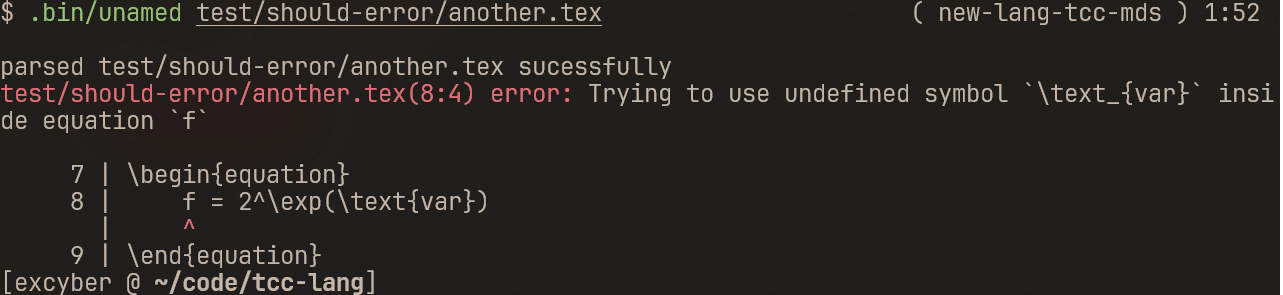
\includegraphics[scale=0.5]{./Imagens/error-undefined-symbol.png}
    \end{center}
\end{figure}

\begin{figure}[H]
    \caption{\label{error-incompatible-types} \small Erro de tipos incompatíveis.}
    \begin{center}
        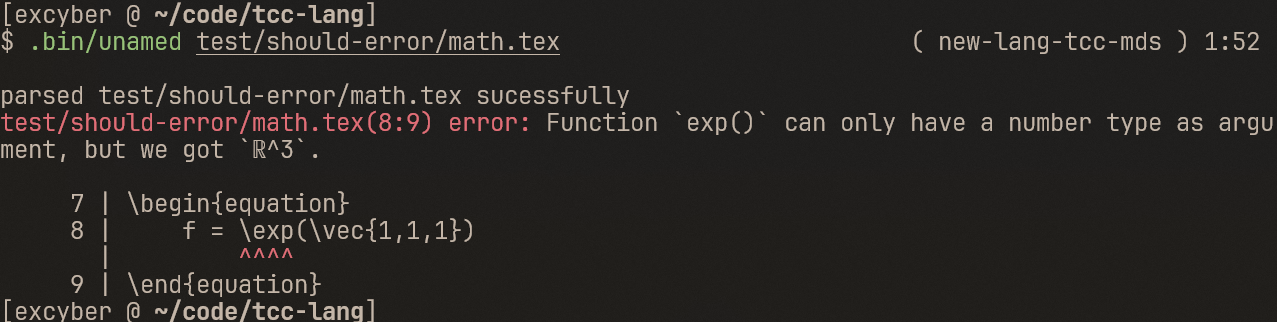
\includegraphics[scale=0.5]{./Imagens/error-incompatible-types.png}
    \end{center}
\end{figure}


\begin{figure}[H]
    \caption{\label{error-balanceamento} \small Erro de balanceamento de parênteses.}
    \begin{center}
        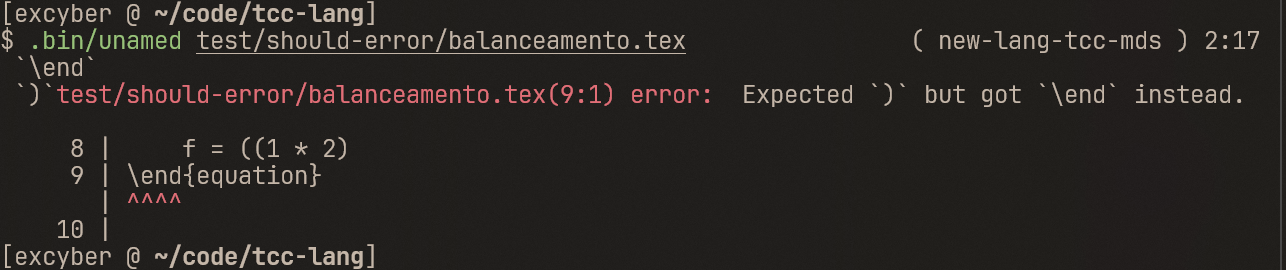
\includegraphics[scale=0.5]{./Imagens/error-balanceamento.png}
    \end{center}
\end{figure}

\begin{figure}[H]
    \caption{\label{error-reserved-word} \small Erro de uso incorreto de palavras reservadas.}
    \begin{center}
        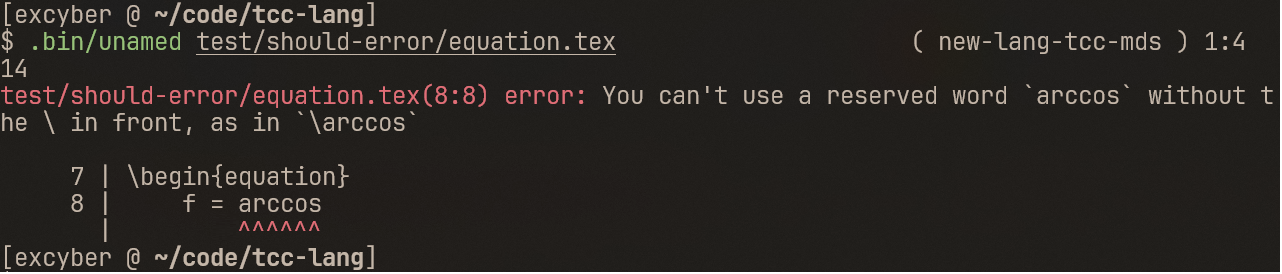
\includegraphics[scale=0.5]{./Imagens/error-reserved-word.png}
    \end{center}
\end{figure}


\begin{figure}[H]
    \caption{\label{error-cant-make-expression} \small Erro de \textit{token} incapaz de produzir expressão.}
    \begin{center}
        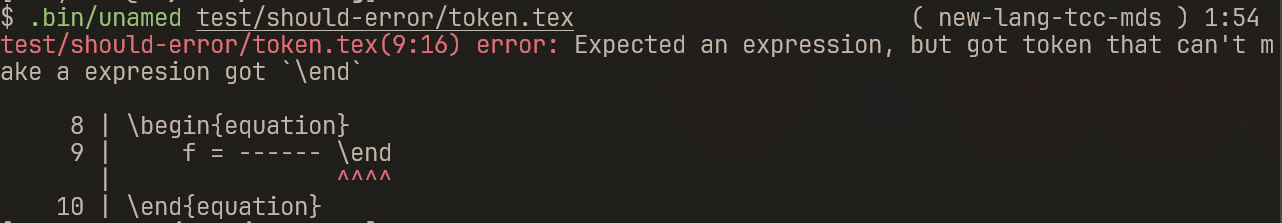
\includegraphics[scale=0.5]{./Imagens/error-cant-make-expression.png}
    \end{center}
\end{figure}

\begin{figure}[H]
    \caption{\label{error-redefinition} \small Erro de redefinição de símbolo.}
    \begin{center}
        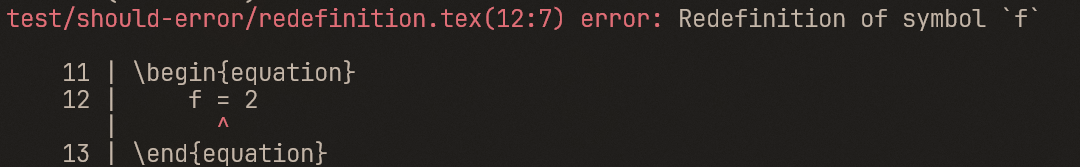
\includegraphics[scale=0.5]{./Imagens/error-redefinition.png}
    \end{center}
\end{figure}



\subsection{Classificação e Extração de Tokens}

Tokens simples, como aqueles compostos por um ou dois caracteres, são extraídos lendo-se o número correspondente de caracteres do \texttt{input}. Após a leitura, o \texttt{token} é construído e o laço continua para o próximo. Quando um caractere \texttt{\%} é encontrado, os caracteres subsequentes são ignorados até a próxima quebra de linha. Isso adiciona suporte a comentários no estilo \LaTeX{}.

Tokens mais complexos, como números, identificadores ou \textit{tokens} especiais, são extraídos com base em suas características. Números podem opcionalmente conter um ponto decimal, como em $1.0$. Já identificadores consistem em uma ou mais letras, opcionalmente prefixadas pelo símbolo \verb|\|.

A lista de expressões regulares de \textit{tokens} fornecida é intrinsecamente ambígua. Por exemplo, uma sequência como \verb|\frac| pode ser interpretada como um identificador comum ou como \verb"token_frac". Para resolver essa ambiguidade, criamos um dicionário que mapeia identificadores específicos para \textit{tokens} especiais (\autoref{map-special-identifiers}). Assim, se um identificador começar com o caractere \verb|\|, ele será verificado no dicionário e classificado como um \textit{token} especial, se apropriado.


\label{lexer-subexpression}
Identificadores não permitem números nem mesmo o caractere de sublinhado (\verb|_|). Isso ocorre porque, no analisador sintático, um nó do tipo identificador é modelado como um tipo recursivo, permitindo que identificadores sejam aninhados ao conter outros nós. Dessa forma, não é necessário permitir sublinhados diretamente no nível de token, o que possibilita a escrita de identificadores mais complexos, como \verb|\pi{n_1}| (renderizado em \LaTeX{} como $\pi_{n_1}$). Nesse caso, \verb|\pi| seria o primeiro \textit{token} do nó identificador, e sua subexpressão seria \verb|n_1| (renderizado como $n_1$), que, por sua vez, é o identificador \verb|n| com a subexpressão \verb|1|.


Adicionalmente, permitimos o uso da palavra-chave \verb|\text|, como em \verb|\text{id}|, para descrever identificadores. Essa palavra-chave é utilizada para incluir texto dentro do ambiente de equações em \LaTeX{}, que pode oferecer uma visualização mais clara de funções longas. Por exemplo, em vez de renderizar `\( normalize(x) \)', pode-se usar \verb|\text{normalize}(x)|, que será renderizado como `\( \text{normalize}(x) \)', tornando a expressão mais legível. Outro caso útil pode ser o \textit{token} `\( len \)', que pode ser visualmente confundido com a multiplicação entre \(l\), \(e\) e \(n\); usando \verb|\text{len}|, fica mais claro que `\(\text{len}\)' é um único \textit{token}, e não como uma multiplicação entre 3 outros \textit{tokens}. A extração do \textit{token} \verb|\text| segue um processo semelhante ao do suporte para \verb|\vec{id}|.

A enumeração que representa os tipos de \textit{tokens} pode ser consultada no \autoref{enum-token-kind}. Cada entrada dessa enumeração corresponde diretamente aos tipos de \textit{tokens} gerados pela lista de expressões regulares apresentada no \autoref{grammar-tokens}. Para facilitar a leitura, incluímos o símbolo correspondente à direita de cada entrada, indicado em comentários.

Com a etapa de tokenização concluída, é possível avançar para a análise sintática, onde é explorada a forma como os \textit{tokens} gerados são organizados em estruturas hierárquicas que formam a árvore sintática.

\begin{codigo}[H]
        \caption{\small Estruturas do Lexer. }
        \label{lexer-structs}
\begin{lstlisting}[language=C++]

Token :: struct {
    kind: Token_Kind,
    val: union{i64,f64},
    text: string,
    pos:  Position,
}

Position :: struct {
    file:   string,
    offset: i64,   // starting at 0, buffer offeset in file
    line:   i64,   // starting at 1, starting
    column: i64,   // starting at 1
    length: int    // how much chars foward
}
    
  \end{lstlisting}
\end{codigo}




\begin{codigo}[H]
    \caption{\small Gramática ilustrativa para \texttt{tokens}. }
        \label{grammar-tokens}
  \begin{lstlisting}[numbers=none, frame=none, language=haskell]

    token_number     = DIGIT DIGIT* '.' DIGIT DIGIT* | DIGIT DIGIT*;
    token_identifier = '\' LETTER LETTER* | LETTER LETTER*;
    token_cmpgreater = '>';
    token_cmpless    = '<';
    token_cmpequal   = '==';
    token_equal      = '=';
    token_mul        = '*' | '\cdot';
    token_cross      = '\times';
    token_div        = '/';
    token_plus       = '+';
    token_minus      = '-';
    token_caret      = '^';
    token_semicolon  = ';';
    token_comma      = ',';
    token_colon      = ':';
    token_question   = '?';
    token_bang       = '!';
    token_openparen  = '(';
    token_closeparen = ')';
    token_opencurly  = '{';
    token_closecurly = '}';
    token_tilde      = '~';
    token_underline  = '_'; --- Used for subexpresions
    token_arrow      = '->';
    token_begin      = '\begin';
    token_end        = '\end';
    token_frac       = '\frac';
    token_vec        = '\vec';
    token_omega      = '\omega';
    token_theta      = '\theta';
    token_phi        = '\phi';
    token_rho        = '\rho';
    token_alpha      = '\alpha';
    token_beta       = '\beta';
    token_sigma      = '\sigma';
    token_pi         = '\pi';
    token_epsilon    = '\epsilon';
    token_max        = '\max';
    token_min        = '\min';
    token_exp        = '\exp';
    token_tan        = '\tan';
    token_sin        = '\sin';
    token_cos        = '\cos';
    token_arctan     = '\arctan';
    token_arcsin     = '\arcsin';
    token_arccos     = '\arccos';
    token_sqrt       = '\sqrt';
    token_text       = '\text';
    token_eof        = EOF;
    
  \end{lstlisting}
\end{codigo}



\begin{codigo}[H]
\caption{\small Enumeração dos tipos de \texttt{tokens}. }
    \label{enum-token-kind}
\begin{lstlisting}[language = C++]
  Token_Kind :: enum {
    EOF           = 0,
    Number,
    Identifier,

    Equal,        // =
    Mul,          // * ou \cdot
    Cross,        // X
    Div,          // /
    Plus,         // +
    Minus,        // -
    Caret,        // ^
    Comma,        // ,
    Colon,        // :
    Question,     // ?
    Bang,         // !
    OpenParen,    // (
    CloseParen,   // )
    OpenCurly,    // {
    CloseCurly,   // }
    Tilde,        // ~
    Underline,    // _
    Arrow,        // ->

    Begin = 256,  // \begin
    End,          // \end

    Frac,         // \frac
    Vec,          // \vec

    Omega,        // \omega
    Theta,        // \theta
    Phi,          // \phi
    Rho,          // \rho
    Pi,           // \pi
    Epsilon,      // \epsilon
    Alpha,        // \alpha
    Beta,         // \beta
    Sigma,        // \sigma

    Max,          // \max
    Min,          // \min
    Exp,          // \exp
    Tan,          // \tan
    ArcTan,       // \arctan
    Sin,          // \sin
    ArcSin,       // \arcsin
    Cos,          // \cos
    ArcCos,       // \arccos
    Sqrt,         // \sqrt

    Text,         // \text
    Invalid
}

\end{lstlisting}
\end{codigo}

\begin{codigo}[H]
        \caption{\small Mapa de identificadores especiais. }
        \label{map-special-identifiers}
  \begin{lstlisting}[language=C++]

SPECIAL_WORDS := map[string]Token{
    "text"  = Token{text = "\\text",     kind =.Text},

    // Special
    "frac"   = Token{text = "\\frac",    kind =.Frac},
    "vec"    = Token{text = "\\vec",     kind =.Vec},
    "cdot"   = Token{text = "\\cdot",    kind =.Mul},
    "begin"  = Token{text = "\\begin",   kind =.Begin},
    "end"    = Token{text = "\\end",     kind =.End},
    "rho"    = Token{text = "\\rho",     kind =.Rho},
    "sqrt"   = Token{text = "\\sqrt",    kind =.Sqrt},
    "omega"  = Token{text = "\\omega",   kind =.Omega},

    // Cross product
    "times"  = Token{text = "\\times",   kind =.Cross},

    "max"    = Token{text = "\\max",     kind =.Max},
    "min"    = Token{text = "\\min",     kind =.Min},
    "exp"    = Token{text = "\\exp",     kind =.Exp},

    "cos"    = Token{text = "\\cos",     kind =.Cos},
    "sin"    = Token{text = "\\sin",     kind =.Sin},
    "tan"    = Token{text = "\\tan",     kind =.Tan},

    "arccos" = Token{text = "\\arccos",  kind =.ArcCos},
    "arcsin" = Token{text = "\\arcsin",  kind =.ArcSin},
    "arctan" = Token{text = "\\arctan",  kind =.ArcTan},

    "theta"  = Token{text = "\\theta",   kind =.Theta},
    "phi"    = Token{text = "\\phi",     kind =.Phi},

    "alpha"   = Token{text = "\\alpha",  kind =.Alpha},
    "beta"    = Token{text = "\\beta",   kind =.Beta},
    "sigma"   = Token{text = "\\sigma",  kind =.Sigma},
    "pi"      = Token{text = "\\pi",     kind =.Pi},
    "epsilon" = Token{text = "\\epsilon",kind =.Epsilon},
}

    
  \end{lstlisting}
\end{codigo}


% \section{Analise Sintática}

\section{Análise Sintática, (\texttt{parser})} \label{section-parser}

O \textit{parser} para a linguagem subconjunto do ambiente \verb|equation| do \LaTeX{} foi desenvolvido utilizando o método de Pratt \textit{Parsing} na linguagem Odin. Neste contexto, denominamos esse subconjunto como \texttt{EquationLang}, que abrange todas as partes essenciais para a definição de BRDFs descritas em \autoref{especificacao-linguagem}, além de sua gramática documentada.

A implementação deste \textit{parser} adota o método de descida recursiva, no qual cada regra de produção da gramática possui uma função de análise correspondente. Este método foi escolhido por priorizar a clareza e simplicidade do código, complementados por comentários detalhados para facilitar a compreensão. A entrada do \textit{parser} consiste nos \textit{tokens} gerados na etapa de análise léxica.


\subsection{Parser}

Diferentemente dos \textit{parsers} tradicionais de descida recursiva, que frequentemente utilizam múltiplas chamadas de função aninhadas para tratar diferentes níveis de precedência, o \textit{parser} aqui implementado organiza as funções de análise de forma hierárquica, com base na precedência dos operadores. Essa abordagem é detalhada no \autoref{alg-pratt-parsing}, que descreve a lógica central para o \textit{parsing} de expressões.

%%%%%%%%%%%%%%%%
Pratt Parsing simplifica a análise sintática de expressões ao tratar precedência e associatividade dinamicamente, sem inflar a gramática. Na abordagem tradicional, precedências são fixadas por meio de várias regras de produção, desmontrado no \autoref{cod-regras-tradicionais}.

\begin{codigo}[htb]
    \caption{\small Regras tradicionais de precendecia por gramática. }
    \label{cod-regras-tradicionais}
\begin{lstlisting}[language=haskell, numbers=none, inputencoding=utf8]
    Expr               = LogicalOrExpr;
    LogicalOrExpr      = LogicalOrExpr      '||' LogicalAndExpr    | LogicalAndExpr;

    LogicalAndExpr     = LogicalAndExpr     '&&' EqualityExpr      | EqualityExpr;

    EqualityExpr       = EqualityExpr       '==' RelationalExpr    | RelationalExpr;   ---  Igualdade


    RelationalExpr     = RelationalExpr     '<' AdditiveExpr       | AdditiveExpr;     ---  Comparação

    AdditiveExpr       = AdditiveExpr       '+' MultiplicativeExpr | MultiplicativeExpr;

    MultiplicativeExpr = MultiplicativeExpr '*' PrimaryExpr        | PrimaryExpr;

    PrimaryExpr        = '(' Expr ')' | NUMBER | Identifier;  --- Expressões primárias

\end{lstlisting}
\end{codigo}


Isso torna a gramática mais longa, necessitando de mais regras que derivam outras regras antes de chegar a um símbolo do alfabeto da gramática. Na descrição recursiva, regras são o mesmo que funções, o que significa que os métodos recursivos tradicionais com muitos níveis de precedência fazem mais chamadas recursivas em código, gerando mais lentidão e complexidade na implementação da descrição recursiva a ser mantida. No Pratt Parsing, uma única regra é suficiente:
\verb`Expr = Expr ( '||' | '&&' | '==' | '<' | '+' | '*' ) Expr;`.

A precedência é definida em uma tabela (\autoref{tab-token-precedence}), e o \textit{parser} consulta essa tabela dinamicamente para decidir a ordem de avaliação com base no operador encontrado. Isso reduz a complexidade, facilita alterações e melhora a eficiência do \textit{parser}, resultando em um código mais simples, eficiente e flexível para incluir novos operadores.

Foi usado a notação similiar à original de Pratt \cite{pratt}, as funções \verb"parse_null_denotations" e \texttt{parse\_left\_denotations} desempenham papéis equivalentes às funções \texttt{token.prefixo} e \texttt{token.infixo}, respectivamente, como demonstrado no \autoref{alg1}. Além disso, a abordagem de descida recursiva (top-down) permite que cada regra de produção definida na gramática (\autoref{grammar-ast-pt1}) seja diretamente mapeada para um procedimento em código. Isso pode ser observado, por exemplo, na função de análise do nó \texttt{Start} da AST (\autoref{cod-parsing-start}), que reflete diretamente as regras de produção \texttt{start}, \texttt{decl}, e \texttt{decl\_equation\_begin\_end\_block} especificadas na gramática demonstrada no \autoref{grammar-ast-pt1}.

Do ponto de vista da interface oferecida pelo pacote \texttt{parser}, todo o processo de análise sintática é abstraído em uma única chamada de função (\autoref{cod-func-and-structs}). A função principal, \texttt{parse}, trabalha em conjunto com a estrutura \texttt{Parser} para realizar a análise.

\begin{codigo}[H]
  \caption{\small Parsing de expressão em código Odin.}
        \label{alg-pratt-parsing}
  \begin{lstlisting}[language=C]


parse_expr :: proc(prec_prev: i64) -> ^Expr {
    /* expressions that takes nothing (null) as left operand */
    left := parse_null_denotations()
    /*
    . if current token is left associative or current token has higher precedence
    . than previous precedence then stay in the loop, effectively creating a left leaning
    . sub-tree, else, we recurse to create a right leaning sub-tree.
    */
    for precedence(peek()) > prec_prev + associativity(peek())  {
        /* expressions that needs a left operand such as postfix, mixfix, and infix operator */
        left = parse_left_denotations(left)
    }
    return left
}


  \end{lstlisting}
\end{codigo}

\begin{codigo}[htb]
        \caption{\small Estruturas e Funções do Parser. }
        \label{cod-func-and-structs}
  \begin{lstlisting}[language = C]
Parser :: struct {
    tokens:      []Token,
    cursor:      i64,
    error_count: int,
}

parse :: proc(using p: ^Parser) -> ^ast.Start {
    return parse_start(p)
}
  \end{lstlisting}
\end{codigo}

\begin{codigo}[htb]
    \caption{\small \textit{Parsing} do nó \texttt{Start}. }
        \label{cod-parsing-start}
  \begin{lstlisting}[language=C++]
parse_start :: proc(using p: ^Parser) -> ^ast.Start {
    node := ast.new(ast.Start)
    decls := [dynamic]^ast.Decl{}

    for peek(p).kind != .EOF {
        decl := parse_equation_begin_end_block(p)
        append(&decls, decl)
    }
    node.eof = next(p, Token_Kind.EOF)
    node.decls = decls[:]
    return node
}
    
  \end{lstlisting}
\end{codigo}



\subsection{Gramática}

Para formalizar a gramática da linguagem de entrada (\texttt{EquationLang}), estabelecemos regras detalhadas nos \autoref{grammar-ast-pt1} e \autoref{grammar-ast-pt2}. O \autoref{code-gramatica} apresenta um exemplo de código-fonte válido nesta linguagem, cuja renderização correspondente em \LaTeX{} é ilustrada em \autoref{code-gramatica-rendered}.

\label{code-gramatica-rendered} \begin{subequations}
\begin{equation}
    \rho_{d} = \vec{0.3,0.3,0.3}
\end{equation}
\begin{equation}
    \rho_{s} = \vec{0.0,0.2,1.0}*20
\end{equation}
\begin{equation}
f = \frac{\rho_{d}}{\pi} + \frac{\rho_{s}}{8*\pi} *
\frac{({\vec{n}}\cdot{\vec{h}})}
{({\vec{\omega_{o}}}\cdot{\vec{h}}) *
\max(({\vec{n}}\cdot{\vec{\omega_{i}}}),
({\vec{n}}\cdot{\vec{\omega_{o}}}))}
\end{equation}
\end{subequations}


\begin{codigo}[htb]
        \caption{\small Exemplo código escrito na linguagem \texttt{EquationLang}. }
        \label{code-gramatica}
\begin{lstlisting}[language=tex, frame=none]
\begin{equation}
    \rho_{d} = \vec{0.3,0.3,0.3}
\end{equation}

\begin{equation}
    \rho_{s} = \vec{0.0,0.2,1.0}*20
\end{equation}

\begin{equation}
f = \frac{\rho_{d}}{\pi} + \frac{\rho_{s}}{8*\pi} *
\frac{({\vec{n}}\cdot{\vec{h}})}
{({\vec{\omega_{o}}}\cdot{\vec{h}}) *
\max(({\vec{n}}\cdot{\vec{\omega_{i}}}),
({\vec{n}}\cdot{\vec{\omega_{o}}}))}
\end{equation}

\end{lstlisting}
\end{codigo}

\begin{codigo}[H]
        \caption{\small Gramática para \texttt{EquantionLang} parte 1.}
        \label{grammar-ast-pt1}
\begin{lstlisting}[language=haskell, numbers=none, inputencoding=utf8]
    start  = decl* token_eof;

    decl = decl_equation_begin_end_block;

    decl_equation_begin_end_block =
        token_begin token_opencurly 'equation' token_closecurly
        decl_equation
        token_end token_opencurly 'equation' token_closecurly;

    decl_equation = field;

    field = expr token_equal expr;

    expr = expr_identifier
        | expr_number
        | expr_vector_literal
        | expr_grouped
        | expr_prefix
        | expr_infix
        | expr_postfix
        --- Ressalto que `function_call` e `function_definition` tem a mesma construção.
        --- Apenas diferenciamos pela posição que aparecer, se à esquerda ou à direta de '=' da regra `field`.
        --- por exemplo `a = f(1)`, `f(1)` é uma chamada de função
        --- Já `f(x) = 1` é uma definição de função
        | expr_function_call
        | expr_function_definition
        | token_opencurly expr token_closecurly
    ;

    expr_identifier =
        --- Ex: `\text{id}`
        token_text token_opencurly expr_identifier token_closecurly
        --- Ex: `\vec{id}`
        token_vec token_opencurly expr_identifier token_closecurly
        --- Ex: `id_n`
        | expr_identifier token_underline expr_identifier
        --- Ex: `id_2`
        | expr_identifier token_underline token_number
        --- Ex: `id_{n+1}`
        | expr_identifier token_underline token_opencurly expr token_closecurly
        --- Token especiais como \phi ou \alpha
        | token_identifier
        | token_omega
        | token_theta   | token_phi
        | token_rho     | token_alpha
        | token_beta    | token_sigma
        | token_pi      | token_epsilon
        | token_max     | token_min
    ;

\end{lstlisting}
\end{codigo}

\begin{codigo}[H]
        \caption{\small Gramática para \texttt{EquantionLang} parte 2.}
        \label{grammar-ast-pt2}
\begin{lstlisting}[language=haskell, numbers=none, inputencoding=utf8]
    expr_number = token_number;

    expr_vector_literal = token_vec
        --- Ex: `\vec{1, 1, 1}`
        token_opencurly
        (expr_number token_comma)* expr_number
        token_closecurly
    ;

    expr_grouped = token_openparen expr token_closeparen;

    expr_prefix =
        (token_sqrt | token_exp | token_tan| token_cos | token_sin | token_arctan | token_arccos | token_arcsin | token_minus | token_plus) expr
    ;

    expr_infix = token_frac
        token_opencurly expr token_closecurly
        token_opencurly expr token_closecurly
        | expr token_plus     expr
        | expr token_minus    expr
        | expr token_mul      expr
        | expr token_cross    expr
        | expr token_cmpequal expr
        | expr token_div      expr
        | expr token_caret    expr
    ;

    expr_postfix = expr token_bang;

    expr_function_call = expr token_openparen
        (expr token_comma)* expr
        token_closeparen
    ;

    --- Mesmo que expr_function_call, em etapas posteriores é decidido qual tipo realmente é.
    expr_function_definition = expr token_openparen
        (expr token_comma)* expr
        token_closeparen
    ;
\end{lstlisting}
\end{codigo}

Na definição da gramática (\autoref{grammar-ast-pt1}), adotamos a notação sintática previamente estabelecida na \autoref{section-lexer}, com o adicional que sequências de três hífens ("\verb"---"") representam comentários para o leitor, sem impactar a definição gramatical.

A gramática definida nesta seção abrange regras para expressões, atribuições, agrupamento, literais numéricos e vetores, chamadas de funções, definições de funções e diversos operadores, como \texttt{expr\_prefix} e \texttt{expr\_infix}. O objetivo é fornecer uma linguagem capaz de expressar a sintaxe necessária para definições de BRDFs em \LaTeX{}. 

A tabela de operadores (\autoref{tab-token-precedence}) usada no Pratt Parsing é representada pela função \texttt{precedence\_from\_token}, que mapeia um token para um valor inteiro que representa sua precedência: quanto maior o valor, maior a precedência do operador. É importante observar que alguns tokens podem ser usados tanto como prefixos quanto como infixos, dependendo do contexto. Por exemplo, o token \texttt{(} pode ser um prefixo em uma expressão de agrupamento, como em \textbf{(}$2*3$\textbf{)}, mas também pode ser infixo em uma chamada de função, como em $f$\textbf{(}$x$\textbf{)}. O mesmo comportamento ocorre com o token \texttt{-}, que pode atuar como operador prefixo de negação ou infixo para subtração.


\begin{table}[h!]
\centering
\begin{tabular}{|l|c|c|}
\hline
\textbf{Tipo de Token} & \textbf{Prefixo} & \textbf{Precedência}\\ \hline
\texttt{+}            & Sim              & 25                   \\ \hline
\texttt{-}            & Sim              & 25                   \\ \hline
\texttt{(}            & Sim              & 100                  \\ \hline
\texttt{:}            & Sim              & 100                  \\ \hline
\texttt{*}            & Sim              & 100                  \\ \hline
% \texttt{\textasciitilde} & Sim              & 200               \\ \hline
\texttt{!}            & Sim              & 300                  \\ \hline
\texttt{(}            & Não              & 500                  \\ \hline
\texttt{>}            & Não              & 5                    \\ \hline
\texttt{<}            & Não              & 5                    \\ \hline
\texttt{+}            & Não              & 10                   \\ \hline
\texttt{-}            & Não              & 10                   \\ \hline
$\times$              & Não              & 20                   \\ \hline
\texttt{*}            & Não              & 20                   \\ \hline
\texttt{/}            & Não              & 20                   \\ \hline
\texttt{\textasciicircum} & Não           & 30                  \\ \hline
\texttt{!}            & Não              & 400                  \\ \hline
\end{tabular}
\caption{Tabela de Precedência dos Tokens}
\label{tab-token-precedence}
\end{table}


\subsubsection{Estrutura da Árvore de Sintaxe}
Nesta seção, apresentamos os tipos de nós que compõem a árvore de sintaxe abstrata (AST), utilizada no compilador da linguagem \texttt{EquationLang}. A estrutura da AST é formada por diversos tipos de nós que capturam os diferentes elementos da sintaxe da linguagem. Diferente da gramática definida no \autoref{lst-gramatica}, os nós aqui são representados em nível de código. Vale ressaltar que o nó \texttt{Expr}, o mais genérico, possui um campo adicional \texttt{ty\_inferred} do tipo \texttt{Type}. Esse campo será preenchido durante a etapa de análise semântica e utilizado na geração de código. A seguir, listamos a representação semântica de cada nó, detalhando os campos que compõem cada um deles.

@@Fix this
\begin{itemize}
\item \textbf{Node}: Estrutura base para todos os nós da AST.
      \textbf{Campos:}
      \texttt{kind} (\texttt{typeid}), guarda um número que indica qual o tipo do nó.

\item \textbf{Expr}: Representa expressões de forma geral.
      \textbf{Campos:}
      \texttt{expr\_derived} e \texttt{ty\_inferred} (\texttt{Type})

\item \textbf{Decl}: Representa genericamente declarações.

\item \textbf{Start}: O nó raiz da AST.
      \textbf{Campos:}
      \texttt{decls} lista de \texttt{Decl}, \texttt{eof} (\texttt{Token}).

\item \textbf{Decl\_Equation}: representa uma equação.
      \textbf{Campos:}
      \texttt{field} referencia à uma instancia do nó (\texttt{Field}).

\item \textbf{Field}: Representa uma atribuição qualquer, usando o simbolo '='.
      \textbf{Campos:}
      \texttt{name} (\texttt{\^Expr}), \texttt{equals} (\texttt{Token}), \texttt{value} (\texttt{\^Expr}).

\item \textbf{Expr\_Identifier}: Representa identificadores.
      \textbf{Campos:}
      \texttt{identifier} (\texttt{Token}), \texttt{is\_vector} (\texttt{bool}),
      \texttt{sub\_expression} (\texttt{\^Expr}), \texttt{var} (\texttt{Maybe(string)}).

\item \textbf{Expr\_Number}: Representa literais numéricos.
      \textbf{Campos:}
      \texttt{number} (\texttt{Token}).

\item \textbf{Expr\_Vector\_Literal}: Representa vetores literais.
      \textbf{Campos:}
      \texttt{vec} (\texttt{Token}), \texttt{numbers} (\texttt{[]\^Expr\_Number}).

  \item \textbf{Expr\_Grouped}: representa expressões agrupadas, geralmente por \(\), mas é permitido agrupor por \{\}.
      \textbf{Campos:}
      \texttt{open} (\texttt{Token}), \texttt{expr} (\texttt{\^Expr}), \texttt{close} (\texttt{Token}).

  \item \textbf{Expr\_Prefix}: representa expressão com operator prefixo (ex: -3).
      \textbf{Campos:}
      \texttt{op} (\texttt{Token}), \texttt{right} (\texttt{\^Expr}).

  \item \textbf{Expr\_Infix}: representa expressões para operador infixo, isto é entre expressões, (ex: 3+3).
      \textbf{Campos:}
        \texttt{left} (pointeiro de \texttt{Expr}), \texttt{op} (\texttt{Token}), \texttt{right} (pointeiro de \texttt{Expr}).

\item \textbf{Expr\_Function\_Call}: representa chamadas de função.
      \textbf{Campos:}
      \texttt{left} (ponteiro de \texttt{Expr}), \texttt{open} (\texttt{Token}),
      \texttt{exprs} (lista de poteiros de \texttt{Expr}), \texttt{close} (\texttt{Token}).

\item \textbf{Expr\_Function\_Definition}: representa definições de funções.
      \textbf{Campos:}
      \texttt{name} (\texttt{Expr\_Identifier}), \texttt{open} (\texttt{Token}),
      \texttt{parameters} (lista de \texttt{Expr\_Identifier}), \texttt{close} (\texttt{Token}).
\end{itemize}




No \autoref{lexer-subexpression}, é comentado que o \textit{parser} é capaz de lidar com identificadores aninhados, como, por exemplo, \( x_{i_1} \) (\verb"x_{i_1}"). No \autoref{cod-expression-ident-recursive}, apresentamos como esses identificadores são criados recursivamente. O código mostrado faz parte de uma função maior, sendo um recorte de um \texttt{switch}\footnote{\texttt{switch} e \texttt{case} em Odin funcionam da mesma forma que na linguagem de programação \texttt{C}} sobre a enumeração descrita no \autoref{enum-token-kind}. Dentro desse \texttt{switch}, temos um \texttt{case} que reconhece tokens de identificador ou símbolos especiais (\( \omega, \theta, \phi, \rho, \alpha, \beta, \sigma, \pi, \epsilon \)). Ao fazer uma chamada recursiva à função \texttt{parse\_expr}, o \textit{parser} permite a inclusão de subíndices numéricos, subexpresões de identificadores ou até expressões binárias, como \( n+1 \) em \( f_{n+1} \).

Isso confere maior flexibilidade na hora de expressar funções e equações para descrever as BRDFs, sendo muito comum o uso de subíndices numéricos. Na etapa de geração de código, essa capacidade de distinguir identificadores com subíndices é crucial, pois permite tratar semânticamente tokens aparentemente iguais de maneira diferenciada. Por exemplo, embora o primeiro token seja \( f \), \( f_1 \) e \( f_2 \) são semanticamente distintos, permitindo uma distinção precisa entre símbolos com o mesmo nome base, mas com significados diferentes devido aos seus índices.
%%%%%


\begin{codigo}[htb]
    \caption{\small Parte do código de \textit{parsing} de expressão para identificadores. }
        \label{cod-expression-ident-recursive}
  \begin{lstlisting}[language = C]
    case .Identifier,
         .Omega,     // \omega
         .Theta,     // \theta
         .Phi,       // \phi
         .Rho,       // \rho
         .Alpha,     // \alpha
         .Beta,      // \beta
         .Sigma,     // \sigma
         .Pi,        // \pi
         .Epsilon,   // \epsilon
        node := ast.new(ast.Expr_Identifier)
        node.identifier = next(p)
        if peek(p).kind == Token_Kind('_') {
            next(p)
            if peek(p).kind == Token_Kind('{') {
                next(p, '{')
                node.sub_expression = parse_expr(p, prec)
                next(p, '}')
            } else {
                //
                // If we're not using `identifier_{ }` then, we only allow simple number or identifier
                //
                sub_node := ast.new(ast.Expr_Identifier)
                if peek(p).kind == .Number {
                    // We only allow number as sub expressions
                    sub_node.identifier = next_expects_kind(p, .Number)
                } else {
                    sub_node.identifier = next_expects_kind(p, .Identifier, ..SPECIAL_IDENTIFIERS[1:])
                }
                node.sub_expression = sub_node
            }
        }
    
  \end{lstlisting}
\end{codigo}


O \autoref{cod-expression-ident-recursive}, já apresentado, serve como exemplo para outras expressões recursivas, como expressões infixas (operações binárias). Para identificar o token atual, utilizamos a função \texttt{peek()}, que permite visualizar um ou dois tokens à frente e, com isso, decidir qual nó da AST (Árvore de Sintaxe Abstrata) deve ser construído. Após identificar o token, calculamos a variável \texttt{prec}, que indica a precedência do token atual. Com base nessa precedência, fazemos uma ou mais chamadas recursivas à função \texttt{parse\_expr} para processar os campos que requerem expressões aninhadas.

Uma vez que todos os campos necessários estejam preenchidos, a expressão completa é retornada. Esse processo é repetido até que a subárvore de expressões de uma dada equação esteja completamente construída. A análise sintática é concluída quando todas as equações forem adicionadas à AST. Essa estrutura hierárquica das expressões é então anotada com tipos e validada pelo pacote \texttt{checker}, conforme discutido na \autoref{secion-checker}.

No entanto, antes que a validação ocorra, é necessário implementar métodos para realizar a travessia dessa estrutura. O processo de travessia da AST é discutido na seção \autoref{secion-walker}, onde são apresentadas as técnicas para percorrer a árvore e acessar os dados nela contidos, facilitando a análise semântica e a geração de código subsequente.




\section{Implementação do Padrão de Visitante (\texttt{walker})}

Desenvolvemos o pacote \textit{walker} para auxiliar em 3 tarefas chaves: validação de precedencia da AST gerada pelo \textit{parser}; visualização da AST gráficamente; geração de código. O padrão visitante foi empregado para percorrer e operar em uma AST. Uma estrututa e uma função implementam esse padrão e agem em cima da AST. procedimentos implementam esse padrão e manipulam a AST: \texttt{Visitor} e \texttt{walk}, respectivamente.


O padrão visitor implementado na função \texttt{walk} representa um mecanismo genérico e recursivo para travessia da AST, permitindo a aplicação de transformações ou análises personalizadas em cada nó da árvore.

A estrutura \texttt{Visitor} (\autoref{cod-visitor-struct}) encapsula uma função de visita polimórfica que pode ser chamada para cada tipo de nó, possibilitando um processamento flexível e extensível, onde o visitante pode modificar seu próprio estado durante a travessia, decidir continuar ou interromper o caminhamento, e realizar operações arbitrárias como transformação, análise semântica, geração de código ou depuração.

A função, no \autoref{cod-visitor-walk} implementa uma travessia profunda (\textit{depth-first}) recursiva, que automaticamente percorre todos os nós da AST, incluindo declarações, expressões, statements e estruturas aninhadas, invocando a função de visita antes e depois da exploração de cada subárvore. Isso é utils para criação de visitors personalizados para diferentes propósitos como checagem de tipos, parentização de expressões, geração de gráficos para arvóre.


\begin{codigo}[htb]
    \caption{\small Estrutura polimórfica \texttt{Visitor}}
        \label{cod-visitor-struct}
\begin{lstlisting}[language = C]

// Estrutura polimórfica, aceita um tipo qualquer, chamado de DataType, como estrada para criar um tipo concreto.
Visitor :: struct (DataType: typeid) {
    visit: proc(visitor: ^Visitor(DataType), node: ^ast.Node) -> ^Visitor(DataType),
    data:  DataType,
}
\end{lstlisting}
\end{codigo}

\begin{codigo}[tb]
\caption{\small Estrutura \texttt{Visitor} e função de percurso \texttt{walk}. }
        \label{cod-visitor-walk}
\begin{lstlisting}[language = C]
// Por brevidade vamos omitir varios casos do `switch` que seguem a mesma lógica
walk :: proc(v: ^Visitor($T), node: ^ast.Node) {
    if v == nil || node == nil {
        return
    }
    v := v->visit(node)
    if v == nil {
        return
    }
    using ast
    switch n in &node.derived {
        case ^Start:
            for d in n.decls {
                walk(v, d)
            }

        case ^Decl_Equation:
            walk(v, n.field)

        case ^Field:
            walk(v, n.name)
            walk(v, n.value)

        case ^Expr_Number:     // Caso base

        case ^Expr_Vector_Literal:
            for number in n.numbers {
                walk(v, number)
            }
        case ^Expr_Identifier:
                walk(v, n.sub_expression)

        // ...
        // casos OMITIDOS aqui Também
        // ...
        case ^Expr_Infix:
            walk(v, n.left)
            walk(v, n.right)

        case ^Expr_Grouped:
            walk(v, n.expr)

        case ^Expr_Function_Call:
            walk(v, n.left)
            for e in n.exprs {
                walk(v,  e)
            }
        case:
            assert(false, "Unhandled token on walk_print ")
    }
    v = v->visit(nil)
}

  \end{lstlisting}
\end{codigo}


\subsection{Validação de Precedencia}
Utilizamos o pacote \texttt{walker} para validão precendencia de operadores na AST gerada pelo \texttt{parser}. A função de parentização implementa inserção automática de parênteses que captura a precedência original das operações na AST, garantindo que a representação textual preserve a ordem de avaliação das expressões matemáticas. Através de uma travessia disponivel pelo pacote usado, o algoritmo cria uma cadeia de caraceters com parênteses adicionais em expressões com prefixo, expressões binárias, chamada de funções. Isso é feita todas as os tipos de expressões. 
Essa reprodução explicita da hierarquia de operações permite verificar automaticamente se a construção da AST durante o parsing manteve corretamente as regras de precedência.

Cada teste de precendecia consiste em um texto original e um testo com parenteses esperaros, como demonstrado na listagem \autoref{cod-test-paren}. Tentamos testar os casos mais complexos de expressões matemáticas, operações como exponenciação, que é associativo pela direitoa, combinado com operadores associativo pela esquerda  com diferentes precedencias

À medida que o compialdor foi sendo desenvolvido esses testes se mostraram uteis em previnir quebra do de casos anteriores, pois ao dar suporte a nova funcionalidade, é possivel quebrar funcionalidade já estabelicidade anterioromente.
,\begin{itemize}
  \item \textbf{walker\_interp}: interpreta a AST, calculando o valor numérico das expressões.
  \item \textbf{walker\_paren}:   \item \textbf{walker\_print}: imprime os nós da AST e seus atributos, facilitando a depuração e compreensão da estrutura da AST.

\end{itemize}
\begin{codigo}[htb]
    \caption{\small Teste de precendencia usando por parentização. }
        \label{cod-test-paren}
  \begin{lstlisting}[language = C]
    test_paren(
        `a = 1+2`, // Entrada
        `a=(1+2)`  // Saída Esperada
    )

    test_paren(
        `a = \exp 1 + 2^3`, // Entrada
        `a=(\exp(1)+(2^3))` // Saída Esperada
    )

    // ...
    // Outros Testes
    // ...

    test_paren(
        `a = a(1*2 ^ 4 +  \sqrt 4^8 , 2)`, // Entrada
        `a=a(((1*(2^4))+(\sqrt(4)^8)),2)`  // Saída Esperada
    )
  \end{lstlisting}
\end{codigo}



\subsection{Visualização da AST por Imagem}

Para validação visual, foi implementado um função que gera uma imagem no formato ``SVG``, que é um formato textual, da arvore contendo informação circulos, representados nós da AST, jutamente com textos subinscritos informados metadados sobre os nós, como o tipo de operador, o tipo de nó, a string do indetificador  no caso de ser @etc.

Como exemplo, na \autoref{fig-svg} temos a visualização do SVG gerado pela equação \autoref{eq-svg}. Notamos que os nós '+' e '-' próximo da raiz seriam avaliados depois, já os nós mais próximo das folhas deve ser resolvidos primeiros indicando um precedencia maior, como expressões binárias '*' e '^'. Esse SVG também anota o tipo da expressão, (note que "v" é do tipo \mathbb{R}^3), é feito na estapa de checker, veremos mais a frente como isso é feito.
 

@@@
Os nós são heterogeneos, a maneira de acessar um filho de cada nós depende do tipo, pois o campo varia de nome ou posição na es trutura, o pacote walker também permite extrair nós filhos de maneira uniforme para qualquer tipo de nó através de uma função chamada children (\autoref{cod-childre-signature}).(funções como ``children`` que dado um nó abstrato, ele resolve qual o tipo resolvido e cria um array de nós, como extrair os filho). Ela é usada para simplificar o código de geração do SVG ao agir em cima de um nó de maneira uniforme, sem se preocupar com o tipo do nó.

\begin{codigo}[htb]
        \caption{\small Assinatura da função que extrai nós filhos de maniera uniforme para qualquer tipo de nó. }
        \label{cod-childre-signature}
  \begin{lstlisting}[language = C]
    // Aceita um ponteiro de nós abstrato e return uma lista de nós filhos
    children :: proc(node: ^Node) -> (array :[dynamic]^Node);
  \end{lstlisting}
\end{codigo}



% Temos dois tipos de validação dessa precendencia para garantir corretude de implementação de Pratt Parser, uma visual e outra automatica.
% Como mostrado em \autoref{tab-token-precedence} usamos uma tabela para definir a priopridade de operadores,
%
%
% ```
% \begin{equation}
% opertattions ungrouped
%
% \end{equation}
% ```
% Já se agruparmos certas operações, temos e o SVG gerado é diferente mostrando mostrando-se util em auxiliar o desenvolvimento.
%
%
% ```
% \begin{equation}
% grouped
% \end{equation}
% ```
% A maneira automatica é feita utilizando tested que gerandados sobre os casos, cada caso tem um entrada dada e saida esperada. A entrada é uma equação em string, a saída é uma string com a mesma, mas com a ordem de operação explicitamente citada através de parensentese. à Medida que o compialdor foi sendo desenvolvido mais teste foram adicionado para previnir quebra do código a medida que o projeto foi avançando. Alguns exemplos se encontram em @@@ e a informação gerada após aplicar o texto esta em @@@. Adicionamos o parentese através de um outro modulo chamado ``walker``, nele temos acesso à funções como ``children`` que dado um nó abstrato, ele resolve qual o tipo resolvido e cria um array de nós, como extrair os filho de nós heterogeneos precisa ser abstraido, cada estruttura tem campos diferetnes como filho. Outra facilidade que esse pacote desenvolvido é o padrão visitador @@ pegar o padrão visitador que tem função que utiliza generics.
%
%
% ```odin
% SVG_Node :: struct{
%     name: string,
%     children: [dynamic]^SVG_Node,
% };
% ```
% Como mostrado em @@@ usamos uma tabela para definir a priopridade de operadores
% Criamos um tabela que define e atráves de uma função, podemos acessar esses valores
% dado um token temos o reusltado
% Temos dois tipos de validação dessa precendencia para garantir correture de implementação de Pratt Parser, uma visual e outra automatica.
% Para validação visual, foi implementado um função que gera uma imagem no formato ``svg`` da arvore contendo informação circulos, representados nós da AST, jutamente com textos subinscritos informados metadados sobre os nós, como o tipo de operador, o tipo de nó, a string do indetificador  no caso de ser @etc
% Os nós próximo da raiz seriam implementados depois, já os proximos das folhas deve ser resolvikdos pprimeiros indicando um precedencia maior por exemplo
%
% Compilado para gerar a AST em SVG da equação @@, esperamos que '^' ocorra antes '*' que ocorra antes. Ao observar a arvore, notamos que o nó correspondente àoperação '^' ocorre.
%
% ```
% \begin{equation}
% opertattions ungrouped
%
% \end{equation}
% ```
% Já se agruparmos certas operações, temos e o SVG gerado é diferente mostrando mostrando-se util em auxiliar o desenvolvimento.
%
%
% ```
% \begin{equation}
% grouped
% \end{equation}
% ```
% A maneira automatica é feita utilizando tested que gerandados sobre os casos, cada caso tem um entrada dada e saida esperada. A entrada é uma equação em string, a saída é uma string com a mesma, mas com a ordem de operação explicitamente citada através de parensentese. à Medida que o compialdor foi sendo desenvolvido mais teste foram adicionado para previnir quebra do código a medida que o projeto foi avançando. Alguns exemplos se encontram em @@@ e a informação gerada após aplicar o texto esta em @@@. Adicionamos o parentese através de um outro modulo chamado ``walker``, nele temos acesso à funções como ``children`` que dado um nó abstrato, ele resolve qual o tipo resolvido e cria um array de nós, como extrair os filho de nós heterogeneos precisa ser abstraido, cada estruttura tem campos diferetnes como filho. Outra facilidade que esse pacote desenvolvido é o padrão visitador @@ pegar o padrão visitador que tem função que utiliza generics.
%
%
% ```odin
% SVG_Node :: struct{
%     name: string,
%     children: [dynamic]^SVG_Node,
% };
% ```
%
%
% \subsection{Testes}
%
%
% Foi desenvolvida uma série de testes que  abrangem vários aspectos da funcionalidade do \textit{parser}, incluindo geração de árvore de sintaxe, precedência de operadores e interpretação semântica.
%
%
% \subsubsection{Geração de Árvore de Sintaxe}
%
%
% Um aspecto crucial dos testes envolve verificar a correta geração de árvores sintáticas a partir de expressões de entrada. Os testes são projetados para cobrir diferentes cenários, incluindo operações aritméticas simples, expressões complexas com sub-expressões aninhadas e chamadas de funções. São eles:
%
%
% \begin{itemize}
%     \item O manuseio correto de operadores unários e binários, garantindo a precedência e associatividade adequadas.
%     \item A representação precisa de chamadas de função e seus argumentos dentro da árvore de sintaxe.
%     \item O agrupamento adequado de expressões dentro de parênteses para confirmar regras de precedência.
% \end{itemize}


\section{Análise Semântica (\texttt{checker})} \label{section-checker}
O processo de validação semântica no compilador é crucial para garantir a corretude das equações, a consistência de tipos em operações e a resolução adequada de símbolos. Ele é estruturado em dois mecanismos principais: validação de definições de funções e validação de declarações. Esses mecanismos trabalham de forma integrada para garantir que a estrutura do programa esteja em conformidade com as regras semânticas da \texttt{EquationLang}.

Nesta seção, abordamos essas regras e discutimos como são validadas expressões envolvendo vetores, redefinições de equações e possíveis erros nas definições de BRDFs que inviabilizem a geração de código. A conclusão bem-sucedida dessa etapa de inferência e validação indica que o programa está apto a prosseguir para a fase de geração de código GLSL, conduzida pelo pacote \texttt{emitter}.


\subsection{Funções do Pacote \texttt{checker}}

O pacote \texttt{checker} é responsável por realizar diversas tarefas fundamentais para a validação semântica do compilador. Essas tarefas são descritas detalhadamente a seguir:

\begin{enumerate}
    \item \textbf{Inferência e Anotação de Tipos}:
    Cada expressão na AST possui um campo \verb"ty_inferred" que deve ser preenchido durante essa etapa. Para determinar esses tipos, é necessário realizar a inferência de tipos. Essa tarefa é detalhada na \autoref{subsection-type-inference}. Os tipos possíveis incluem números (\verb"float"), vetores (\verb"vector") e funções.
        O tipo de uma função é representada por um domínio (tipos dos argumentos de entrada) e um contradomínio (tipo do valor de retorno). Exemplos incluem:
        \begin{itemize}
            \item Uma função $f(a, b) = a \cdot b \cdot \vec{1,1,1}$, que recebe dois valores reais e retorna um vetor tridimensional, possui a assinatura:
            \[
            f : \mathbb{R} \times \mathbb{R} \to \mathbb{R}^3.
            \]
            \item O produto vetorial, que combina dois vetores tridimensionais, possui a assinatura:
            \[
            \times : \mathbb{R}^3 \times \mathbb{R}^3 \to \mathbb{R}^3.
            \]
        \end{itemize}
        Essas assinaturas são coletadas durante o processo de inferência para garantir a consistência em expressões de chamada de funções.

    \item \textbf{Compatibilidade de Tipos}:
    O \texttt{checker} também verifica a compatibilidade entre tipos em diferentes contextos do programa. Essa validação assegura que:
    \begin{itemize}
        \item Não sejam realizadas operações não definidas por \texttt{EquationLang}, como a divisão entre dois vetores.
        \item Não sejam aplicados operadores em tipos incompatíveis, como elevar um número a um vetor ($2^{\vec{n}}$).
        \item Os argumentos de uma função devem pertencer ao domínio esperado pela função. Por exemplo, se a função $\texttt{normalize}(\vec{u})$ retorna um vetor tridimensional ($\mathbb{R}^3$), utilizá-lo como argumento para a função seno, que espera um número escalar ($\mathbb{R}$), seria inválido. Assim, $\sin(\texttt{normalize}(\vec{u}))$ não é permitido.
        \item O tipo do valor de retorno de uma função deve ser compatível com o contexto em que é utilizado.
    \end{itemize}

    \item \textbf{Validação de Definições de Símbolos}:
        Outro papel fundamental do \texttt{checker} é garantir que todos os identificadores, abstraídos em símbolos na \autoref{subsection-symbols-scopes}, utilizados no programa, estejam devidamente definidos antes de serem usados. Essa etapa inclui:
    \begin{itemize}
        \item Identificar declarações ausentes.
        \item Identificar dependência circular.
        \item Certificar-se de que funções obrigatórias, como a BRDF $f$, estejam presentes.
    \end{itemize}
\end{enumerate}

Essas validações são realizadas utilizando as funções do pacote \textit{walker}, e os erros encontrados são reportados usando as funções de erro introduzidas na \autoref{section-lexer}.

% \subsection{Uso do Padrão Visitor}
% @@@ Prefisamos manter essa subseção se já vamos detalhar mais pra frente?@@
%
% Para realizar a validação semântica, o pacote \texttt{walker} é reutilizado, permitindo a travessia modular da AST. Essa abordagem facilita a aplicação recursiva de inferência de tipos, provida pelo, mesmo em expressões aninhadas.
%
% Validações ocorrem nessa traversia e basedo no tipo do nó, a inferencia é feita, discutido na \autoref{subsection-inferencia-tipos} uma operação binária de multiplicação:
% \begin{itemize}
%     \item Se ambos os operandos forem números reais, o resultado também será um número real.
%     \item Se um dos operandos for um vetor tridimensional, o resultado dependerá do outro operando (por exemplo, um escalar ou outro vetor).
% \end{itemize}
%
% Como a esquerda ou a direita de uma operação binária podem ser expressões aninhadas (outras operações binárias, chamadas de funções, etc.), o padrão visitor permite aplicar a inferência de tipos recursivamente. Esse processo garante que o tipo de cada subexpressão seja determinado de forma consistente e confiável.
%

\subsection{Tipos, Símbolos e Escopos} \label{subsection-symbols-scopes}

Cada expressão na AST possui um tipo associado, modelado como uma união de estruturas na linguagem Odin. Essa união permite representar as seguintes categorias semânticas: tipos primitivos fundamentais, como números e vetores; assinaturas de funções, que capturam o domínio e o contradomínio. Por exemplo, o produto vetorial possui a assinatura $\mathbb{R}^3 \times \mathbb{R}^3 \to \mathbb{R}^3$. Já o vetor normal ($\vec{n}$), possui tipo primitivo de número ($\mathbb{R}$). A modelagem clara de tipos e o conceito de escopos e símbolos é essencial para validar expressões em diferentes contextos, verificar compatibilidade de operações e garantir a consistência semântica do programa.


\subsubsection{Tipos}

No \autoref{cod-types-structs}, a representação dos tipos segue uma modelagem hierárquica, onde o \textbf{tipo base} (\texttt{Type}) contém metadados comuns, como a referência ao nó na árvore sintática e o identificador do tipo concreto. Os \textbf{tipos derivados}, que são subdivididos em categorias específicas, incluem: \textit{tipo básico} (\texttt{Type\_Basic}), que representa um tipo primitiva como um número; \textit{tipo vetorial} (\texttt{Type\_Vector}), que é caracterizado pela sua dimensionalidade e pelo tipo de elemento que o compõe; e \textit{tipo função} (\texttt{Type\_Function}), que define os parâmetros e os resultados da função.

\begin{codigo}[H]
    \caption{\small Estruturas que representam os tipos de expressões da AST.}
    \label{cod-types-structs}
\begin{lstlisting}[language=C, numbers=none, frame=none, inputencoding=latin1]

Type :: struct {
    node:    ^Node,
    size:    i64,
    derived: Any_Type, // Ou Type_Vector, ou Type_Basic, ou Type_Function.
    id:      typeid,
}

Type_Vector :: struct {
    using _:      Type,
    element_type: ^Type,
    dimensions:   int,
}


Type_Basic :: struct {
    using _: Type,
    basic_kind : Basic_Kind,
};


Type_Function :: struct {
    using _: Type,
    params, results :[]^Type,
};

\end{lstlisting}
\end{codigo}


\subsubsection{Símbolos}

Os símbolos representam entidades nomeadas em \texttt{EquationLang}. A estrutura \texttt{Symbol}, apresentada no \autoref{cod-symbol}, encapsula as informações semânticas necessárias sobre os identificadores para validação da AST e geração de código. Essas informações incluem: \begin{itemize} \item \textbf{Escopo}: o escopo em que o símbolo foi definido. \item \textbf{Nó do identificador}: referência ao nó correspondente na AST para uso futuro. \item \textbf{Definição de função (opcional)}: nó da definição de função, quando aplicável. \item \textbf{Estado de resolução}: indica se o símbolo já foi resolvido. \item \textbf{Tipo associado}: o tipo inferido ou declarado do símbolo. \end{itemize}

O gerenciamento de símbolos é essencial para garantir que o estado de cada símbolo seja mantido durante a resolução, como discutido na \autoref{subsection-sym-resolution}. Os possíveis estados são listados a seguir:
\begin{enumerate}
    \item \textbf{Não Resolvido:} Estado inicial
    \item \textbf{Em Progresso:} Resolução em andamento
    \item \textbf{Resolvido:} Completamente processado
\end{enumerate}

\begin{codigo}[H]
    \caption{\small Estrutura do Símbolo.}
    \label{cod-symbol}
\begin{lstlisting}[language=C, numbers=none, frame=none, inputencoding=latin1]
// An Symbol is a named entity in the language
Symbol :: struct  {
    scope:      ^Scope,

    identifier: ^ast.Expr_Identifier, // Can be nullptr
    fn_defn:    ^ast.Expr_Function_Definition, // if the Symbol is a function

    state:      Symbol_State,
    flags:      bit_set[Symbol_Flag; u64],
    type:       ^Type,
    value:      Maybe(Value)
};

\end{lstlisting}
\end{codigo}


\subsection{Escopo e Tabela de Símbolos} \label{section-escope-table}


Nesta etapa, foi criada uma tabela de símbolos para análise semântica e geração de código GLSL. A implementação da tabela de símbolos fornecida aqui é baseada em uma estrutura de escopo hierárquico, onde cada escopo mantém um mapeamento entre os nomes dos símbolos e seus atributos correspondentes. No \autoref{struct-symbol}, a estrutura \texttt{Scope} representa um mapeamento de nomes para objetos de símbolo dentro de um \textbf{único escopo}, e a estrutura \texttt{Scope\_Table} mantém uma \textbf{pilha de escopos}, permitindo aninhamento.

\begin{codigo}[H]
\caption{\small Código da estrutura de símbolos escrito em Odin.}
\label{struct-symbol}
\begin{lstlisting}[language=C]
Scope_Table :: [dynamic]^Scope

Scope :: struct {
/*
 . `node` Is a parent node that created that scope
 . Ex: a block, a function block, a struct or namespace
 . If null, then the scope is the global
*/
    parent:   ^Scope,
    children:   [dynamic]^Scope,
    elements: map[string]^Symbol,
    ordered_keys: []string, // bit of a HACK, yeah
};

\end{lstlisting}
\end{codigo}

A tabela de símbolos fornece funções para gerenciar escopos, incluindo:
\begin{itemize}
    \item \texttt{scope\_enter}: entrar em um novo escopo, anexando-o à pilha de escopos.
    \item \texttt{scope\_exit}: sai do escopo atual, removendo-o da pilha de escopos e o retornando.
    \item \texttt{scope\_get}: recupera um símbolo da tabela de símbolos pelo seu identificador.
    \item \texttt{scope\_add}: adiciona um novo símbolo ao escopo atual.
\end{itemize}

Essa tabela de símbolos armazena todas as informações necessárias para a fase de geração do \textit{shader} GLSL.


\subsection{Resolução de Símbolos} \label{subsection-sym-resolution}
A resolução de símbolos é uma etapa fundamental no \texttt{checker}, garantindo que cada símbolo seja corretamente definido e tipado antes de seu uso. Esse processo é especialmente relevante em situações onde a ordem de definição não segue um fluxo linear, como no exemplo da \autoref{eq-preref}).

Um escopo global é criado contendo todos os símbolos definidos, e a validação verifica se cada identificador está presente no escopo atual. Caso contrário, é gerado um erro apropriado. É nesta etapa que verificamos se a função $f$, a BRDF por convenção, existe no escopo global. Identificadores embutidos, definidos pelas convenções deste trabalho como $\omega_i$ e $\theta_d$, são adicionados automaticamente à tabela de símbolos juntamente com seus tipos. A lista completa de embutidos está disponível em \autoref{cod-builtins}. Símbolos de parâmetros são resolvidos no escopo da função correspondente.


%%%%


Nesse caso da \autoref{eq-preref}, \texttt{b} é atribuído a \texttt{a} antes que \texttt{a} seja definido. O \texttt{checker} deve resolver essa dependência, analisando \texttt{a} antes de \texttt{b} para inferir corretamente o tipo de \texttt{b}. Isso é possível por conta da construção de um grafo de dependências entre símbolos (apresentado no \autoref{cod-symbol-graph}). A partir de uma ordenação topológica desse grafo, o sistema determina uma ordem de avaliação válida, além de identificar dependências circulares que possam impedir a compilação.

\begin{subequations} \label{eq-preref}
\begin{equation}
    b = a
\end{equation}
\begin{equation}
    a = \vec{n}
\end{equation}
\begin{equation}
    f = b
\end{equation}
\end{subequations}


Essa ordenação permite usar símbolos antes de suas equações serem declaradas, desde que definidos em alguma equação posterior. A resolução mantém em memória uma lista com a ordem correta de avaliação das declarações, o que é essencial para a geração de código GLSL, onde referências a variáveis antes de suas definições são proibidas.

Para implementar essas funcionalidades, o \texttt{checker} realiza múltiplas passadas na AST: duas são para resolução de símbolos e a última é para validação das equações, na seguinte ordem:

\begin{enumerate}
    \item \textbf{Coleta de Símbolos}:
    \begin{itemize}
        \item Coletar todos identificadores nas declarações
        \item Registrar símbolos nos escopos apropriados
        \item Inicializar estruturas de rastreamento de dependências.     \end{itemize}

    \item \textbf{Análise de Dependências}:
    \begin{itemize}
        \item Construir o grafo de dependências. Estruturas podem ser vistas no \autoref{cod-symbol-graph}, um simples grafo que associa um símbolo a outros símbolos dos quais depende
        \item Validar referências de símbolos, incluindo detectar uso de símbolos que nunca foram definidos
        \item Estabelecer a ordem de avaliação por meio de ordenação topológica
        \item Verificação do ponto de entrada
    \end{itemize}

    \item \textbf{Validação Final}:
    \begin{itemize}
        \item Inferência e verificação de tipos
        \item Validação de expressões
        \item Validação de definição de funções com uso de escopo
    \end{itemize}
\end{enumerate}

\begin{codigo}[H]
\caption{\small Estrutura de grafo de dependências.}
    \label{cod-symbol-graph}
\begin{lstlisting}[language=C, frame=none, inputencoding=utf8]
Symbol_Dependency :: struct {
    dependencies: [dynamic]^Symbol,
}
Symbol_Graph :: map[^Symbol]Symbol_Dependency
\end{lstlisting}
\end{codigo}

% Cosegue lidar com escopo, parametros de funções e simbolos embutidos, aqueles padrões dinifidos na tabela de convenções de simbolos matematiccos \autoref{@va trabahlhar vagabundo@}. Para isso exist multiplas passadas. A primeira coleta todos os simbolos. A segunda, analisa as dependencias e estabelece a ordem de avaliação. Por ultimo, o \texttt{checker} toma contra do restante das inferencias de tipos e outras validações

\begin{codigo}[H]
    \caption{\small Entrada para o compilador que gera dependência circular.}
    \label{cod-grafo-simbol-deps}
\begin{lstlisting}[language=C, numbers=none, frame=none, inputencoding=latin1]
\begin{equation}
    a = f
\end{equation}

\begin{equation}
    f = a
\end{equation}

\end{lstlisting}
\end{codigo}

\begin{figure}[H]
    \caption{\label{label} \small Erro reportado sobre dependencia circular.}
    \begin{center}
        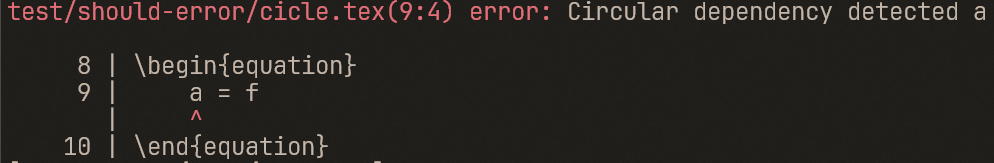
\includegraphics[scale=0.5]{./Imagens/error-circular-deps.png}
    \end{center}
\end{figure}


\subsection{Inferência de Tipos} \label{subsection-type-inference}


A função \verb`infer_type` determina o tipo de uma expressão (\verb`expr`) na AST durante a análise semântica, aplicando regras baseadas em operações matemáticas, como multiplicação entre número real e vetor, produto vetorial entre vetores e assinaturas de funções. 

Projetada para processar todas as expressões de \texttt{EquationLang} — como identificadores, operadores, chamadas de função e literais —, a função verifica inicialmente se o tipo já foi inferido (\verb"expr.ty_inferred") para evitar processamento redundante. Caso contrário, realiza a inferência com base em um \verb"switch" que é capaz de avaliar todos tipos de expressões. Um trecho relevante desse processo está no \autoref{cod-type-inference}, que ilustra a discriminação e validação dos tipos.

Para \textbf{identificadores} (\verb"Expr_Identifier"), verifica se o identificador corresponde a um vetor especial, como $\omega_i$ ou $\vec{n}$. Nesse caso, o tipo é inferido como $\mathbb{R}^3$ (vetor tridimensional). Identificadores específicos, como \verb"\pi" ou \verb"\epsilon", são atribuídos ao tipo numérico real ($\mathbb{R}$). Para outros identificadores, a função consulta o escopo atual para determinar o tipo, usando as estruturas detalhado na \autoref{section-escope-table}.

\begin{codigo}[htb]
    \caption{\small Parte do switch da inferencia de tipos. }
    \label{cod-type-inference}
\begin{lstlisting}[language=C, frame=none, inputencoding=utf8]
infer_type :: proc(expr: ^ast.Expr, allow_invalid := false, default : ^ast.Type = ast.ty_invalid ) -> ^Type {
    /// Código omitido por brevidade  ///
    #partial switch e in expr.derived {
    case ^Expr_Identifier:
        // Alway set by the parser if indentifier starts with `\vec{}`
        if e.is_vector {
            type = new_type_vector(ty_number, 3) // vector 3 of type number (real)
        } else if e.identifier.kind == .Pi || e.identifier.kind == .Epsilon {
            type = ty_number
        } else {
            key := key_from_identifier(e)
            sym, ok := scope_get(key)
            if ok {
                if sym.type != nil {
                    type = sym.type
                }
            }
            /// Código omitido por brevidade  ///
        }

    case ^Expr_Prefix:
        right_type := infer_type(e.right, allow_invalid, default)
        /// Código omitido, mas aqui fazemos a validação da subexpressão direita e atribuimos o tipo correto para Expr_Prefix   ///

    case ^Expr_Infix:
        ty_left  := infer_type(e.left, allow_invalid, default)
        ty_right := infer_type(e.right, allow_invalid, default)
        /// Código omitido
        //  Inferimos tipo da expressão esquerda e direto dessa operação binária
        //  Depois validamos compatibilidade considerando a operação sendo usada nessas duas expressões

    /// Outros casos ...  ///
}
\end{lstlisting}
\end{codigo}


Para \textbf{operações prefixadas} (\verb"Expr_Prefix"), como raiz quadrada (\verb"\sqrt") ou funções trigonométricas (\verb"\sin", \verb"\cos"), a função valida se o operando é numérico e atribui o tipo correspondente à expressão. Nas \textbf{operações binárias} (\verb"Expr_Infix"), a função realiza a inferência dos tipos dos operandos esquerdo e direito. Se os tipos não forem compatíveis, aplica regras específicas. Alguma dessas regras são:

\begin{itemize}
    \item A multiplicação de um número por um vetor ($2*\vec{n}$) ou a divisão de um vetor por um número ($\frac{\vec{u}}{\sqrt{\vec{u} \cdot \vec{u}}}$) resultam no tipo vetor ($\mathbb{R}^3$).
    \item Operações entre dois números resultam em um número.
    \item Operações entre dois vetores resultam em um número ou um vetor a depender se a operação foi um produto vetorial ou produto interno.
\end{itemize}

Outros casos incluem \textbf{literais}, como números (\verb"Expr_Number") e vetores literais \\(\verb"Expr_Vector_Literal"), cujos tipos são atribuídos diretamente como $\mathbb{R}$ (números reais) e $\mathbb{R}^3$ (vetores tridimensionais), respectivamente.



Para chamadas de função (\verb"Expr_Function_Call"), o tipo da expressão é determinado pelo tipo do primeiro valor retornado pela função. A validação dos argumentos é realizada em outra função, detalhada na \autoref{subsubsection-eq-func-defn}. % ; Essa parte já foi dita
% Além disso, a função realiza validações específicas para evitar inconsistências, como garantir que operações entre vetores sejam semanticamente válidas (e.g., divisão entre vetores não é permitida). 

% Em resumo, \verb`infer_type` é uma implementação robusta e flexível de inferência de tipos, essencial para a análise semântica de um compilador. A função assegura que cada expressão receba um tipo coerente com a semântica da linguagem, lidando com uma ampla gama de construções sintáticas e oferecendo suporte extensível para futuras adições à linguagem.

\subsection{Validação de Equações}

As declarações de equações são validadas após a coleta e ordenação descritas na \autoref{subsection-sym-resolution}, portanto assume-se que o lado esquerdo das equações seja um identificador válido ou uma definição de função e que estão na ordem correta de avaliação.

Qualquer violação semântica, como incompatibilidades de tipos ou uso de escalares onde vetores são esperados, é reportada ao usuário, com detalhes sobre o contexto e a localização do erro, conforme descrito em \autoref{subsection-erros}.

A função \verb"check_expr" realiza uma travessia semelhante à inferência de tipos e chama \texttt{infer\_type}. Nela, a análise de expressões que não foram abordadas por \texttt{infer\_type} é realizada para todos os tipos de expressões. Algumas dessas validações estão listadas após este parágrafo, e um trecho dessa travessia pode ser visto no \autoref{eq-function-check-expr}.

\begin{itemize}
    \item \verb`Expr_Function_Call`: Verifica se estamos fazendo a chamada corretamente com um identificador, evitando casos como tentar chamar uma função com um número, por exemplo, $123(x,y)$, o que é incorreto. Também checa se o número de argumentos corresponde ao número de parâmetros esperados.
    \item \verb`Expr_Prefix`: Verifica operadores (\verb`-`, \verb`+`) e funções como \verb`sqrt(x)` e \verb`sin(x)`. Certifica-se de que os tipos sejam compatíveis, gerando erro em caso contrário, como quando um vetor é passado para a função seno.
    \item Literais de Vetor \verb`Expr_Vector_Literal`: Garante que os vetores tenham exatamente 3 dimensões\footnote{Exigir vetores de apenas 3 dimensões pode ser considerado uma limitação semântica imposta pelo compilador}.
\end{itemize}




\begin{codigo}[H]
    \caption{\small Identificadores embutidos pela convenção deste trabalho.}
    \label{cod-builtins}
\begin{lstlisting}[language=C, numbers=none, frame=none, inputencoding=latin1]
BUILTIN_IDENTIFIERS :: []string {
    `\pi`,
    `\epsilon`,
    `\theta{h}`,
    `\vec{n}`,
    `\vec{h}`,
    `\vec{\omega{i}}`,
    `\theta{i}`,
    `\phi{i}`,
    `\vec{\omega{o}}`,
    `\theta{o}`,
    `\phi{o}`,
    `\theta{h}`,
    `\theta{d}`,
}
\end{lstlisting}
\end{codigo}


\begin{codigo}[H]
    \caption{\small Recorte da função \texttt{check\_expr}. }
    \label{eq-function-check-expr}
\begin{lstlisting}[language=C, basicstyle=\ttfamily\footnotesize, frame=none, inputencoding=utf8]
check_expr :: proc(expr: ^ast.Expr) {
    // Primeiro inferimos o tipo
    infer_type(expr)
    // Código omitido de preambulo
        case ^Expr_Identifier:
            // Check for using undefined indetifiers
            identifier_key := key_from_identifier(e)
            if !is_defined(e, false) {
                error(e.identifier,  "Identifier `%v` is not defined in the current scope.", identifier_key)
            }
        case ^Expr_Function_Call:
            check_expr(e.left)
            fn_ident, fn_ident_ok := e.left.expr_derived.(^ast.Expr_Identifier)
            if !fn_ident_ok {
                error(e.open,  "Tried to call an expression that is not an identifier")
            }
            fn_string := key_from_identifier(fn_ident)
            fn_sym, fn_sym_ok := scope_get(fn_string)
            fn_type, fn_type_ok := e.left.ty_inferred.derived.(^ast.Type_Function)
            if !fn_type_ok {
                error(e.open,  "Tried to call`%v`, which is not a function. Its type is `%v`", fn_string, format_type(e.left.ty_inferred))
            }
            if len(e.exprs) != len(fn_type.params) {
                error(
                    e.open,  "Args number mismatch. `%v` function expects  `%v` arguments but `%v` were given.",
                    fn_string, len(fn_type.params), len(e.exprs)
                )
            }
        // Outros casos omitidos
    }
}

\end{lstlisting}
\end{codigo}



\subsection{Validação de Funções}
A validação semântica de definições e chamadas de funções segue um processo semelhante ao da análise de expressões, mas com o uso da pilha de escopos.
Nas definições de funções, as variáveis no corpo da função são validadas para assegurar que todos os símbolos usados realmente estejam definidos no escopo da função. Já nas chamadas de funções, os argumentos fornecidos são comparados aos parâmetros esperados para validação.

\subsubsection{Definição de Funções} \label{subsubsection-eq-func-defn}

O procedimento \verb"check_function_definition" valida definições de funções, garantindo segurança de tipos e consistência através das seguintes tarefas:

\begin{enumerate}
    \item Inferir os tipos dos parâmetros.
    \item Inferir o tipo de retorno baseado na expressão final.
    \item Construir o tipo completo da função, incluindo parâmetros e retorno.
    \item Garantir que os identificadores usados estejam consistentes com seus tipos declarados.
    \item Validar as expressões no corpo da função.
    \item Criar um novo escopo para os parâmetros da função.
\end{enumerate}

O processo começa com o processamento dos parâmetros e o gerenciamento do escopo, como mostrado no \autoref{cod-parametros-validation}. Quando uma função é definida, um novo escopo é criado para armazenar informações dos parâmetros e da função, que são adicionadas ao escopo correspondente.

Esse escopo é essencial para validar chamadas de função e expressões no corpo. Cada função tem seu próprio escopo, com o escopo pai sendo o global, evitando conflitos de identificadores.

O controle de visibilidade funciona como esperado; se um parâmetro $x$ existe, ele é preferido ao $x$ global, resultando no fenômeno de \textit{shadowing} ou sombreamento, como exemplificado na \autoref{eq-shadowing}, onde o valor de $f$ é 3, não 2.

\begin{align} \label{eq-shadowing}
    &x = 2 \\
    &g(x) = x \\
    &f = g(3)
\end{align}


Durante a validação dos parâmetros, cada identificador passa por um processo de inferência de tipo. Parâmetros marcados explicitamente com o prefixo \verb"\vec" recebem o tipo padrão $\mathbb{R}^3$ (vetor tridimensional), enquanto os demais são tratados como número real ($\mathbb{R}$).

Se um parâmetro $\vec{x}$ é declarado como vetor, todas as operações envolvendo $x$ no corpo da função devem respeitar as operações vetoriais; caso contrário, um erro será reportado.

\subsubsection{Chamada de Funções}
Chamadas de função passam por uma validação semelhante: os argumentos têm seus tipos inferidos e são comparados com a assinatura da função chamada (\verb"Type_Function").

No exemplo do \autoref{cod-type-mismatch}, a função $g$ possui a assinatura $\mathbb{R} \times \mathbb{R} \to \mathbb{R}$. A expressão resultante da chamada de função terá o tipo do contradomínio da função. Também é necessário confirmar que $g$ refere-se a um símbolo do tipo função.

\begin{codigo}[H]
    \caption{\small Equação com uso incorreto de tipos na chamada de função.}
    \label{cod-type-mismatch}
\begin{lstlisting}[language=tex, numbers=none, frame=none, inputencoding=latin1]
\begin{equation}
    g(a, x) = a*x*x
\end{equation}

\begin{equation}
    f = g(1, \vec{1,1,1})
\end{equation}

\end{lstlisting}
\end{codigo}

A função $g$ espera dois números reais como argumentos, mas na equação $f$, um vetor foi passado no lugar de um número, o que gera um erro. A \autoref{fig-type-mismatch} ilustra esse erro, indicando a função com o argumento incompatível. Além disso, ao passar os argumentos, também validamos se a quantidade de argumentos corresponde ao número de parâmetros esperados.

\begin{figure}[H]
    \caption{\label{fig-type-mismatch} \small Erro gerado por uso incorreto de tipos na chamada de função.}
    \begin{center}
        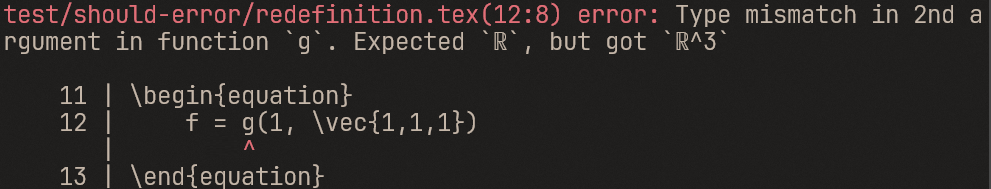
\includegraphics[scale=0.5]{./Imagens/error-type-mismatch.png}
    \end{center}
\end{figure}


\begin{codigo}[H]
    \caption{\small Validação de parâmetros de uma função.}
    \label{cod-parametros-validation}
\begin{lstlisting}[language=C, numbers=none, frame=none, inputencoding=latin1]
// ...
parameter_types := [dynamic]^Type{}
scope_enter(fn_sym.scope) {
    for &parameter in fn.parameters {
        parameter_key := key_from_identifier(parameter)
        ty := infer_type(parameter, true, ty_number)
        parameter_sym.type = ty
        append(&parameter_types, ty)
    }
}
// ...
\end{lstlisting}
\end{codigo}

%
% \begin{codigo}[htb]
%     \caption{\small Gerenciamento de escopo na validação do corpo da função.}
%     \label{cod-scope-management}
% \begin{lstlisting}[language=C, numbers=none, frame=none, inputencoding=latin1]
% scope_enter(fn_sym.scope) {
%     // Validação do corpo da função
%     check_expr(body)
%     // Inferência e validação de tipo
%     body_type := infer_type(body)
% }
% \end{lstlisting}
% \end{codigo}

%
% \begin{codigo}[htb]
%     \caption{\small .}
%     \label{cod-types-structs}
% \begin{lstlisting}[language=C, numbers=none, frame=none, inputencoding=utf8]
% case ^Decl_Equation:
%     check_decl(s)
%
% scope_enter(fn_sym.scope) {
%     // Validação do corpo da função
%     check_expr(body)
%     // Inferência e validação de tipo
%     body_type := infer_type(body)
%     result_types := [dynamic]^Type{body_type}
%     fn_type := make_function_type(parameter_types[:], result_types[:])
% }
% \end{lstlisting}
% \end{codigo}



\chapter{Resultados}
\label{chapter.resultados}


Este capítulo apresenta os resultados dos experimentos com diferentes BRDFs, servindo como validação e visualização da capacidade do compilador desenvolvido. A escolha de cada BRDF foi direcionada para explorar expressões matemáticas com diversos níveis de complexidade, aspectos importante para testar a capacidade do compilador desenvolvido neste projeto.

Os experimentos seguem uma metodologia padronizada. Inicialmente, apresenta-se a BRDF do experimento, incluindo sua referência, quando relevante e uma breve explicação conceitual. Em seguida, demonstra-se o código-fonte que descreve a BRDF em \texttt{EquationLang}, acompanhado de sua representação em PDF \LaTeX{}. Utilizando o compilador desenvolvido, o código-fonte é traduzido para linguagem de \textit{shading} GLSL e carregado na ferramenta Disney BRDF Explorer.

A análise inclui gráficos 3D e 2D da distribuição de reflexão especular e difusa da BRDF. Para demonstrar a eficácia do código GLSL gerado, são renderizados três objetos tridimensionais utilizando técnicas de \textit{ray tracing} fornecidas pela ferramenta Disney. Os objetos possuem ângulos em coordenadas polares fixas, com condições padronizadas de iluminação: ângulos de elevação ($\theta_i$) e azimutal ($\phi_i$) da luz incidente predefinidos em $33,8941$ e $145,826$ respectivamente; gamma fixado em $2,112$ e exposição em $-1,248$.
% Adicionalmente, apresenta-se o efeito da BRDF em uma esfera com renderização projetiva padrão.

O \textit{plot}\footnote{O termo \textit{plot} é comumente usado em ferramentas de visualização e análise para se referir a gráficos ou representações visuais de dados. Aqui, refere-se a representações 2D (polar) ou 3D usadas para ilustrar os componentes especular e difuso de cada canal de cor da BRDF.} 3D de BRDFs na ferramenta Disney Explorer oferece uma visualização que fixa uma direção de luz incidente ($\omega_i$) e coleta valores da direções de visualização ($\omega_o$) em um hemisfério como entrada para BRDF. Para cada direção de visualização, renderiza-se um primitivo proporcional ao valor da função BRDF.

O \textit{plot} polar, por sua vez, representa um corte bidimensional, fixando a direção de luz incidente ($\omega_i$) e o ângulo azimutal de saída ($\phi_o$), variando apenas o ângulo polar de saída ($\theta_o$), similar ao mostrado nas figuras da \autoref{brdfmodels}. Cada ponto representa o valor médio das componentes da BRDF, visualizando o comportamento da refletância em diferentes ângulos de observação. Em alguns casos, fatores logarítmicos são utilizados para melhor visualização do gráfico.

É importante observar que os gráficos polares e 3D representam simultaneamente os três canais de cores, como na \autoref{fig-ashikhmin-shirley-alternative-plots}, podendo haver sobreposição entre vermelho, azul e verde na visualização, já que a distribuição de cada canal pode ser idêntica em um dado experimento.

% Embora os experimentos contenha uma explicação sobre a BRDF, o foco principal permanece na representação fidedigna das equações em GLSL provida pelo compilador. 
% E Ainda, toda explicação que esteja fora do ambiente equatio é ignorada pelo compilaodr, então realmente é apensar para ilustrar a compilação de um arquivo por completo, por isso incluimos as explicações rudimentares ( muitos vezes em inles) para demonstrar isso. Recomenda-se observar rapidamente o código gerado para compreender sua estrutura, reconhecendo que o código GLSL gerado por computador não é tão legível quanto código \textit{shading} escrito manualmente.

Embora os experimentos contenham uma explicação sobre a BRDF, o foco principal permanece na representação fidedigna das equações em GLSL fornecida pelo compilador. Além disso, qualquer explicação presente no arquivo de entrada (\verb".tex") que esteja fora do ambiente \texttt{equation} é ignorada pelo compilador, sendo incluída apenas para ilustrar a compilação de um arquivo completo. Por essa razão, inserimos explicações rudimentares (muitas vezes em inglês) para demonstrar esse aspecto. Recomenda-se observar rapidamente o código gerado para compreender sua estrutura, reconhecendo que o código GLSL gerado pelo computador não é tão legível quanto o código \textit{shading} escrito manualmente.

Alguns experimentos exploram múltiplas formas de expressar a mesma BRDF, não apenas com parâmetros distintos, mas também com expressões matemáticas alternativas. Para facilitar a navegação, a \autoref{table-experiments} é disponibilizada para acesso rápido às imagens e códigos dos experimentos.



\begin{table}[H]
\centering
\begin{tabular}{|l|c|c|c|c|c|}
\hline
    \textbf{Experimento} & \textbf{Seção}                                            & \textbf{Equações}                                                & \textbf{Objetos 3D}                                       & \textbf{\textit{Plots}}                                  & \textbf{GLSL}  \\ \hline
    Blinn-Phong          &\autoref{section-experiment-blinn-phong}                   & \autoref{fig-blinn-phong-eqlang-latex}                           & \autoref{fig-blinn-phong-eqlang}                          & \autoref{fig-blinn-phong-plots}                          &                  \autoref{cod-blinn-phong-glsl-pt-1}              \\ \hline
    Cook-Torrance        &\autoref{sec:cook-torrance}                 & \autoref{fig-cook-torrance-eqlang-latex}                         & \autoref{fig-cook-torrance-eqlang}                        & \autoref{fig-cook-torrance-plots}                        &             \autoref{cod-cook-torrance-glsl-pt-1}              \\ \hline
    Ward                 &\autoref{section-experiment-ward}                          & \autoref{fig-ward-eqlang-latex}                                  & \autoref{fig-ward-objetcs}                                & \autoref{fig-ward-plots}                                 &                     \autoref{cod-ward-glsl-pt-1}               \\ \hline
    Ashikhmin-Shirley    &\autoref{sec:ashikhmin-shirley}             & \autoref{fig-ashikhmin-shirley-close-to-original-eqlang-latex}   & \autoref{fig-ashikhmin-shirley-close-to-original-eqlang}  & \autoref{fig-ashikhmin-shirley-close-to-original-plots}  &                  \autoref{cod-ashikhmin-shirley-close-to-original-glsl-pt-1}              \\ \hline
    Oren-Nayar           &\autoref{section-experiment-oren-nayar}                    & \autoref{fig-oren-nayar-eqlang-latex}                            & \autoref{fig-oren-nayar-eqlang}                           & \autoref{fig-oren-nayar-plots}                           &                \autoref{cod-oren-nayar-glsl-pt-1}              \\ \hline
    Ashikhmin-Shirley$_2$&\autoref{section-experiment-ashikhmin-shirley-alternative} & \autoref{fig-ashikhmin-shirley-alternative-eqlang-latex}         & \autoref{fig-ashikhmin-shirley-alternative-eqlang}        & \autoref{fig-ashikhmin-shirley-alternative-plots}        &                  \autoref{cod-ashikhmin-shirley-alternative-glsl-pt-1}              \\ \hline
    Cook-torrance$_2$    &\autoref{section-experiment-cook-torrance-alternative}     & \autoref{fig-cook-torrance-alternative-eqlang-latex}             & \autoref{fig-cook-torrance-alternative-eqlang}            & \autoref{fig-cook-torrance-alternative-plots}            & \autoref{cod-cook-torrance-alternative-glsl-pt-1}              \\ \hline
    Dür                  &\autoref{section-experiment-duer}                          & \autoref{fig-duer-eqlang-latex}                                  & \autoref{fig-duer-eqlang}                                 & \autoref{fig-duer-plots}                                 &                      \autoref{cod-duer-glsl-pt-1}              \\ \hline
    Edwards-2006         &\autoref{section-experiment-edwards-2006}                  & \autoref{fig-edwards-2006-eqlang-latex}                          & \autoref{fig-edwards-2006-eqlang}                         & \autoref{fig-edwards-2006-plots}                         &              \autoref{cod-edwards-2006-glsl-pt-1}              \\ \hline
    Kajiya-Kay-1989$_*$  &\autoref{section-experiment-kajiya}                        & \autoref{fig-kajiya-eqlang-latex}                                & \autoref{fig-kajiya-objects}                              & \autoref{fig-kajiya-plots}                               &                  \autoref{cod-kajiya-glsl-pt-1}              \\ \hline
    Minnaert             &\autoref{section-experiment-minnaert}                      & \autoref{fig-minnaert-eqlang-latex}                              & \autoref{fig-minnaert-eqlang}                             & \autoref{fig-minnaert-plots}                             &                  \autoref{cod-minnaert-glsl-pt-1}              \\ \hline
\end{tabular}
\caption{Tabela dos Experimentos.}
\label{table-experiments}
\end{table}


%%%
Concluímos que os experimentos realizados apresentaram resultados satisfatórios. O compilador desenvolvido demonstra flexibilidade ao capturar as nuances das diferentes BRDFs, inclusive em materiais com estruturas complexas. O sistema permite diversas parametrizações e equações alternativas para representar os comportamentos da superfície.

Os resultados obtidos não apenas validam a metodologia adotada, mas também abrem perspectivas para futuras extensões e refinamentos da ferramenta. Após o último experimento, seguimos diretamente para o capítulo de conclusão (\autoref{chapter-conclusion}), onde são discutidas as possíveis direções para a continuidade deste trabalho.



\section{Experimento BRDF Blinn-Phong} \label{section-experiment-blinn-phong}

Neste experimento usamos uma BRDF com um método simplificado de cálculo de reflexão especular, presente na \autoref{fig-blinn-phong-eqlang-latex}, introduzido por Blinn-Phong \cite{blinn1977models}. O \autoref{cod-blinn-phong-eqlang}, escrito \texttt{EquationLang}, é a entrada para o compilador. O \autoref{cod-blinn-phong-glsl-pt-1} e \autoref{cod-blinn-phong-glsl-pt-2} são a sáida em GLSL. A renderização dos objetos 3D estão em \autoref{fig-blinn-phong-eqlang}. Por fim, os \textit{plots} estão na \autoref{fig-blinn-phong-plots}.

%%%%%%%%%%%%%%%%%%%%%%%%%%%%%%%%%%%%%%%%%%%%%%%%%
\subsection{Representação em documento \LaTeX{}}
%%%%%%%%%%%%%%%%%%%%%%%%%%%%%%%%%%%%%%%%%%%%%%%%%
\begin{figure}[H]
    \caption{\label{fig-blinn-phong-eqlang-latex} 
    \small Equações da BRDF do experimento Blinn-Phong em documento \LaTeX{}.}
    \begin{center}
        % 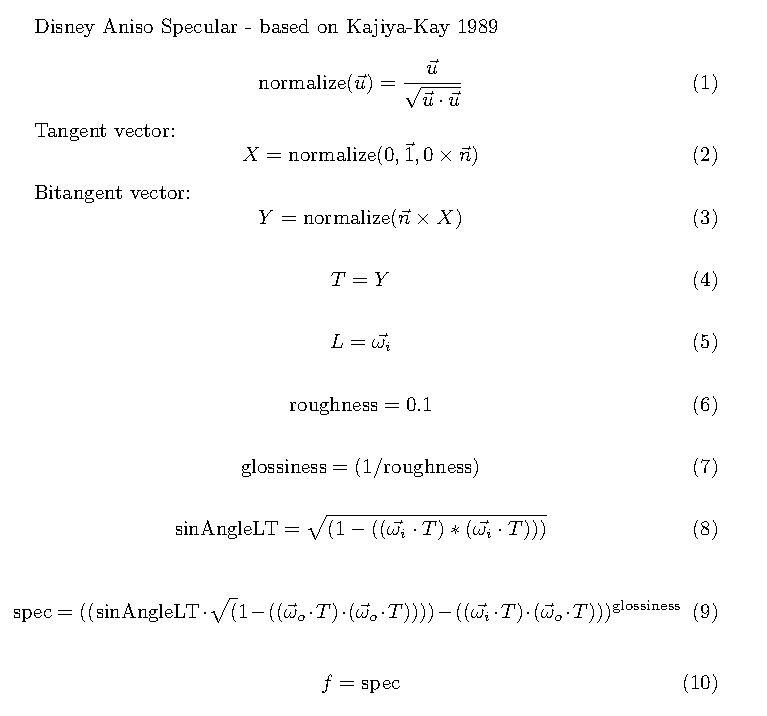
\includegraphics[scale=1.1,width=\textwidth]{./Imagens/brdfs/aniso.pdf}
        
\includegraphics[scale=0.92]{./Imagens/brdfs/blinn-phong.pdf}
    \end{center}
\end{figure}


%%%%%%%%%%%%%%%%%%%%%%%%%%%%%%%%%%%%%%%%%%%%%%%%%
\subsection{Código Fonte em \texttt{EquationLang}}
%%%%%%%%%%%%%%%%%%%%%%%%%%%%%%%%%%%%%%%%%%%%%%%%%
\begin{codigo}[H]
    \caption{\small Código fonte da BRDF do experimento Blinn-Phong.}
    \label{cod-blinn-phong-eqlang}
\begin{lstlisting}[language=tex, frame=none, inputencoding=utf8]
\begin{equation}
    \rho_{d} = \vec{0,1,1}
\end{equation}

\begin{equation}
    \rho_{s} = \vec{1,0,1}
\end{equation}

\begin{equation}
    n = +2^8
\end{equation}

\begin{equation}
f = \frac{\rho_{d}}{\pi} + \rho_{s} * \frac{n+2}{2*\pi} *
\cos{\theta_{h}}^{n}
\end{equation}
\end{lstlisting}
\end{codigo}

%%%%%%%%%%%%%%%%%%%%%%%%%%%%%%%%%%%%%%%%%%%%%%%%%
\subsection{Código GLSL Gerado}
%%%%%%%%%%%%%%%%%%%%%%%%%%%%%%%%%%%%%%%%%%%%%%%%%
\begin{codigo}[H]
    \caption{\small Saída do compilador: código GLSL da BRDF do experimento Blinn-Phong (parte 1 de 2).}
    \label{cod-blinn-phong-glsl-pt-1}
\begin{lstlisting}[language=C, inputencoding=utf8]
analytic ::begin parameters
#[type][name][min val][max val][default val]
::end parameters
::begin shader
//////////// START OF BUILTINS DECLARTION ////////////
vec3 var_0_vec_h;
vec3 var_3_vec_n;
float var_10_theta_h;
float var_11_theta_d;
float var_1_pi;
float var_2_epsilon;
vec3 var_4_vec_omega_i;
float var_5_theta_i;
float var_6_phi_i;
vec3 var_7_vec_omega_o;
float var_8_theta_o;
float var_9_phi_o;
//////////// END OF BUILTINS DECLARTION ////////////
//////////// START OF USER DECLARED ////////////
vec3 var_12_rho_s;
float var_13_n;
vec3 var_14_rho_d;
vec3 var_15_f;
//////////// END OF USER DECLARED ////////////
\end{lstlisting}
\end{codigo}

\begin{codigo}[H]
    \caption{\small Saída do compilador: código GLSL da BRDF do experimento Blinn-Phong (parte 2 de 2).}
    \label{cod-blinn-phong-glsl-pt-2}
\begin{lstlisting}[language=C, inputencoding=utf8]
vec3 BRDF(vec3 L, vec3 V, vec3 N, vec3 X, vec3 Y) {
  //////////// START OF BUILTINS INITIALIZATION ////////////
  var_0_vec_h = normalize(L + V);
  var_3_vec_n = normalize(N);
  var_1_pi = 3.141592653589793;
  var_2_epsilon = 1.192092896e-07;
  var_4_vec_omega_i = L;
  var_5_theta_i = atan(var_4_vec_omega_i.y, var_4_vec_omega_i.x);
  var_6_phi_i = atan(sqrt(var_4_vec_omega_i.y * var_4_vec_omega_i.y +
                          var_4_vec_omega_i.x * var_4_vec_omega_i.x),
                     var_4_vec_omega_i.z);
  var_7_vec_omega_o = V;
  var_8_theta_o = atan(var_7_vec_omega_o.y, var_7_vec_omega_o.x);
  var_9_phi_o = atan(sqrt(var_7_vec_omega_o.y * var_7_vec_omega_o.y +
                          var_7_vec_omega_o.x * var_7_vec_omega_o.x),
                     var_7_vec_omega_o.z);
  var_10_theta_h = acos(dot(var_0_vec_h, N));
  var_11_theta_d = acos(dot(var_0_vec_h, var_4_vec_omega_i));
  //////////// END OF BUILTINS INITIALIZATION ////////////
  var_12_rho_s = vec3(1.0, 0.0, 1.0);
  var_13_n = pow(2.0, 8.0);
  var_14_rho_d = vec3(0.0, 1.0, 1.0);
  var_15_f = ((var_14_rho_d / var_1_pi) +
              ((var_12_rho_s * ((var_13_n + 2.0) / (2.0 * var_1_pi))) *
               pow(cos(var_10_theta_h), var_13_n)));

  return vec3(var_15_f);
}
\end{lstlisting}
\end{codigo}

%%%%%%%%%%%%%%%%%%%%%%%%%%%%%%%%%%%%%%%%%%%%%%%%%
\subsection{Visualização do Resultado}
%%%%%%%%%%%%%%%%%%%%%%%%%%%%%%%%%%%%%%%%%%%%%%%%%

\begin{figure}[H]
  
    \caption{\small{\textit{Plots} da distribuição de reflexão especular e difusa do experimento Blinn-Phong.}}
    \label{fig-blinn-phong-plots}
\minipage{0.48\textwidth}
    \vspace{42px}
  
\includegraphics[width=\linewidth]{./Imagens/brdfs/blinn-phong-3D-plot}
    % \caption{\small{(a)}}\label{fig:awesome_image1}
    % \vspace{0.1px}
    \legend{ \small (a) 3D \textit{plot}}
\endminipage\hfill
\minipage{0.48\textwidth}
  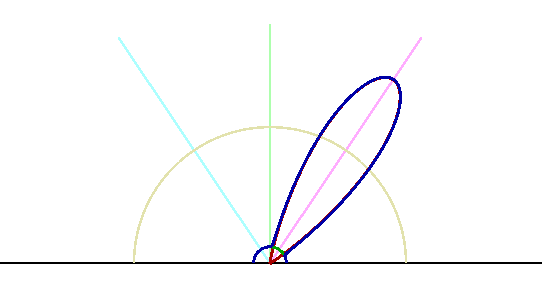
\includegraphics[width=\linewidth]{./Imagens/brdfs/blinn-phong-polar-plot-log.png}
    \legend{ \small (b) \textit{Polar plot}}
    % \caption{\small{(b)}}\label{fig:awesome_image1}
\endminipage\hfill
\end{figure}

\begin{figure}[H]
    \caption{\small{Objetos 3D renderizados pelo experimento Blinn-Phong.}}
    \label{fig-blinn-phong-eqlang}
\minipage{0.32\textwidth}
  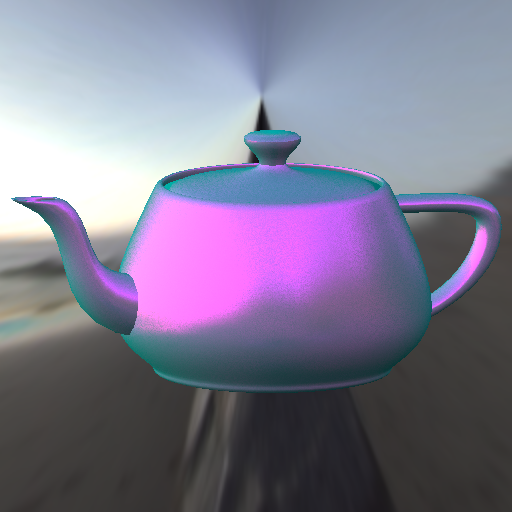
\includegraphics[width=\linewidth]{./Imagens/brdfs/blinn-phong-teapot.png}
    \legend{ \small (a) \textit{Teapot}}
\endminipage\hfill
\minipage{0.32\textwidth}
  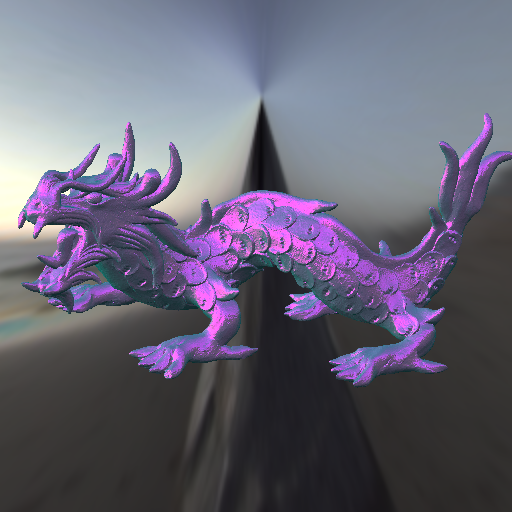
\includegraphics[width=\linewidth]{./Imagens/brdfs/blinn-phong-dragon.png}
    \legend{ \small (b) Dragão de Stanford}
\endminipage\hfill
\minipage{0.32\textwidth}%
  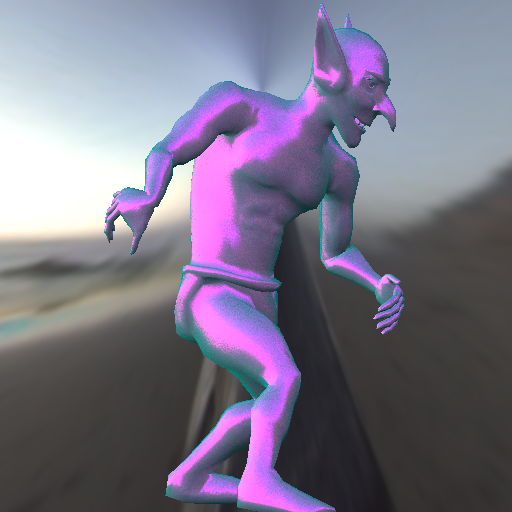
\includegraphics[width=\linewidth]{./Imagens/brdfs/blinn-phong-goblin.png}
    \legend{ \small (c) Goblin}
\endminipage
\end{figure}


\section{Experimento BRDF Cook-Torrance}\label{sec:cook-torrance}

Este experimento é baseada no modelo microfacetado que descreve o comportamento de reflexão de superfícies metálicas descrito no trabalho de Cook-Torrance \cite{cook1982reflectance}. As equações e parametros escolhidos que descrevem esse modelo estão em \autoref{fig-cook-torrance-eqlang-latex}. O código fonte em \texttt{EquationLang} para o compilador está em \autoref{cod-cook-torrance-eqlang}. O código GLSL está dividido em duas partes, parte 1 está no \autoref{cod-cook-torrance-glsl-pt-1} e a segunda parte está em \autoref{cod-cook-torrance-glsl-pt-2}. A renderização dos objetos 3D usando essa BRDF se encontra em \autoref{fig-cook-torrance-eqlang}. Usamos plot logaritmo para gerar os plots 3D e polar presentes na \autoref{fig-cook-torrance-plots}.

%%%%%%%%%%%%%%%%%%%%%%%%%%%%%%%%%%%%%%%%%%%%%%%%%
\subsection{Representação em documento \LaTeX{}}
%%%%%%%%%%%%%%%%%%%%%%%%%%%%%%%%%%%%%%%%%%%%%%%%%
\begin{figure}[H]
    \caption{\label{fig-cook-torrance-eqlang-latex} \small Equações da BRDF do experimento cook-torrance em documento \LaTeX{}.}
    \begin{center}
        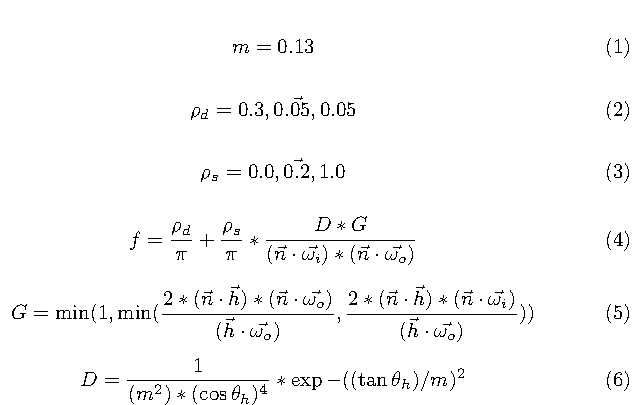
\includegraphics[scale=0.92]{./Imagens/brdfs/cook-torrance.pdf}
    \end{center}
\end{figure}

%%%%%%%%%%%%%%%%%%%%%%%%%%%%%%%%%%%%%%%%%%%%%%%%%
\subsection{Visualização do Resultado}
%%%%%%%%%%%%%%%%%%%%%%%%%%%%%%%%%%%%%%%%%%%%%%%%%
\begin{figure}[H]
    \caption{\small{Distribuição de Reflexão Especular e Difusa da BRDF}}\label{fig-cook-torrance-plots}
\minipage{0.48\textwidth}
    \vspace{42px}
  
\includegraphics[width=\linewidth]{./Imagens/brdfs/cook-torrance-3D-plot}
    % \vspace{0.1px}
    \legend{ \small (a) 3D \textit{plot}}
\endminipage\hfill
\minipage{0.48\textwidth}
  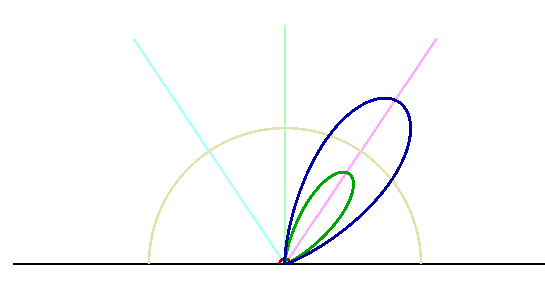
\includegraphics[width=\linewidth]{./Imagens/brdfs/cook-torrance-polar-plot-log.png}
    \legend{ \small (b) \textit{Polar plot}}
\endminipage\hfill
\end{figure}

\begin{figure}[H]
    \caption{\small{Objetos 3D renderizados por este experimento}}\label{fig-cook-torrance-eqlang}
\minipage{0.32\textwidth}
  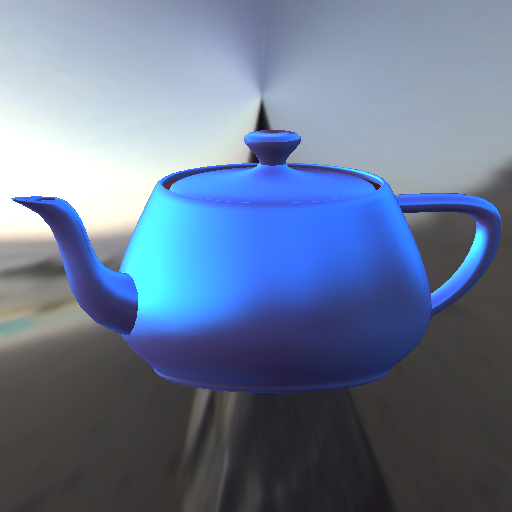
\includegraphics[width=\linewidth]{./Imagens/brdfs/cook-torrance-teapot.png}
    \legend{ \small (a) \textit{Teapot}}
\endminipage\hfill
\minipage{0.32\textwidth}
  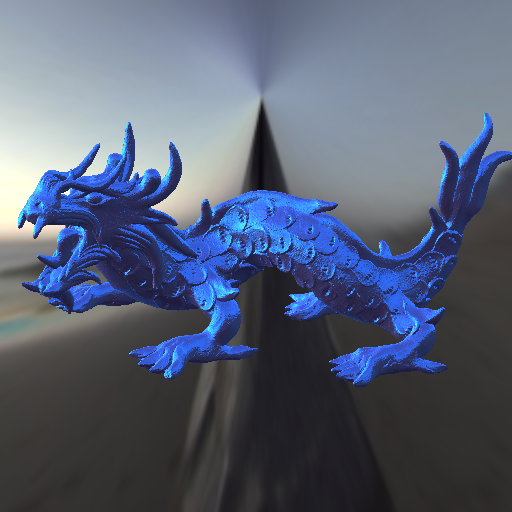
\includegraphics[width=\linewidth]{./Imagens/brdfs/cook-torrance-dragon.png}
    \legend{ \small (b) Dragão de Stanford}
\endminipage\hfill
\minipage{0.32\textwidth}%
  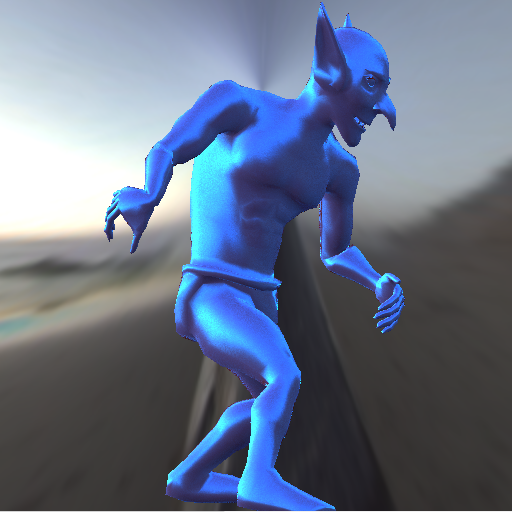
\includegraphics[width=\linewidth]{./Imagens/brdfs/cook-torrance-goblin.png}
    \legend{ \small (c) Goblin}
\endminipage
\end{figure}

%%%%%%%%%%%%%%%%%%%%%%%%%%%%%%%%%%%%%%%%%%%%%%%%%
\subsection{Código GLSL Gerado}
%%%%%%%%%%%%%%%%%%%%%%%%%%%%%%%%%%%%%%%%%%%%%%%%%
\begin{codigo}[H]
    \caption{\small Saida do compilador, código GLSL da BRDF deste experimento (parte 1). }
    \label{cod-cook-torrance-glsl-pt-1}
\begin{lstlisting}[language=C, inputencoding=utf8]
analytic ::begin parameters
#[type][name][min val][max val][default val]
::end parameters
::begin shader
//////////// START OF BUILTINS DECLARTION ////////////
vec3 var_0_vec_h;
vec3 var_3_vec_n;
float var_10_theta_h;
float var_11_theta_d;
float var_1_pi;
float var_2_epsilon;
vec3 var_4_vec_omega_i;
float var_5_theta_i;
float var_6_phi_i;
vec3 var_7_vec_omega_o;
float var_8_theta_o;
float var_9_phi_o;
//////////// END OF BUILTINS DECLARTION ////////////
//////////// START OF USER DECLARED ////////////
float var_12_G;
vec3 var_13_rho_s;
float var_14_m;
float var_15_D;
vec3 var_16_rho_d;
vec3 var_17_f;
//////////// END OF USER DECLARED ////////////
//////////// START FUNCTIONS DECLARATIONS ////////////
//////////// END FUNCTIONS DECLARATIONS ////////////
\end{lstlisting}
\end{codigo}

\begin{codigo}[H]
    \caption{\small Saida do compilador, código GLSL da BRDF deste experimento  (parte 2). }
    \label{cod-cook-torrance-glsl-pt-2}
\begin{lstlisting}[language=C, inputencoding=utf8]
vec3 BRDF(vec3 L, vec3 V, vec3 N, vec3 X, vec3 Y) {

  //////////// START OF BUILTINS INITIALIZATION ////////////
  var_0_vec_h = normalize(L + V);
  var_3_vec_n = normalize(N);
  var_1_pi = 3.141592653589793;
  var_2_epsilon = 1.192092896e-07;
  var_4_vec_omega_i = L;
  var_5_theta_i = atan(var_4_vec_omega_i.y, var_4_vec_omega_i.x);
  var_6_phi_i = atan(sqrt(var_4_vec_omega_i.y * var_4_vec_omega_i.y +
                          var_4_vec_omega_i.x * var_4_vec_omega_i.x),
                     var_4_vec_omega_i.z);
  var_7_vec_omega_o = V;
  var_8_theta_o = atan(var_7_vec_omega_o.y, var_7_vec_omega_o.x);
  var_9_phi_o = atan(sqrt(var_7_vec_omega_o.y * var_7_vec_omega_o.y +
                          var_7_vec_omega_o.x * var_7_vec_omega_o.x),
                     var_7_vec_omega_o.z);
  var_10_theta_h = acos(dot(var_0_vec_h, N));
  var_11_theta_d = acos(dot(var_0_vec_h, var_4_vec_omega_i));
  //////////// END OF BUILTINS INITIALIZATION ////////////

  var_12_G = min(1.0, min((((2.0 * (dot(var_3_vec_n, var_0_vec_h))) *
                            (dot(var_3_vec_n, var_7_vec_omega_o))) /
                           (dot(var_0_vec_h, var_7_vec_omega_o))),
                          (((2.0 * (dot(var_3_vec_n, var_0_vec_h))) *
                            (dot(var_3_vec_n, var_4_vec_omega_i))) /
                           (dot(var_0_vec_h, var_7_vec_omega_o)))));
  var_13_rho_s = vec3(0.0, 0.2, 1.0);
  var_14_m = 0.13;
  var_15_D = ((1.0 / ((pow(var_14_m, 2.0)) * pow((cos(var_10_theta_h)), 4.0))) *
              exp((-pow((((tan(var_10_theta_h)) / var_14_m)), 2.0))));
  var_16_rho_d = vec3(0.3, 0.05, 0.05);
  var_17_f =
      ((var_16_rho_d / var_1_pi) +
       ((var_13_rho_s / var_1_pi) *
        ((var_15_D * var_12_G) / ((dot(var_3_vec_n, var_4_vec_omega_i)) *
                                  (dot(var_3_vec_n, var_7_vec_omega_o))))));

  return vec3(var_17_f);
}
\end{lstlisting}
\end{codigo}

%%%%%%%%%%%%%%%%%%%%%%%%%%%%%%%%%%%%%%%%%%%%%%%%%
\subsection{Código Fonte em \texttt{EquationLang}}
%%%%%%%%%%%%%%%%%%%%%%%%%%%%%%%%%%%%%%%%%%%%%%%%%
\begin{codigo}[H]
    \caption{\small Código fonte da BRDF deste experimento.}
    \label{cod-cook-torrance-eqlang}
\begin{lstlisting}[language=tex, frame=none, inputencoding=utf8]
\begin{equation}
m = 0.13
\end{equation}

\begin{equation}
    \rho_{d} = \vec{0.3,0.05,0.05}
\end{equation}

\begin{equation}
    \rho_{s} = \vec{0.0,0.2,1.0}
\end{equation}

\begin{equation}
f = \frac{\rho_{d}}{\pi} +
\frac{\rho_{s}}{\pi} *
\frac{D*G}{({\vec{n}}\cdot{\vec{\omega_{i}}}) *
({\vec{n}}\cdot{\vec{\omega_{o}}})}
\end{equation}

\begin{equation}
G = \min(1,\min(
\frac{2 *
({\vec{n}}\cdot{\vec{h}}) *
({\vec{n}}\cdot{\vec{\omega_{o}}})
}
{({\vec{h}}\cdot{\vec{\omega_{o}}})},
\frac{2 *
({\vec{n}}\cdot{\vec{h}}) *
({\vec{n}}\cdot{\vec{\omega_{i}}})
}
{({\vec{h}}\cdot{\vec{\omega_{o}}})}
))
\end{equation}

\begin{equation}
D = \frac{1}
{(m^{2}) * (\cos{\theta_{h}})^{4}} *
\exp{-((\tan{\theta_{h}})/m)^{2}}
\end{equation}
\end{lstlisting}
\end{codigo}


\section{Experimento BRDF Ward} \label{section-experiment-ward}

Este experimento é baseado na BRDF revisada segundo as notas de Walter \cite{walter2005notes}, que detalham o modelo de Ward. Suas equações podem ser vistas na \autoref{fig-ward-eqlang-latex}, enquanto o código em \texttt{EquationLang} está disponível no \autoref{cod-ward-eqlang-pt-1} (parte 1) e no \autoref{cod-ward-eqlang-pt-2} (parte 2). O código gerado pelo compilador é formado pelo \autoref{cod-ward-glsl-pt-1} e pelo \autoref{cod-ward-glsl-pt-2}. A renderização de objetos usando este modelo é ilustrada na \autoref{fig-ward-objetcs}, e os \textit{plots} da sua refletância estão na \autoref{fig-ward-plots}.
%%


%%%%%%%%%%%%%%%%%%%%%%%%%%%%%%%%%%%%%%%%%%%%%%%%%
\subsection{Representação em documento \LaTeX{}}
%%%%%%%%%%%%%%%%%%%%%%%%%%%%%%%%%%%%%%%%%%%%%%%%%
\begin{figure}[H]
    \caption{\label{fig-ward-eqlang-latex} \small Equações da BRDF do experimento Ward em documento \LaTeX{}.}
    \begin{center}
        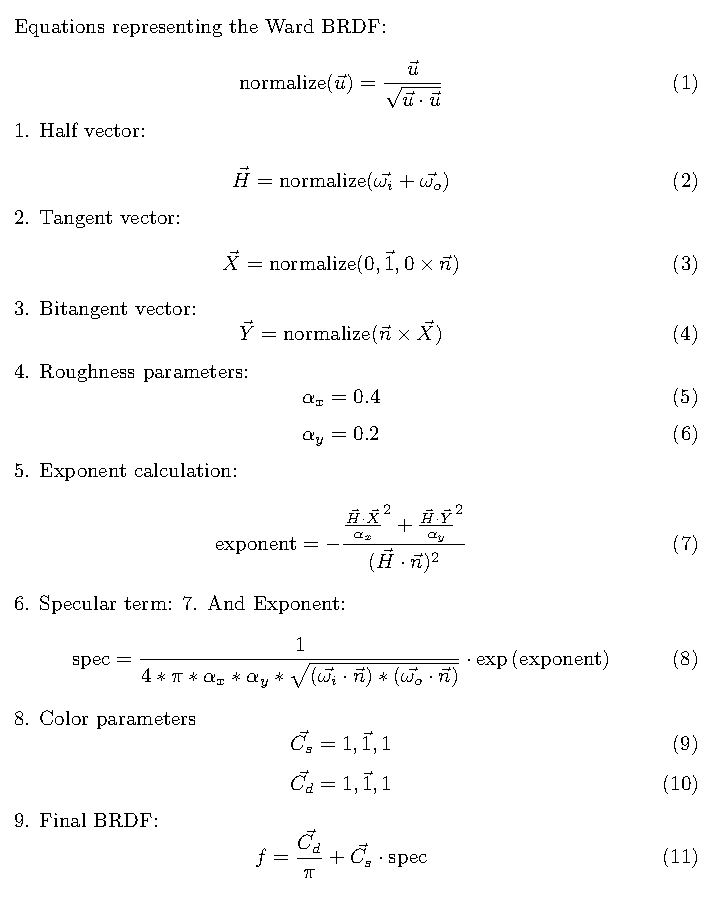
\includegraphics[scale=0.92]{./Imagens/brdfs/ward.pdf}
    \end{center}
\end{figure}

%%%%%%%%%%%%%%%%%%%%%%%%%%%%%%%%%%%%%%%%%%%%%%%%%
\subsection{Código Fonte em \texttt{EquationLang}}
%%%%%%%%%%%%%%%%%%%%%%%%%%%%%%%%%%%%%%%%%%%%%%%%%
\begin{codigo}[H]
    \caption{\small Código fonte da BRDF do experimento Ward (parte 1 de 2).}
    \label{cod-ward-eqlang-pt-1}
\begin{lstlisting}[language=tex, frame=none, inputencoding=utf8]
Equations representing the Ward BRDF:
   \begin{equation}
      \text{normalize}(\vec{u}) = \frac{\vec{u}}{\sqrt{\vec{u} \cdot \vec{u}}}
   \end{equation}
1. Half vector:
   \begin{equation}
   \vec{H} = \text{normalize}(\vec{\omega_i} + \vec{\omega_o})
   \end{equation}
2. Tangent vector:
   \begin{equation}
   \vec{X} = \text{normalize}(\vec{0,1,0} \times \vec{n})
   \end{equation}
3. Bitangent vector:
   \begin{equation}
   \vec{Y} = \text{normalize}(\vec{n} \times \vec{X})
   \end{equation}
4. Roughness parameters:
   \begin{equation}
   \alpha_x = 0.4
   \end{equation}
   \begin{equation}
   \alpha_y = 0.2
   \end{equation}
\end{lstlisting}
\end{codigo}

\begin{codigo}[H]
    \caption{\small Código fonte da BRDF do experimento Ward (parte 2 de 2).}
    \label{cod-ward-eqlang-pt-2}
\begin{lstlisting}[language=tex, frame=none, inputencoding=utf8]
5. Exponent calculation:
   \begin{equation}
   \text{exponent} = -\frac{
       \frac{\vec{H} \cdot \vec{X}}{\alpha_x}^2 +
       \frac{\vec{H} \cdot \vec{Y}}{\alpha_y}^2
   }{(\vec{H} \cdot \vec{n})^2}
   \end{equation}
6. Specular term:
7. And Exponent:
   \begin{equation}
   \text{spec} = \frac{1}{4*\pi * \alpha_x *\alpha_y *\sqrt{(\vec{\omega_i} \cdot \vec{n}) * (\vec{\omega_o} \cdot \vec{n})}}
      \cdot \exp{( \text{exponent} )}
   \end{equation}
8. Color parameters
   \begin{equation}
   \vec{C_s} = \vec{1, 1, 1}
   \end{equation}
   \begin{equation}
   \vec{C_d} = \vec{ 1, 1, 1 }
   \end{equation}
9. Final BRDF:
   \begin{equation}
   f = \frac{\vec{C_d}}{\pi} + \vec{C_s} \cdot \text{spec}
   \end{equation}
\end{lstlisting}
\end{codigo}

%%%%%%%%%%%%%%%%%%%%%%%%%%%%%%%%%%%%%%%%%%%%%%%%%
\subsection{Código GLSL Gerado}
%%%%%%%%%%%%%%%%%%%%%%%%%%%%%%%%%%%%%%%%%%%%%%%%%
\begin{codigo}[H]
    \caption{\small Saída do compilador: código GLSL da BRDF do experimento Ward (parte 1 de 2).}
    \label{cod-ward-glsl-pt-1}
\begin{lstlisting}[language=C, inputencoding=utf8]
analytic
::begin parameters
#[type][name][min val][max val][default val]
::end parameters
::begin shader
//////////// START OF BUILTINS DECLARTION ////////////
vec3 var_0_vec_h;
vec3 var_3_vec_n;
float var_10_theta_h;
float var_11_theta_d;
float var_1_pi;
float var_2_epsilon;
vec3 var_4_vec_omega_i;
float var_5_theta_i;
float var_6_phi_i;
vec3 var_7_vec_omega_o;
float var_8_theta_o;
float var_9_phi_o;
//////////// END OF BUILTINS DECLARTION ////////////
//////////// START OF USER DECLARED ////////////
vec3 var_14_vec_X;
vec3 var_15_vec_Y;
float var_16_alpha_x;
float var_17_alpha_y;
vec3 var_18_vec_C_d;
vec3 var_19_vec_C_s;
vec3 var_20_vec_H;
float var_21_text_exponent;
float var_22_text_spec;
vec3 var_23_f;
//////////// END OF USER DECLARED ////////////
//////////// START FUNCTIONS DECLARATIONS ////////////
vec3 var_12_text_normalize(vec3 var_13_vec_u) {
  return (var_13_vec_u / sqrt(dot(var_13_vec_u, var_13_vec_u)));
}
//////////// END FUNCTIONS DECLARATIONS ////////////
\end{lstlisting}
\end{codigo}

\begin{codigo}[H]
    \caption{\small Saída do compilador: código GLSL da BRDF do experimento Ward (parte 2 de 2).}
\label{cod-ward-glsl-pt-2}
\begin{lstlisting}[language=C, inputencoding=utf8]
vec3 BRDF(vec3 L, vec3 V, vec3 N, vec3 X, vec3 Y) {
  //////////// START OF BUILTINS INITIALIZATION ////////////
  var_0_vec_h = normalize(L + V);
  var_3_vec_n = normalize(N);
  var_1_pi = 3.141592653589793;
  var_2_epsilon = 1.192092896e-07;
  var_4_vec_omega_i = L;
  var_5_theta_i = atan(var_4_vec_omega_i.y, var_4_vec_omega_i.x);
  var_6_phi_i = atan(sqrt(var_4_vec_omega_i.y * var_4_vec_omega_i.y +
                          var_4_vec_omega_i.x * var_4_vec_omega_i.x),
                     var_4_vec_omega_i.z);
  var_7_vec_omega_o = V;
  var_8_theta_o = atan(var_7_vec_omega_o.y, var_7_vec_omega_o.x);
  var_9_phi_o = atan(sqrt(var_7_vec_omega_o.y * var_7_vec_omega_o.y +
                          var_7_vec_omega_o.x * var_7_vec_omega_o.x),
                     var_7_vec_omega_o.z);
  var_10_theta_h = acos(dot(var_0_vec_h, N));
  var_11_theta_d = acos(dot(var_0_vec_h, var_4_vec_omega_i));
  //////////// END OF BUILTINS INITIALIZATION ////////////
  var_14_vec_X = var_12_text_normalize(cross(vec3(0.0, 1.0, 0.0), var_3_vec_n));
  var_15_vec_Y = var_12_text_normalize(cross(var_3_vec_n, var_14_vec_X));
  var_16_alpha_x = 0.4;
  var_17_alpha_y = 0.2;
  var_18_vec_C_d = vec3(1.0, 1.0, 1.0);
  var_19_vec_C_s = vec3(1.0, 1.0, 1.0);
  var_20_vec_H = var_12_text_normalize((var_4_vec_omega_i + var_7_vec_omega_o));
  var_21_text_exponent = (-((pow((dot(var_20_vec_H, var_14_vec_X) / var_16_alpha_x), 2.0) +
          pow((dot(var_20_vec_H, var_15_vec_Y) / var_17_alpha_y), 2.0)) /
         pow((dot(var_20_vec_H, var_3_vec_n)), 2.0)));
  var_22_text_spec = ((1.0 / ((((4.0 * var_1_pi) * var_16_alpha_x) * var_17_alpha_y) *
               sqrt(((dot(var_4_vec_omega_i, var_3_vec_n)) *
                     (dot(var_7_vec_omega_o, var_3_vec_n)))))) *
       exp((var_21_text_exponent)));
  var_23_f = ((var_18_vec_C_d / var_1_pi) + (var_19_vec_C_s * var_22_text_spec));

  return vec3(var_23_f);
}
\end{lstlisting}
\end{codigo}

%%%%%%%%%%%%%%%%%%%%%%%%%%%%%%%%%%%%%%%%%%%%%%%%%
\subsection{Visualização do Resultado}
%%%%%%%%%%%%%%%%%%%%%%%%%%%%%%%%%%%%%%%%%%%%%%%%%
\begin{figure}[H]
    \caption{\small{\textit{Plots} da distribuição de reflexão especular e difusa do experimento Ward.}}
    \label{fig-ward-plots}

\minipage{0.48\textwidth}
    \vspace{42px}
  
\includegraphics[width=\linewidth]{./Imagens/brdfs/ward-3D-plot}
    % \vspace{0.1px}
    \legend{ \small (a) 3D \textit{plot}}
\endminipage\hfill
\minipage{0.48\textwidth}
  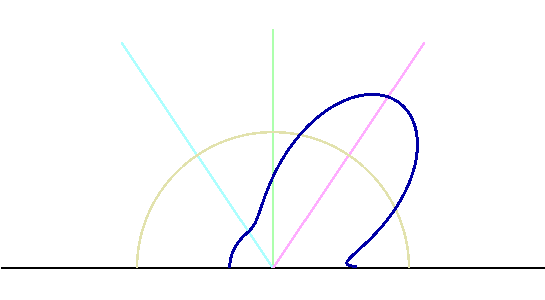
\includegraphics[width=\linewidth]{./Imagens/brdfs/ward-polar-plot.png}
    \legend{ \small (b) \textit{Polar plot}}
\endminipage\hfill
\end{figure}

\begin{figure}[H]
    \caption{\small{Objetos 3D renderizados pelo experimento Ward.}}\label{fig-ward-objetcs}
\minipage{0.32\textwidth}
  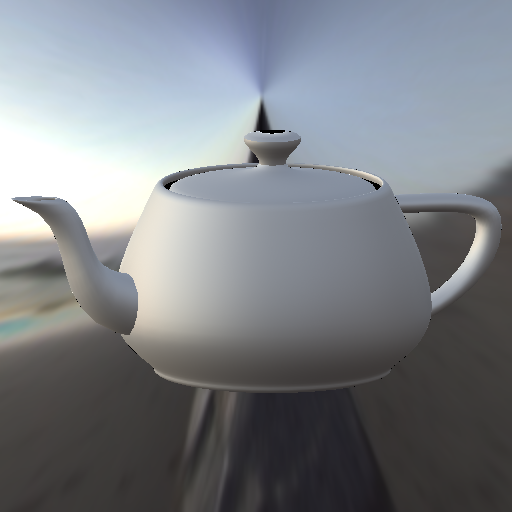
\includegraphics[width=\linewidth]{./Imagens/brdfs/ward-teapot.png}
    \legend{ \small (a) \textit{Teapot}}
\endminipage\hfill
\minipage{0.32\textwidth}
  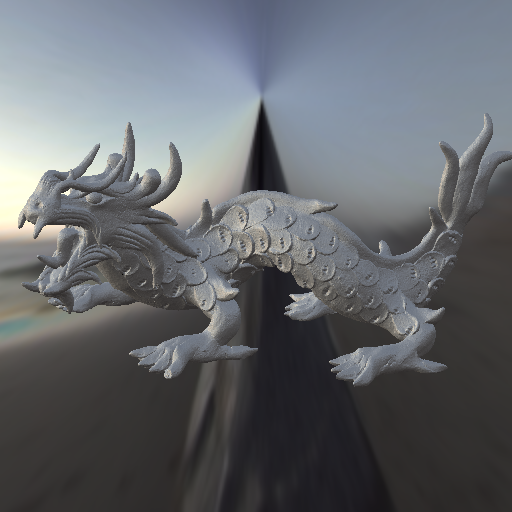
\includegraphics[width=\linewidth]{./Imagens/brdfs/ward-dragon.png}
    \legend{ \small (b) Dragão de Stanford}
\endminipage\hfill
\minipage{0.32\textwidth}%
  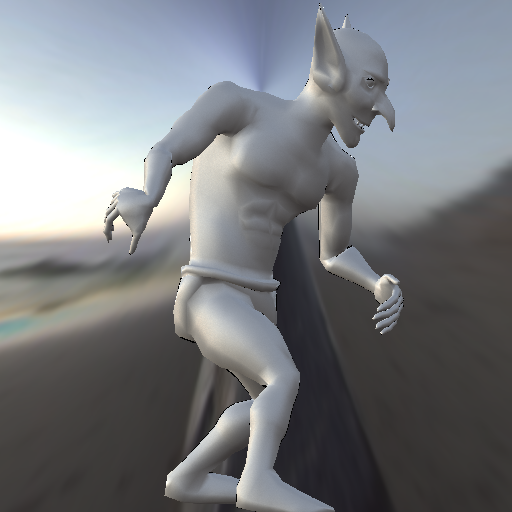
\includegraphics[width=\linewidth]{./Imagens/brdfs/ward-goblin.png}
    \legend{ \small (c) Goblin}
\endminipage
\end{figure}



\section{Experimento BRDF Ashikhmin-Shirley}\label{sec:ashikhmin-shirley}

Neste experimento, utilizamos uma BRDF anisotrópica desenvolvida por Ashikhmin-Shirley \cite{ashikhmin2000anisotropic}, que apresenta um modelo de reflexão não uniforme. A descrição matemática está presente na \autoref{fig-ashikhmin-shirley-close-to-original-eqlang-latex}, com o código-fonte em \texttt{EquationLang} disponível no \autoref{cod-ashikhmin-shirley-close-to-original-eqlang-pt-1} e no \autoref{cod-ashikhmin-shirley-close-to-original-eqlang-pt-2}. Destacamos que o compilador corretamente ignora texto fora do ambiente \texttt{equation}. O código gerado em GLSL é apresentado no \autoref{cod-ashikhmin-shirley-close-to-original-glsl-pt-1} e no \autoref{cod-ashikhmin-shirley-close-to-original-glsl-pt-2}. A renderização dos objetos 3D pode ser observada na \autoref{fig-ashikhmin-shirley-close-to-original-eqlang}, e os \textit{plots} correspondentes estão na \autoref{fig-ashikhmin-shirley-close-to-original-plots}.
%

%%%%%%%%%%%%%%%%%%%%%%%%%%%%%%%%%%%%%%%%%%%%%%%%%
\subsection{Representação em documento \LaTeX{}}
%%%%%%%%%%%%%%%%%%%%%%%%%%%%%%%%%%%%%%%%%%%%%%%%%
\begin{figure}[H]
    \caption{\label{fig-ashikhmin-shirley-close-to-original-eqlang-latex}
    \small Equações da BRDF do experimento Ashikhmin-Shirley em documento \LaTeX{}.}
    \begin{center}
        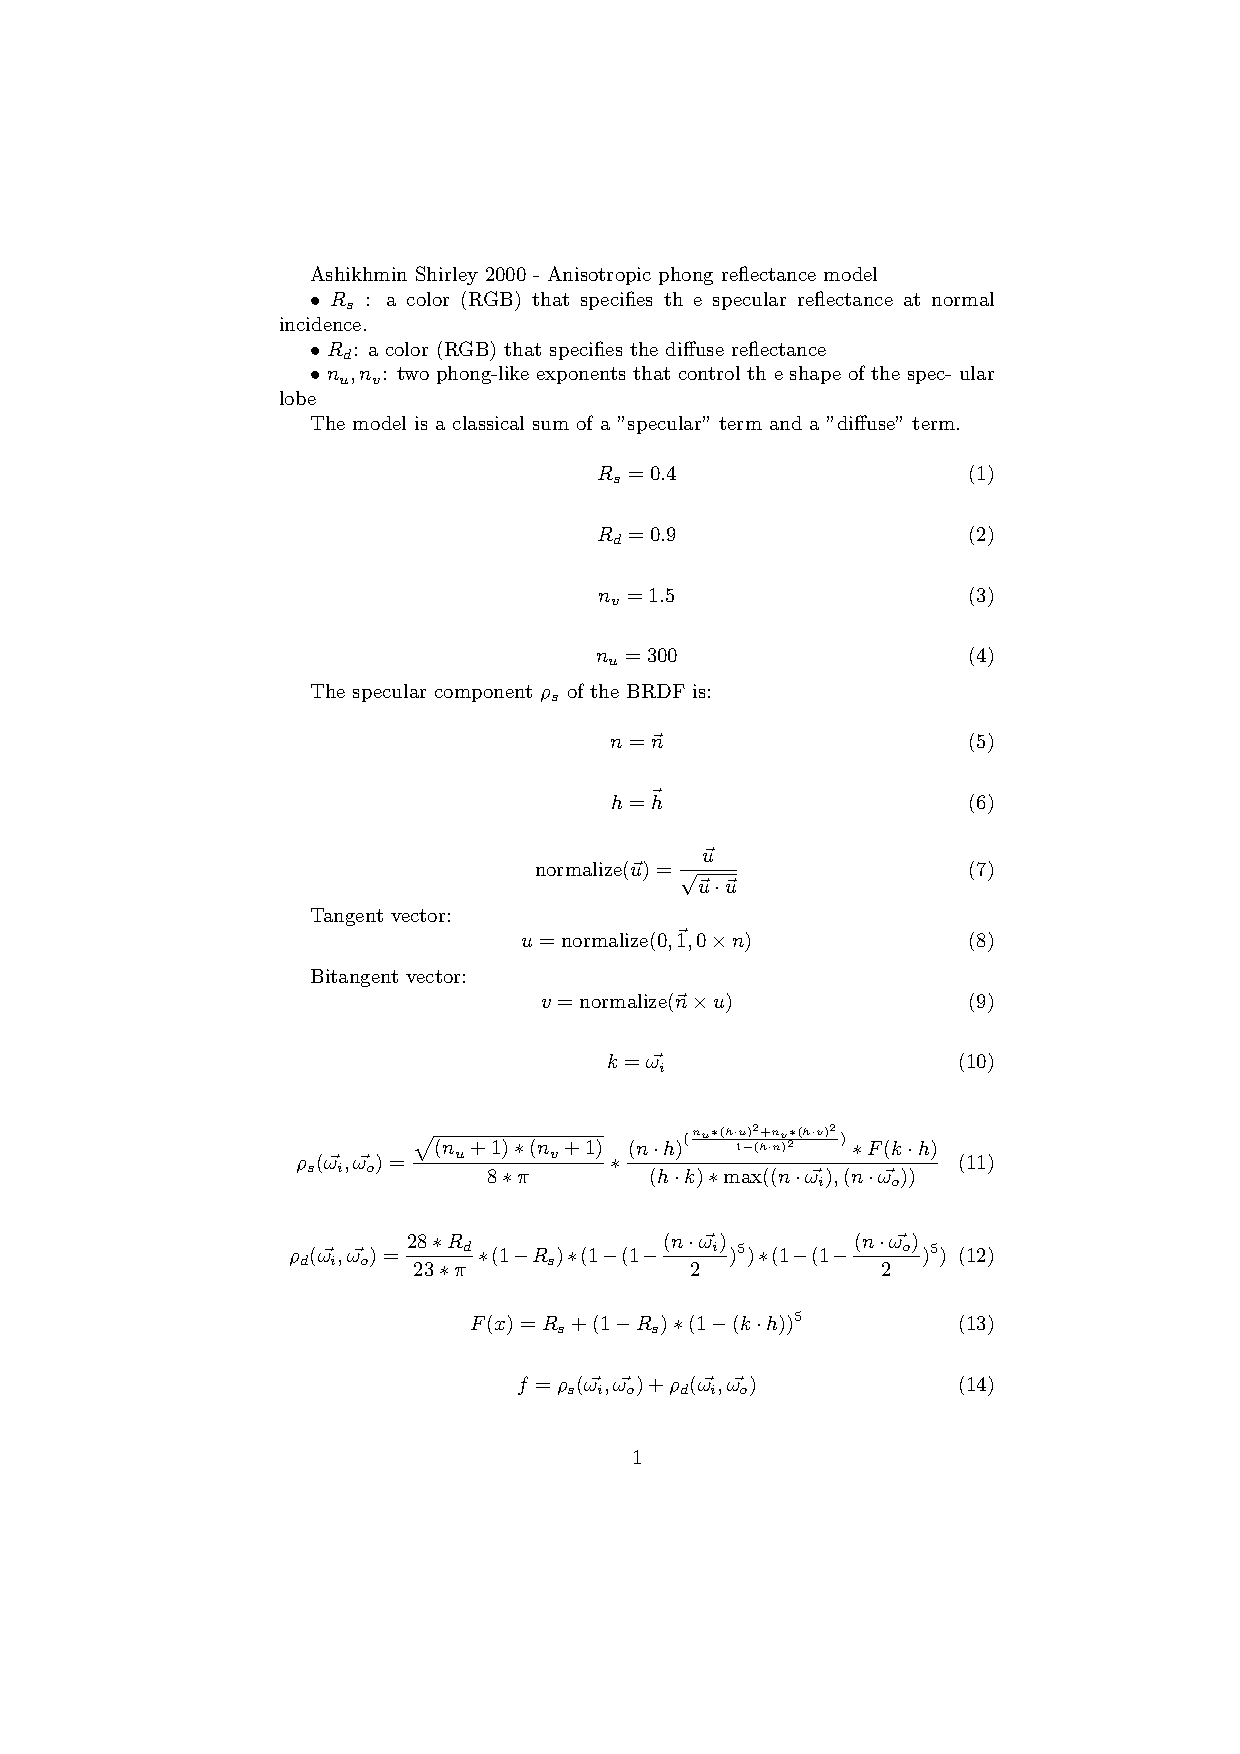
\includegraphics[scale=0.92]{./Imagens/brdfs/ashikhmin-shirley-close-to-original.pdf}
    \end{center}
\end{figure}


%%%%%%%%%%%%%%%%%%%%%%%%%%%%%%%%%%%%%%%%%%%%%%%%%
\subsection{Código Fonte em \texttt{EquationLang}}
%%%%%%%%%%%%%%%%%%%%%%%%%%%%%%%%%%%%%%%%%%%%%%%%%
\begin{codigo}[H]
    \caption{\small Código fonte da BRDF do experimento Ashikhmin-Shirley (parte 1 de 2).}
    \label{cod-ashikhmin-shirley-close-to-original-eqlang-pt-1}
\begin{lstlisting}[language=tex, frame=none, inputencoding=utf8]
Ashikhmin Shirley 2000 - Anisotropic phong reflectance model

 $R_s$ : a color (RGB) that specifies th e specular reflectance
at normal incidence.

 $R_d$: a color (RGB) that specifies the diffuse reflectance

 $n_u, n_v$: two phong-like exponents that control th e shape of the spec- ular lobe

The model is a classical sum of a "specular" term and a "diffuse" term.

\begin{equation}
    R_s = 0.4
\end{equation}

\begin{equation}
    R_d = 0.9
\end{equation}

\begin{equation}
    n_v = 1.5
\end{equation}

\begin{equation}
    n_u = 300
\end{equation}

The specular component $\rho_s$ of the BRDF is:

\begin{equation}
    n = \vec n
\end{equation}

\begin{equation}
    h = \vec h
\end{equation}
\end{equation}
\end{lstlisting}
\end{codigo}



\begin{codigo}[H]
    \caption{\small Código fonte da BRDF do experimento Ashikhmin-Shirley (parte 2 de 2).}
    \label{cod-ashikhmin-shirley-close-to-original-eqlang-pt-2}
\begin{lstlisting}[language=tex, frame=none, inputencoding=utf8]
\begin{equation}
  \text{normalize}(\vec{u}) = \frac{\vec{u}}{\sqrt{\vec{u} \cdot \vec{u}}}
\end{equation}
Tangent vector:
\begin{equation}
   u = \text{normalize}(\vec{0,1,0} \times n)
Bitangent vector:
\begin{equation}
   v = \text{normalize}(\vec{n} \times u)
\end{equation}

\begin{equation}
    k = \vec{\omega_i}
\end{equation}

\begin{equation}
    \rho_s(\vec{\omega_i}, \vec{\omega_o}) =
        \frac{\sqrt{(n_u+1)*(n_v+1)}}{8*\pi}
        * \frac{(n \cdot h)^{(\frac{n_u * (h \cdot u )^2 + n_v *(h \cdot v)^2}{1-(h \cdot n)^2})}
        * F(k \cdot h)}{(h \cdot k) * \max((n \cdot \vec{\omega_i}), (n \cdot \vec{\omega_o}) )}
\end{equation}

\begin{equation}
    \rho_d(\vec{\omega_i}, \vec{\omega_o}) = \frac{28*R_d}{23*\pi}
        * (1-R_s)
        * (1-(1-\frac{(n \cdot \vec{\omega_i})}{2})^5)
        * (1-(1-\frac{(n \cdot \vec{\omega_o})}{2})^5)
\end{equation}

\begin{equation}
    F(x) = R_s + (1-R_s)*(1-(k \cdot h))^5
\end{equation}

\begin{equation}
    f = \rho_s(\vec{\omega_i}, \vec{\omega_o}) + \rho_d(\vec{\omega_i}, \vec{\omega_o})
\end{equation}
\end{lstlisting}
\end{codigo}
%%%%%%%%%%%%%%%%%%%%%%%%%%%%%%%%%%%%%%%%%%%%%%%%%
\subsection{Código GLSL Gerado}
%%%%%%%%%%%%%%%%%%%%%%%%%%%%%%%%%%%%%%%%%%%%%%%%%
\begin{codigo}[H]
    \caption{\small Saída do compilador: código GLSL da BRDF do experimento Ashikhmin-Shirley (parte 1 de 2).}
    \label{cod-ashikhmin-shirley-close-to-original-glsl-pt-1}
\begin{lstlisting}[language=C, inputencoding=utf8]
analytic ::begin parameters
#[type][name][min val][max val][default val]
::end parameters
::begin shader
//////////// START OF BUILTINS DECLARTION ////////////
vec3 var_0_vec_h;
vec3 var_3_vec_n;
float var_10_theta_h;
float var_11_theta_d;
float var_1_pi;
float var_2_epsilon;
vec3 var_4_vec_omega_i;
float var_5_theta_i;
float var_6_phi_i;
vec3 var_7_vec_omega_o;
float var_8_theta_o;
float var_9_phi_o;
//////////// END OF BUILTINS DECLARTION ////////////
//////////// START OF USER DECLARED ////////////
vec3 var_12_k;
float var_13_n_v;
float var_14_n_u;
vec3 var_17_n;
vec3 var_18_u;
vec3 var_19_v;
float var_20_R_s;
vec3 var_21_h;
float var_24_R_d;
float var_27_f;
//////////// END OF USER DECLARED ////////////
//////////// START FUNCTIONS DECLARATIONS ////////////
vec3 var_15_text_normalize(vec3 var_16_vec_u) {
  return (var_16_vec_u / sqrt(dot(var_16_vec_u, var_16_vec_u)));
}
float var_22_F(float var_23_x) {
  return (var_20_R_s + (((1.0 - var_20_R_s)) *
                        pow(((1.0 - (dot(var_12_k, var_21_h)))), 5.0)));
}
float var_25_rho_d(vec3 var_4_vec_omega_i, vec3 var_7_vec_omega_o) {
  return (((((28.0 * var_24_R_d) / (23.0 * var_1_pi)) * ((1.0 - var_20_R_s))) *
       ((1.0 - pow(((1.0 - ((dot(var_17_n, var_4_vec_omega_i)) / 2.0))), 5.0)))) *
      ((1.0 - pow(((1.0 - ((dot(var_17_n, var_7_vec_omega_o)) / 2.0))), 5.0))));
}
\end{lstlisting}
\end{codigo}

\begin{codigo}[H]
    \caption{\small Saída do compilador: código GLSL da BRDF do experimento Ashikhmin-Shirley (parte 2 de 2).}
    \label{cod-ashikhmin-shirley-close-to-original-glsl-pt-2}
\begin{lstlisting}[language=C, inputencoding=utf8]
float var_26_rho_s(vec3 var_4_vec_omega_i, vec3 var_7_vec_omega_o) {
  return ((sqrt((((var_14_n_u + 1.0)) * ((var_13_n_v + 1.0)))) / (8.0 * var_1_pi)) *
      ((pow((dot(var_17_n, var_21_h)),
            ((((var_14_n_u * pow((dot(var_21_h, var_18_u)), 2.0)) +
            (var_13_n_v * pow((dot(var_21_h, var_19_v)), 2.0))) /
            (1.0 - pow((dot(var_21_h, var_17_n)), 2.0))))) *
        var_22_F(dot(var_12_k, var_21_h))) /
       ((dot(var_21_h, var_12_k)) * max((dot(var_17_n, var_4_vec_omega_i)),
                                        (dot(var_17_n, var_7_vec_omega_o))))));
}
//////////// END FUNCTIONS DECLARATIONS ////////////
vec3 BRDF(vec3 L, vec3 V, vec3 N, vec3 X, vec3 Y) {
  //////////// START OF BUILTINS INITIALIZATION ////////////
  var_0_vec_h = normalize(L + V);
  var_3_vec_n = normalize(N);
  var_1_pi = 3.141592653589793;
  var_2_epsilon = 1.192092896e-07;
  var_4_vec_omega_i = L;
  var_5_theta_i = atan(var_4_vec_omega_i.y, var_4_vec_omega_i.x);
  var_6_phi_i = atan(sqrt(var_4_vec_omega_i.y * var_4_vec_omega_i.y +
                          var_4_vec_omega_i.x * var_4_vec_omega_i.x),
                     var_4_vec_omega_i.z);
  var_7_vec_omega_o = V;
  var_8_theta_o = atan(var_7_vec_omega_o.y, var_7_vec_omega_o.x);
  var_9_phi_o = atan(sqrt(var_7_vec_omega_o.y * var_7_vec_omega_o.y +
                          var_7_vec_omega_o.x * var_7_vec_omega_o.x),
                     var_7_vec_omega_o.z);
  var_10_theta_h = acos(dot(var_0_vec_h, N));
  var_11_theta_d = acos(dot(var_0_vec_h, var_4_vec_omega_i));
  //////////// END OF BUILTINS INITIALIZATION ////////////
  var_12_k = var_4_vec_omega_i;
  var_13_n_v = 1.5;
  var_14_n_u = 300.0;
  var_17_n = var_3_vec_n;
  var_18_u = var_15_text_normalize(cross(vec3(0.0, 1.0, 0.0), var_17_n));
  var_19_v = var_15_text_normalize(cross(var_3_vec_n, var_18_u));
  var_20_R_s = 0.4;
  var_21_h = var_0_vec_h;
  var_24_R_d = 0.9;
  var_27_f = (var_26_rho_s(var_4_vec_omega_i, var_7_vec_omega_o) +
              var_25_rho_d(var_4_vec_omega_i, var_7_vec_omega_o));
  return vec3(var_27_f);
}
\end{lstlisting}
\end{codigo}

%%%%%%%%%%%%%%%%%%%%%%%%%%%%%%%%%%%%%%%%%%%%%%%%%
\subsection{Visualização do Resultado}
%%%%%%%%%%%%%%%%%%%%%%%%%%%%%%%%%%%%%%%%%%%%%%%%%

\begin{figure}[H]
    \caption{\small{\textit{Plots} da distribuição de reflexão especular e difusa do experimento Ashikhmin-Shirley.}}
    \label{fig-ashikhmin-shirley-close-to-original-plots}
\minipage{0.48\textwidth}
    \vspace{42px}
  
\includegraphics[width=\linewidth]{./Imagens/brdfs/ashikhmin-shirley-close-to-original-3D-plot}
    % \vspce{0.1px}
    \legend{ \small (a) 3D \textit{plot}}
\endminipage\hfill
\minipage{0.48\textwidth}
  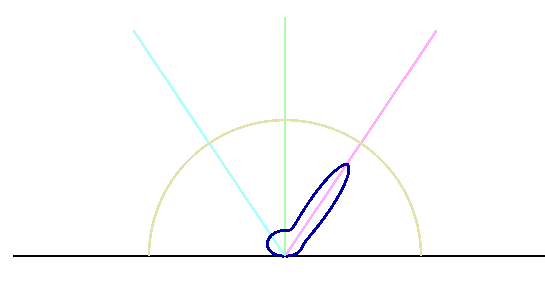
\includegraphics[width=\linewidth]{./Imagens/brdfs/ashikhmin-shirley-close-to-original-polar-plot.png}
    \legend{ \small (b) \textit{Polar plot}}
\endminipage\hfill
\end{figure}

\begin{figure}[H]
    \caption{\small{Objetos 3D renderizados pelo experimento Ashikhmin-Shirley.}}\label{fig-ashikhmin-shirley-close-to-original-eqlang}
\minipage{0.32\textwidth}
  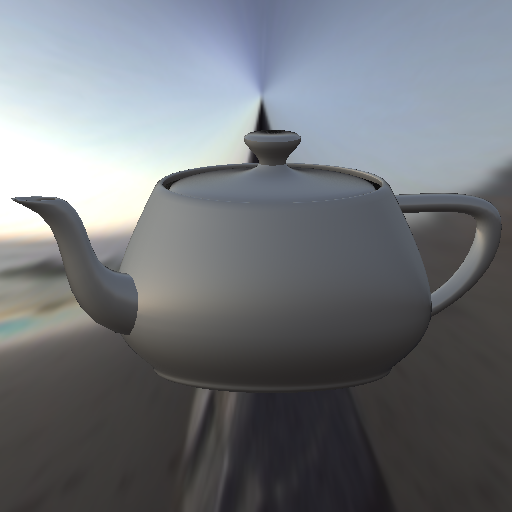
\includegraphics[width=\linewidth]{./Imagens/brdfs/ashikhmin-shirley-close-to-original-teapot.png}
    \legend{ \small (a) \textit{Teapot}}
\endminipage\hfill
\minipage{0.32\textwidth}
  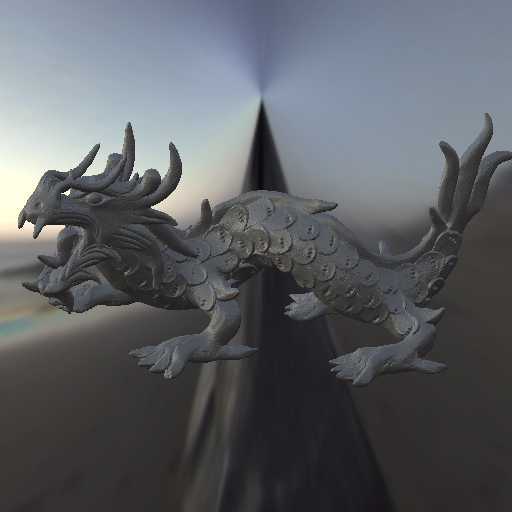
\includegraphics[width=\linewidth]{./Imagens/brdfs/ashikhmin-shirley-close-to-original-dragon.png}
    \legend{ \small (b) Dragão de Stanford}
\endminipage\hfill
\minipage{0.32\textwidth}%
  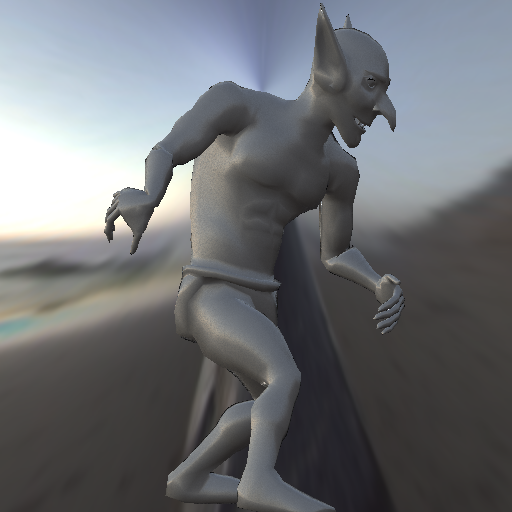
\includegraphics[width=\linewidth]{./Imagens/brdfs/ashikhmin-shirley-close-to-original-goblin.png}
    \legend{ \small (c) Goblin}
\endminipage
\end{figure}


\section{Experimento BRDF oren-nayar}

As equações que descrevem esse experimento se encontram em \autoref{fig-oren-nayar-eqlang-latex}. O código fonte de entrada para o compilador está dividido em duas partes, parte 1 está no \autoref{cod-oren-nayar-eqlang} e a segunda parte está em \autoref{cod-oren-nayar-eqlang-pt2}. A renderização dos objetos 3D usando essa BRDF se encontra em \autoref{fig-oren-nayar-eqlang}.

%%%%%%%%%%%%%%%%%%%%%%%%%%%%%%%%%%%%%%%%%%%%%%%%%
\subsection{Representação em documento \LaTeX{}}
%%%%%%%%%%%%%%%%%%%%%%%%%%%%%%%%%%%%%%%%%%%%%%%%%
\begin{figure}[H]
    \caption{\label{fig-oren-nayar-eqlang-latex} \small Equações da BRDF do experimento oren-nayar em documento \LaTeX{}.}
    \begin{center}
        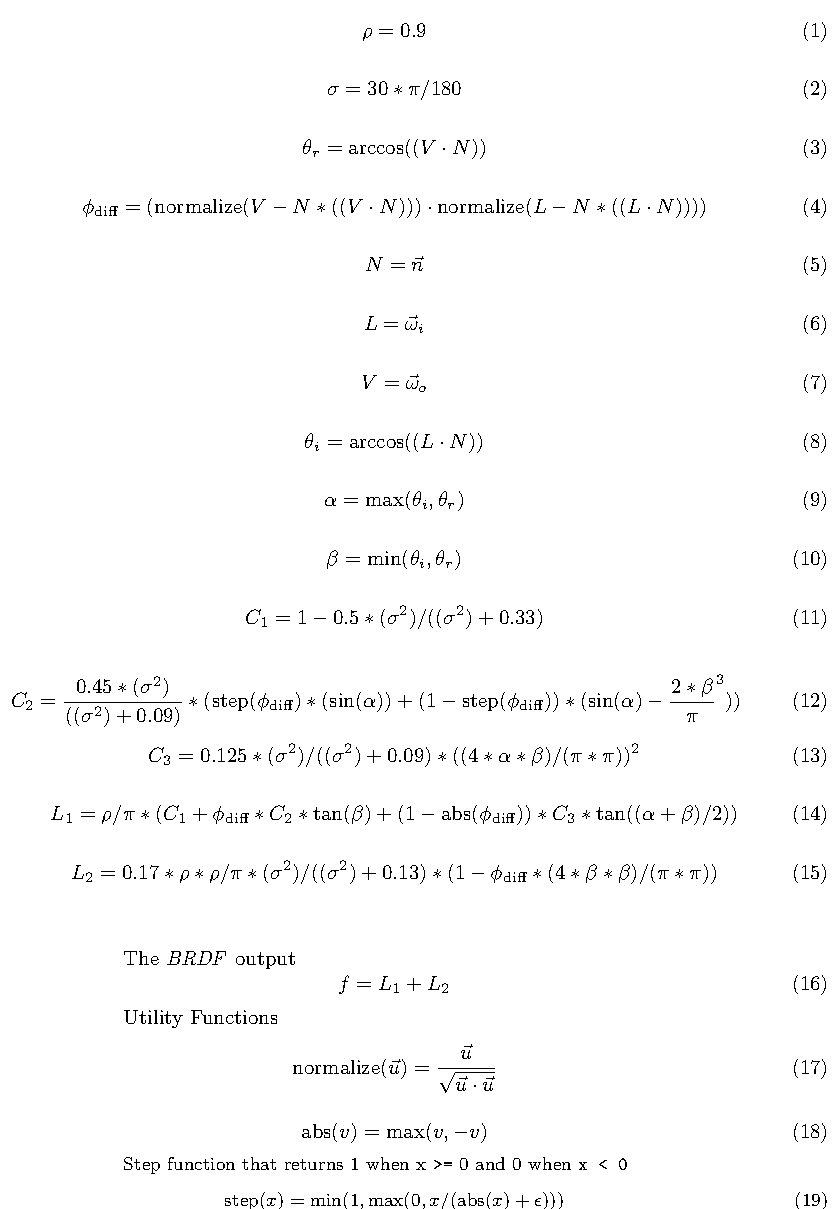
\includegraphics[scale=0.82]{./Imagens/brdfs/oren-nayar.pdf}
    \end{center}
\end{figure}

%%%%%%%%%%%%%%%%%%%%%%%%%%%%%%%%%%%%%%%%%%%%%%%%%
\subsection{Visualização do Resultado}
%%%%%%%%%%%%%%%%%%%%%%%%%%%%%%%%%%%%%%%%%%%%%%%%%
\begin{figure}[H]
    \caption{\small{Distribuição de Reflexão Especular e Difusa da BRDF}}\label{fig-oren-nayar-eqlang}
\minipage{0.48\textwidth}
    \vspace{42px}
  
\includegraphics[width=\linewidth]{./Imagens/brdfs/oren-nayar-3D-plot}
    % \vspace{0.1px}
    \legend{ \small (a) 3D \textit{plot}}
\endminipage\hfill
\minipage{0.48\textwidth}
  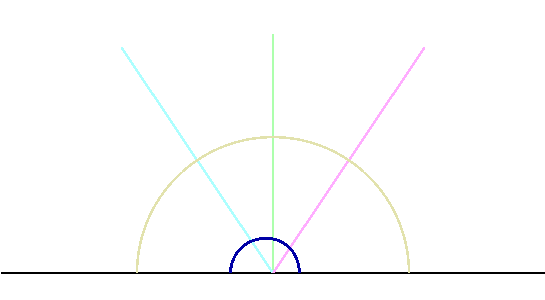
\includegraphics[width=\linewidth]{./Imagens/brdfs/oren-nayar-polar-plot.png}
    \legend{ \small (b) \textit{Polar plot}}
\endminipage\hfill
\end{figure}

\begin{figure}[H]
    \caption{\small{Objetos 3D renderizados por este experimento}}\label{fig-oren-nayar-eqlang}
\minipage{0.32\textwidth}
  \includegraphics[width=\linewidth]{./Imagens/brdfs/oren-nayar-teapot.png}
    \legend{ \small (a) \textit{Teapot}}
\endminipage\hfill
\minipage{0.32\textwidth}
  \includegraphics[width=\linewidth]{./Imagens/brdfs/oren-nayar-dragon.png}
    \legend{ \small (b) Dragão de Stanford}
\endminipage\hfill
\minipage{0.32\textwidth}%
  \includegraphics[width=\linewidth]{./Imagens/brdfs/oren-nayar-goblin.png}
    \legend{ \small (c) Goblin}
\endminipage
\end{figure}

%%%%%%%%%%%%%%%%%%%%%%%%%%%%%%%%%%%%%%%%%%%%%%%%%
\subsection{Código GLSL Gerado}
%%%%%%%%%%%%%%%%%%%%%%%%%%%%%%%%%%%%%%%%%%%%%%%%%
\begin{codigo}[H]
    \caption{\small Saida do compilador, código GLSL da BRDF deste experimento (parte 1). }
    \label{cod-oren-nayar-eqlang-declarations}
\begin{lstlisting}[language=C, inputencoding=utf8]
\end{lstlisting}
\end{codigo}

\begin{codigo}[H]
    \caption{\small Saida do compilador, código GLSL da BRDF deste experimento  (parte 2). }
    \label{cod-oren-nayar-eqlang}
\begin{lstlisting}[language=C, inputencoding=utf8]
\end{lstlisting}
\end{codigo}

%%%%%%%%%%%%%%%%%%%%%%%%%%%%%%%%%%%%%%%%%%%%%%%%%
\subsection{Código Fonte em \texttt{EquationLang}}
%%%%%%%%%%%%%%%%%%%%%%%%%%%%%%%%%%%%%%%%%%%%%%%%%
\begin{codigo}[H]
    \caption{\small Código fonte da BRDF deste experimento (parte 1).}
    \label{cod-oren-nayar-eqlang}
\begin{lstlisting}[language=tex, frame=none, inputencoding=utf8]
\end{lstlisting}
\end{codigo}

\section{Experimento BRDF Ashikhmin-Shirley Alternativa}


Nesse caso, foi realizado uma versão alternativa do experimento da \autoref{sec:ashikhmin-shirley}. As equações na \autoref{fig-ashikhmin-shirley-alternative-eqlang-latex} estão simplicadas e algumas equações foram comprimidas em uma só. Além disso, nessa versão, foram escolhidas diferentes constantes, como cor difusa, fatores de multiplicação, entre outros. Código fonte em \texttt{EquationLang} disponível no \autoref{cod-ashikhmin-shirley-alternative-eqlang}. Os códigos gerados em GLSL estão no \autoref{cod-ashikhmin-shirley-alternative-glsl-pt-1} e \autoref{cod-ashikhmin-shirley-alternative-glsl-pt-2}. Objetos 3D renderizados pode ser vistos na \autoref{fig-ashikhmin-shirley-alternative-eqlang} e os plots estão na \autoref{fig-ashikhmin-shirley-alternative-plots}.
%%%%%%%%%%%%%%%%%%%%%%%%%%%%%%%%%%%%%%%%%%%%%%%%%
\subsection{Representação em documento \LaTeX{}}
%%%%%%%%%%%%%%%%%%%%%%%%%%%%%%%%%%%%%%%%%%%%%%%%%
\begin{figure}[H]
    \caption{\label{fig-ashikhmin-shirley-alternative-eqlang-latex} \small Equações da BRDF do experimento ashikhmin-shirley-alternative em documento \LaTeX{}.}
    \begin{center}
        \includegraphics[scale=0.92]{./Imagens/brdfs/ashikhmin-shirley-alternative.pdf}
    \end{center}
\end{figure}

%%%%%%%%%%%%%%%%%%%%%%%%%%%%%%%%%%%%%%%%%%%%%%%%%
\subsection{Visualização do Resultado}
%%%%%%%%%%%%%%%%%%%%%%%%%%%%%%%%%%%%%%%%%%%%%%%%%
\begin{figure}[H]
    \caption{\small{Distribuição de Reflexão Especular e Difusa da BRDF}}\label{fig-ashikhmin-shirley-alternative-plots}
\minipage{0.48\textwidth}
    \vspace{42px}
  \includegraphics[width=\linewidth]{./Imagens/brdfs/ashikhmin-shirley-alternative-3D-plot}
    % \vspace{0.1px}
    \legend{ \small (a) 3D \textit{plot}}
\endminipage\hfill
\minipage{0.48\textwidth}
  \includegraphics[width=\linewidth]{./Imagens/brdfs/ashikhmin-shirley-alternative-polar-plot.png}
    \legend{ \small (b) \textit{Polar plot}}
\endminipage\hfill
\end{figure}

\begin{figure}[H]
    \caption{\small{Objetos 3D renderizados por este experimento}}\label{fig-ashikhmin-shirley-alternative-eqlang}
\minipage{0.32\textwidth}
  \includegraphics[width=\linewidth]{./Imagens/brdfs/ashikhmin-shirley-alternative-teapot.png}
    \legend{ \small (a) \textit{Teapot}}
\endminipage\hfill
\minipage{0.32\textwidth}
  \includegraphics[width=\linewidth]{./Imagens/brdfs/ashikhmin-shirley-alternative-dragon.png}
    \legend{ \small (b) Dragão de Stanford}
\endminipage\hfill
\minipage{0.32\textwidth}%
  \includegraphics[width=\linewidth]{./Imagens/brdfs/ashikhmin-shirley-alternative-goblin.png}
    \legend{ \small (c) Goblin}
\endminipage
\end{figure}

%%%%%%%%%%%%%%%%%%%%%%%%%%%%%%%%%%%%%%%%%%%%%%%%%
\subsection{Código GLSL Gerado}
%%%%%%%%%%%%%%%%%%%%%%%%%%%%%%%%%%%%%%%%%%%%%%%%%
\begin{codigo}[H]
    \caption{\small Saida do compilador, código GLSL da BRDF deste experimento (parte 1). }
    \label{cod-ashikhmin-shirley-alternative-glsl-pt-1}
\begin{lstlisting}[language=C, inputencoding=utf8]
analytic ::begin parameters
#[type][name][min val][max val][default val]
::end parameters
::begin shader
//////////// START OF BUILTINS DECLARTION ////////////
vec3 var_0_vec_h;
vec3 var_3_vec_n;
float var_10_theta_h;
float var_11_theta_d;
float var_1_pi;
float var_2_epsilon;
vec3 var_4_vec_omega_i;
float var_5_theta_i;
float var_6_phi_i;
vec3 var_7_vec_omega_o;
float var_8_theta_o;
float var_9_phi_o;
//////////// END OF BUILTINS DECLARTION ////////////

//////////// START OF USER DECLARED ////////////
vec3 var_12_rho_d;
vec3 var_13_rho_s;
vec3 var_14_f;
//////////// END OF USER DECLARED ////////////
\end{lstlisting}
\end{codigo}

\begin{codigo}[H]
    \caption{\small Saida do compilador, código GLSL da BRDF deste experimento  (parte 2). }
    \label{cod-ashikhmin-shirley-alternative-glsl-pt-2}
\begin{lstlisting}[language=C, inputencoding=utf8]
//////////// START FUNCTIONS DECLARATIONS ////////////
//////////// END FUNCTIONS DECLARATIONS ////////////

vec3 BRDF(vec3 L, vec3 V, vec3 N, vec3 X, vec3 Y) {

  //////////// START OF BUILTINS INITIALIZATION ////////////
  var_0_vec_h = normalize(L + V);
  var_3_vec_n = normalize(N);
  var_1_pi = 3.141592653589793;
  var_2_epsilon = 1.192092896e-07;
  var_4_vec_omega_i = L;
  var_5_theta_i = atan(var_4_vec_omega_i.y, var_4_vec_omega_i.x);
  var_6_phi_i = atan(sqrt(var_4_vec_omega_i.y * var_4_vec_omega_i.y +
                          var_4_vec_omega_i.x * var_4_vec_omega_i.x),
                     var_4_vec_omega_i.z);
  var_7_vec_omega_o = V;
  var_8_theta_o = atan(var_7_vec_omega_o.y, var_7_vec_omega_o.x);
  var_9_phi_o = atan(sqrt(var_7_vec_omega_o.y * var_7_vec_omega_o.y +
                          var_7_vec_omega_o.x * var_7_vec_omega_o.x),
                     var_7_vec_omega_o.z);
  var_10_theta_h = acos(dot(var_0_vec_h, N));
  var_11_theta_d = acos(dot(var_0_vec_h, var_4_vec_omega_i));
  //////////// END OF BUILTINS INITIALIZATION ////////////

  var_12_rho_d = vec3(0.3, 0.3, 0.3);
  var_13_rho_s = (vec3(0.0, 0.2, 1.0) * 20.0);
  var_14_f = ((var_12_rho_d / var_1_pi) +
              ((var_13_rho_s / (8.0 * var_1_pi)) *
               ((dot(var_3_vec_n, var_0_vec_h)) /
                ((dot(var_7_vec_omega_o, var_0_vec_h)) *
                 max((dot(var_3_vec_n, var_4_vec_omega_i)),
                     (dot(var_3_vec_n, var_7_vec_omega_o)))))));

  return vec3(var_14_f);
}
\end{lstlisting}
\end{codigo}

%%%%%%%%%%%%%%%%%%%%%%%%%%%%%%%%%%%%%%%%%%%%%%%%%
\subsection{Código Fonte em \texttt{EquationLang}}
%%%%%%%%%%%%%%%%%%%%%%%%%%%%%%%%%%%%%%%%%%%%%%%%%
\begin{codigo}[H]
    \caption{\small Código fonte da BRDF deste experimento.}
    \label{cod-ashikhmin-shirley-alternative-eqlang}
\begin{lstlisting}[language=tex, frame=none, inputencoding=utf8]

\begin{document}

\begin{equation}
    \rho_{d} = \vec{0.3,0.3,0.3}
\end{equation}

\begin{equation}
    \rho_{s} = \vec{0.0,0.2,1.0}*20
\end{equation}

\begin{equation}
f = \frac{\rho_{d}}{\pi} + \frac{\rho_{s}}{8*\pi} *
\frac{({\vec{n}}\cdot{\vec{h}})}
{({\vec{\omega_{o}}}\cdot{\vec{h}}) *
\max(({\vec{n}}\cdot{\vec{\omega_{i}}}),
({\vec{n}}\cdot{\vec{\omega_{o}}}))}
\end{equation}

\end{lstlisting}
\end{codigo}


\section{Experimento BRDF Cook-Torrance Alternativa}
\label{section-experiment-cook-torrance-alternative}

Este experimento é uma versão alternativa da realizada na \autoref{sec:cook-torrance}. As equações apresentadas na \autoref{fig-cook-torrance-alternative-eqlang-latex} incorporam a equação do efeito Fresnel e utilizam constantes distintas. O código-fonte em \texttt{EquationLang} pode ser consultado no \autoref{cod-cook-torrance-alternative-eqlang}. O código gerado em GLSL está no \autoref{cod-cook-torrance-alternative-glsl-pt-1} e no \autoref{cod-cook-torrance-alternative-glsl-pt-2}. Objetos 3D renderizados podem ser vistos na \autoref{fig-cook-torrance-alternative-eqlang} e os \textit{plots} estão na \autoref{fig-cook-torrance-alternative-plots}.


%%%%%%%%%%%%%%%%%%%%%%%%%%%%%%%%%%%%%%%%%%%%%%%%%
\subsection{Representação em documento \LaTeX{}}
%%%%%%%%%%%%%%%%%%%%%%%%%%%%%%%%%%%%%%%%%%%%%%%%%
\begin{figure}[H]
    \caption{\label{fig-cook-torrance-alternative-eqlang-latex}
    \small Equações da BRDF do experimento Cook-Torrance$_2$ (alternativa) em documento \LaTeX{}.}
    \begin{center}
        \includegraphics[scale=0.92]{./Imagens/brdfs/cook-torrance-alternative.pdf}
    \end{center}
\end{figure}

%%%%%%%%%%%%%%%%%%%%%%%%%%%%%%%%%%%%%%%%%%%%%%%%%
\subsection{Código Fonte em \texttt{EquationLang}}
%%%%%%%%%%%%%%%%%%%%%%%%%%%%%%%%%%%%%%%%%%%%%%%%%
\begin{codigo}[H]
    \caption{\small Código fonte da BRDF do experimento Cook-Torrance$_2$.}
    \label{cod-cook-torrance-alternative-eqlang}
\begin{lstlisting}[language=tex, frame=none, inputencoding=utf8]
\begin{equation}
    m = 0.3
\end{equation}
\begin{equation}
    f_0 = 0.4
\end{equation}
\begin{equation}
Beckmann(m, t) = \exp((t*t-1)/(m*m*t*t)) / (m*m*t*t*t*t)
\end{equation}
\begin{equation}
    Fresnel(f_0, u) = f_0 + (1 - f_0) * ((1-u)^ 5)
\end{equation}
\begin{equation}
    H = \vec{h}
\end{equation}
\begin{equation}
    V = \vec{\omega_o}
\end{equation}
\begin{equation}
    L = \vec{\omega_{i}}
\end{equation}
\begin{equation}
    N = \vec{n}
\end{equation}
\begin{equation}
    D = Beckmann(m,  (N \cdot H) )
\end{equation}
\begin{equation}
    F = Fresnel(f_0,  (V \cdot H) )
\end{equation}
\begin{equation}
G = 1/(N \cdot V)
\end{equation}
\begin{equation}
    val = \max(D * G, 0.0) \cdot F
\end{equation}
\begin{equation}
    \text{color} = \vec{1,0.5,1}
\end{equation}
\begin{equation}
    f = \text{color} * val / (N \cdot L)
\end{equation}
\end{lstlisting}
\end{codigo}

%%%%%%%%%%%%%%%%%%%%%%%%%%%%%%%%%%%%%%%%%%%%%%%%%
\subsection{Código GLSL Gerado}
%%%%%%%%%%%%%%%%%%%%%%%%%%%%%%%%%%%%%%%%%%%%%%%%%
\begin{codigo}[H]
    \caption{\small Saída do compilador: código GLSL da BRDF do experimento Cook-Torrance$_2$ (parte 1 de 2).}
    \label{cod-cook-torrance-alternative-glsl-pt-1}
\begin{lstlisting}[language=C, inputencoding=utf8]
analytic ::begin parameters
#[type][name][min val][max val][default val]
::end parameters
::begin shader
//////////// START OF BUILTINS DECLARTION ////////////
vec3 var_0_vec_h;
vec3 var_3_vec_n;
float var_10_theta_h;
float var_11_theta_d;
float var_1_pi;
float var_2_epsilon;
vec3 var_4_vec_omega_i;
float var_5_theta_i;
float var_6_phi_i;
vec3 var_7_vec_omega_o;
float var_8_theta_o;
float var_9_phi_o;
//////////// END OF BUILTINS DECLARTION ////////////
//////////// START OF USER DECLARED ////////////
vec3 var_12_V;
vec3 var_13_L;
float var_17_f_0;
float var_15_m;
vec3 var_20_H;
vec3 var_21_text_color;
vec3 var_22_N;
float var_23_D;
float var_24_G;
float var_25_F;
float var_26_val;
vec3 var_27_f;
\end{lstlisting}
\end{codigo}

\begin{codigo}[H]
    \caption{\small Saída do compilador: código GLSL da BRDF do experimento Cook-Torrance$_2$ (parte 2 de 2).}
    \label{cod-cook-torrance-alternative-glsl-pt-2}
\begin{lstlisting}[language=C, inputencoding=utf8]
//////////// END OF USER DECLARED ////////////
//////////// START FUNCTIONS DECLARATIONS ////////////
float var_14_Beckmann(float var_15_m, float var_16_t) {
  return (exp((((((var_16_t * var_16_t) - 1.0)) /
                ((((var_15_m * var_15_m) * var_16_t) * var_16_t))))) /
          ((((((var_15_m * var_15_m) * var_16_t) * var_16_t) * var_16_t) *
            var_16_t)));
}
float var_18_Fresnel(float var_17_f_0, float var_19_u) {
  return (var_17_f_0 + (((1.0 - var_17_f_0)) * (pow(((1.0 - var_19_u)), 5.0))));
}
//////////// END FUNCTIONS DECLARATIONS ////////////
//////////// END FUNCTIONS DECLARATIONS ////////////
vec3 BRDF(vec3 L, vec3 V, vec3 N, vec3 X, vec3 Y) {
  //////////// START OF BUILTINS INITIALIZATION ////////////
  var_0_vec_h = normalize(L + V);
  var_3_vec_n = normalize(N);
  var_1_pi = 3.141592653589793;
  var_2_epsilon = 1.192092896e-07;
  var_4_vec_omega_i = L;
  var_5_theta_i = atan(var_4_vec_omega_i.y, var_4_vec_omega_i.x);
  var_6_phi_i = atan(sqrt(var_4_vec_omega_i.y * var_4_vec_omega_i.y +
                          var_4_vec_omega_i.x * var_4_vec_omega_i.x),
                     var_4_vec_omega_i.z);
  var_7_vec_omega_o = V;
  var_8_theta_o = atan(var_7_vec_omega_o.y, var_7_vec_omega_o.x);
  var_9_phi_o = atan(sqrt(var_7_vec_omega_o.y * var_7_vec_omega_o.y +
                          var_7_vec_omega_o.x * var_7_vec_omega_o.x),
                     var_7_vec_omega_o.z);
  var_10_theta_h = acos(dot(var_0_vec_h, N));
  var_11_theta_d = acos(dot(var_0_vec_h, var_4_vec_omega_i));
  //////////// END OF BUILTINS INITIALIZATION ////////////

  var_12_V = var_7_vec_omega_o;
  var_13_L = var_4_vec_omega_i;
  var_17_f_0 = 0.4;
  var_15_m = 0.3;
  var_20_H = var_0_vec_h;
  var_21_text_color = vec3(1.0, 0.5, 1.0);
  var_22_N = var_3_vec_n;
  var_23_D = var_14_Beckmann(var_15_m, (dot(var_22_N, var_20_H)));
  var_24_G = (1.0 / (dot(var_22_N, var_12_V)));
  var_25_F = var_18_Fresnel(var_17_f_0, (dot(var_12_V, var_20_H)));
  var_26_val = (max((var_23_D * var_24_G), 0.0) * var_25_F);
  var_27_f = ((var_21_text_color * var_26_val) / (dot(var_22_N, var_13_L)));

  return vec3(var_27_f);
}
\end{lstlisting}
\end{codigo}

%%%%%%%%%%%%%%%%%%%%%%%%%%%%%%%%%%%%%%%%%%%%%%%%%
\subsection{Visualização do Resultado}
%%%%%%%%%%%%%%%%%%%%%%%%%%%%%%%%%%%%%%%%%%%%%%%%%
\begin{figure}[H]
    \caption{\small{\textit{Plots} da distribuição de reflexão especular e difusa do experimento Cook-Torrance$_2$.}}
    \label{fig-cook-torrance-alternative-plots}
\minipage{0.48\textwidth}
    \vspace{42px}
  \includegraphics[width=\linewidth]{./Imagens/brdfs/cook-torrance-alternative-3D-plot}
    % \vspace{0.1px}
    \legend{ \small (a) 3D \textit{plot}}
\endminipage\hfill
\minipage{0.48\textwidth}
  \includegraphics[width=\linewidth]{./Imagens/brdfs/cook-torrance-alternative-polar-plot-log.png}
    \legend{ \small (b) \textit{Polar plot}}
\endminipage\hfill
\end{figure}

\begin{figure}[H]
    \caption{\small{Objetos 3D renderizados pelo experimento Cook-Torrance$_2$.}}\label{fig-cook-torrance-alternative-eqlang}
\minipage{0.32\textwidth}
  \includegraphics[width=\linewidth]{./Imagens/brdfs/cook-torrance-alternative-teapot.png}
    \legend{ \small (a) \textit{Teapot}}
\endminipage\hfill
\minipage{0.32\textwidth}
  \includegraphics[width=\linewidth]{./Imagens/brdfs/cook-torrance-alternative-dragon.png}
    \legend{ \small (b) Dragão de Stanford}
\endminipage\hfill
\minipage{0.32\textwidth}%
  \includegraphics[width=\linewidth]{./Imagens/brdfs/cook-torrance-alternative-goblin.png}
    \legend{ \small (c) Goblin}
\endminipage
\end{figure}


\section{Experimento BRDF Dür}
\label{section-experiment-duer}

No artigo de Geisler-Moroder e Dür \cite{duer2010bounding}, são discutidas as limitações do modelo de reflexão de Ward, propondo uma abordagem para restringir o albedo e garantir a conservação de energia. Este experimento é baseado nessa BRDF com albedo restringido. As equações são apresentadas na \autoref{fig-duer-eqlang-latex}, com o código fonte em \texttt{EquationLang} disponível no \autoref{cod-duer-eqlang}. Os códigos gerados em GLSL podem ser vistos no \autoref{cod-duer-glsl-pt-1} e no \autoref{cod-duer-glsl-pt-2}. A renderização dos objetos 3D pode ser observada na \autoref{fig-duer-eqlang} e os \textit{plots} na \autoref{fig-duer-plots}.

%%%%%%%%%%%%%%%%%%%%%%%%%%%%%%%%%%%%%%%%%%%%%%%%%
\subsection{Representação em documento \LaTeX{}}
%%%%%%%%%%%%%%%%%%%%%%%%%%%%%%%%%%%%%%%%%%%%%%%%%
\begin{figure}[H]
    \caption{\label{fig-duer-eqlang-latex} \small Equações da BRDF do experimento Dür em documento \LaTeX{}.}
    \begin{center}
        \includegraphics[scale=0.92]{./Imagens/brdfs/duer.pdf}
    \end{center}
\end{figure}

%%%%%%%%%%%%%%%%%%%%%%%%%%%%%%%%%%%%%%%%%%%%%%%%%
\subsection{Código Fonte em \texttt{EquationLang}}
%%%%%%%%%%%%%%%%%%%%%%%%%%%%%%%%%%%%%%%%%%%%%%%%%
\begin{codigo}[H]
    \caption{\small Código fonte da BRDF do experimento Dür.}
    \label{cod-duer-eqlang}
\begin{lstlisting}[language=tex, frame=none, inputencoding=utf8]
Duer 2010 Bounding the Albedo of the Ward Reflectance Model

\begin{equation}
G = ((\vec{\omega_i}+\vec{\omega_o}) \cdot(\vec{\omega_i}+\vec{\omega_o})) * ((\vec{\omega_i}+\vec{\omega_o}) \cdot \vec{n})^-4
    * (\vec{n} \cdot \vec{\omega_i})*(\vec{n} \cdot \vec{\omega_o})
\end{equation}

\begin{equation}
f =  G
\end{equation}
\end{lstlisting}
\end{codigo}

%%%%%%%%%%%%%%%%%%%%%%%%%%%%%%%%%%%%%%%%%%%%%%%%%
\subsection{Código GLSL Gerado}
%%%%%%%%%%%%%%%%%%%%%%%%%%%%%%%%%%%%%%%%%%%%%%%%%
\begin{codigo}[H]
    \caption{\small Saída do compilador: código GLSL da BRDF do experimento Dür (parte 1 de 2).}
    \label{cod-duer-glsl-pt-1}
\begin{lstlisting}[language=C, inputencoding=utf8]
analytic ::begin parameters
#[type][name][min val][max val][default val]
::end parameters
::begin shader
//////////// START OF BUILTINS DECLARTION ////////////
vec3 var_0_vec_h;
vec3 var_3_vec_n;
float var_10_theta_h;
float var_11_theta_d;
float var_1_pi;
float var_2_epsilon;
vec3 var_4_vec_omega_i;
float var_5_theta_i;
float var_6_phi_i;
vec3 var_7_vec_omega_o;
float var_8_theta_o;
float var_9_phi_o;
//////////// END OF BUILTINS DECLARTION ////////////
//////////// START OF USER DECLARED ////////////
float var_12_G;
float var_13_f;
//////////// END OF USER DECLARED ////////////
//////////// START FUNCTIONS DECLARATIONS ////////////
//////////// END FUNCTIONS DECLARATIONS ////////////

\end{lstlisting}
\end{codigo}

\begin{codigo}[H]
    \caption{\small Saída do compilador: código GLSL da BRDF do experimento Dür (parte 2 de 2).}
    \label{cod-duer-glsl-pt-2}
\begin{lstlisting}[language=C, inputencoding=utf8]
vec3 BRDF(vec3 L, vec3 V, vec3 N, vec3 X, vec3 Y) {

  //////////// START OF BUILTINS INITIALIZATION ////////////
  var_0_vec_h = normalize(L + V);
  var_3_vec_n = normalize(N);
  var_1_pi = 3.141592653589793;
  var_2_epsilon = 1.192092896e-07;
  var_4_vec_omega_i = L;
  var_5_theta_i = atan(var_4_vec_omega_i.y, var_4_vec_omega_i.x);
  var_6_phi_i = atan(sqrt(var_4_vec_omega_i.y * var_4_vec_omega_i.y +
                          var_4_vec_omega_i.x * var_4_vec_omega_i.x),
                     var_4_vec_omega_i.z);
  var_7_vec_omega_o = V;
  var_8_theta_o = atan(var_7_vec_omega_o.y, var_7_vec_omega_o.x);
  var_9_phi_o = atan(sqrt(var_7_vec_omega_o.y * var_7_vec_omega_o.y +
                          var_7_vec_omega_o.x * var_7_vec_omega_o.x),
                     var_7_vec_omega_o.z);
  var_10_theta_h = acos(dot(var_0_vec_h, N));
  var_11_theta_d = acos(dot(var_0_vec_h, var_4_vec_omega_i));
  //////////// END OF BUILTINS INITIALIZATION ////////////

  var_12_G =
      ((((dot(((var_4_vec_omega_i + var_7_vec_omega_o)),
              ((var_4_vec_omega_i + var_7_vec_omega_o)))) *
         pow((dot(((var_4_vec_omega_i + var_7_vec_omega_o)), var_3_vec_n)),
             (-4.0))) *
        (dot(var_3_vec_n, var_4_vec_omega_i))) *
       (dot(var_3_vec_n, var_7_vec_omega_o)));
  var_13_f = var_12_G;

  return vec3(var_13_f);
}
\end{lstlisting}
\end{codigo}


%%%%%%%%%%%%%%%%%%%%%%%%%%%%%%%%%%%%%%%%%%%%%%%%%
\subsection{Visualização do Resultado}
%%%%%%%%%%%%%%%%%%%%%%%%%%%%%%%%%%%%%%%%%%%%%%%%%
\begin{figure}[H]
    \caption{\small{\textit{Plots} da distribuição de reflexão especular e difusa do experimento Dür.}}
    \label{fig-duer-plots}
\minipage{0.48\textwidth}
    \vspace{42px}
  \includegraphics[width=\linewidth]{./Imagens/brdfs/duer-3D-plot}
    % \vspace{0.1px}
    \legend{ \small (a) 3D \textit{plot}}
\endminipage\hfill
\minipage{0.48\textwidth}
  \includegraphics[width=\linewidth]{./Imagens/brdfs/duer-polar-plot.png}
    \legend{ \small (b) \textit{Polar plot}}
\endminipage\hfill
\end{figure}

\begin{figure}[H]
    \caption{\small{Objetos 3D renderizados pelo experimento Dür.}}
    \label{fig-duer-eqlang}
\minipage{0.32\textwidth}
  \includegraphics[width=\linewidth]{./Imagens/brdfs/duer-teapot.png}
    \legend{ \small (a) \textit{Teapot}}
\endminipage\hfill
\minipage{0.32\textwidth}
  \includegraphics[width=\linewidth]{./Imagens/brdfs/duer-dragon.png}
    \legend{ \small (b) Dragão de Stanford}
\endminipage\hfill
\minipage{0.32\textwidth}%
  \includegraphics[width=\linewidth]{./Imagens/brdfs/duer-goblin.png}
    \legend{ \small (c) Goblin}
\endminipage
\end{figure}



\section{Experimento BRDF Edwards 2006}
\label{section-experiment-edwards-2006}

No artigo de Edwards et al. \cite{edwards2006halfway}, é apresentado o conceito do \textit{Halfway Vector Disk} como uma extensão para modelagem de BRDFs. Este método, usado neste experimento, propõe uma ideia geométrica que melhora a eficiência computacional. As equações principais são descritas na \autoref{fig-edwards-2006-eqlang-latex}, com o código fonte em \texttt{EquationLang} disponível no \autoref{cod-edwards-2006-eqlang}. Os códigos gerados em GLSL podem ser vistos no \autoref{cod-edwards-2006-glsl-pt-1} e no \autoref{cod-edwards-2006-glsl-pt-2}. A renderização de objetos 3D utilizando o método pode ser observada na \autoref{fig-edwards-2006-eqlang}, enquanto os \textit{plots} estão ilustrados na \autoref{fig-edwards-2006-plots}.

%%%%%%%%%%%%%%%%%%%%%%%%%%%%%%%%%%%%%%%%%%%%%%%%%
\subsection{Representação em documento \LaTeX{}}
%%%%%%%%%%%%%%%%%%%%%%%%%%%%%%%%%%%%%%%%%%%%%%%%%
\begin{figure}[H]
    \caption{\label{fig-edwards-2006-eqlang-latex} \small Equações da BRDF do experimento Edwards em documento \LaTeX{}.}
    \begin{center}
        \includegraphics[scale=0.92]{./Imagens/brdfs/edwards-2006.pdf}
    \end{center}
\end{figure}

%%%%%%%%%%%%%%%%%%%%%%%%%%%%%%%%%%%%%%%%%%%%%%%%%
\subsection{Código GLSL Gerado}
%%%%%%%%%%%%%%%%%%%%%%%%%%%%%%%%%%%%%%%%%%%%%%%%%
\begin{codigo}[H]
    \caption{\small Saída do compilador: código GLSL da BRDF do experimento Edwards (parte 1 de 2).}
    \label{cod-edwards-2006-glsl-pt-1}
\begin{lstlisting}[language=C, inputencoding=utf8]
analytic ::begin parameters
#[type][name][min val][max val][default val]
::end parameters
::begin shader
//////////// START OF BUILTINS DECLARTION ////////////
vec3 var_0_vec_h;
vec3 var_3_vec_n;
float var_10_theta_h;
float var_11_theta_d;
float var_1_pi;
float var_2_epsilon;
vec3 var_4_vec_omega_i;
float var_5_theta_i;
float var_6_phi_i;
vec3 var_7_vec_omega_o;
float var_8_theta_o;
float var_9_phi_o;
//////////// END OF BUILTINS DECLARTION ////////////

//////////// START OF USER DECLARED ////////////
vec3 var_15_uH;
vec3 var_16_h;
float var_14_n;
vec3 var_17_huv;
float var_13_R;
float var_18_p;
float var_19_f;
\end{lstlisting}
\end{codigo}

\begin{codigo}[H]
    \caption{\small Saída do compilador: código GLSL da BRDF do experimento Edwards (parte 2 de 2).}
    \label{cod-edwards-2006-glsl-pt-2}
\begin{lstlisting}[language=C, inputencoding=utf8]
//////////// END OF USER DECLARED ////////////

//////////// START FUNCTIONS DECLARATIONS ////////////
float var_12_text_lump(vec3 var_0_vec_h, float var_13_R, float var_14_n) {
  return ((((var_14_n + 1.0)) / (((var_1_pi * var_13_R) * var_13_R))) *
          ((1.0 - ((dot(var_0_vec_h, var_0_vec_h)) /
                   pow(((var_13_R * var_13_R)), var_14_n)))));
}
//////////// END FUNCTIONS DECLARATIONS ////////////
vec3 BRDF(vec3 L, vec3 V, vec3 N, vec3 X, vec3 Y) {

  //////////// START OF BUILTINS INITIALIZATION ////////////
  var_0_vec_h = normalize(L + V);
  var_3_vec_n = normalize(N);
  var_1_pi = 3.141592653589793;
  var_2_epsilon = 1.192092896e-07;
  var_4_vec_omega_i = L;
  var_5_theta_i = atan(var_4_vec_omega_i.y, var_4_vec_omega_i.x);
  var_6_phi_i = atan(sqrt(var_4_vec_omega_i.y * var_4_vec_omega_i.y +
                          var_4_vec_omega_i.x * var_4_vec_omega_i.x),
                     var_4_vec_omega_i.z);
  var_7_vec_omega_o = V;
  var_8_theta_o = atan(var_7_vec_omega_o.y, var_7_vec_omega_o.x);
  var_9_phi_o = atan(sqrt(var_7_vec_omega_o.y * var_7_vec_omega_o.y +
                          var_7_vec_omega_o.x * var_7_vec_omega_o.x),
                     var_7_vec_omega_o.z);
  var_10_theta_h = acos(dot(var_0_vec_h, N));
  var_11_theta_d = acos(dot(var_0_vec_h, var_4_vec_omega_i));
  //////////// END OF BUILTINS INITIALIZATION ////////////

  var_15_uH = (var_4_vec_omega_i + var_7_vec_omega_o);
  var_16_h =
      (((dot(var_3_vec_n, var_7_vec_omega_o)) / (dot(var_3_vec_n, var_15_uH))) *
       var_15_uH);
  var_14_n = 10.0;
  var_17_huv =
      (var_16_h - ((dot(var_3_vec_n, var_7_vec_omega_o)) * var_3_vec_n));
  var_13_R = 1.0;
  var_18_p = var_12_text_lump(var_17_huv, var_13_R, var_14_n);
  var_19_f = ((var_18_p * (pow((dot(var_3_vec_n, var_7_vec_omega_o)), 2.0))) /
              ((((4.0 * (dot(var_3_vec_n, var_4_vec_omega_i))) *
                 (dot(var_4_vec_omega_i, var_0_vec_h))) *
                (pow((dot(var_3_vec_n, var_0_vec_h)), 3.0)))));

  return vec3(var_19_f);
}
\end{lstlisting}
\end{codigo}

%%%%%%%%%%%%%%%%%%%%%%%%%%%%%%%%%%%%%%%%%%%%%%%%%
\subsection{Código Fonte em \texttt{EquationLang}}
%%%%%%%%%%%%%%%%%%%%%%%%%%%%%%%%%%%%%%%%%%%%%%%%%
\begin{codigo}[H]
    \caption{\small Código fonte da BRDF do experimento Edwards.}
    \label{cod-edwards-2006-eqlang}
\begin{lstlisting}[language=tex, frame=none, inputencoding=utf8]
\begin{equation}
n = 10
\end{equation}

\begin{equation}
R = 1
\end{equation}

\begin{equation}
\text{lump}(\vec{h}, R, n) = (n+1)/(\pi*R*R) * (1-(\vec{h} \cdot \vec{h})/(R*R)^ n)
\end{equation}

Scaling projection
\begin{equation}
    uH = \vec{\omega_i}+\vec{\omega_o} % // unnormalized H
\end{equation}

\begin{equation}
    h = (\vec{n} \cdot \vec{\omega_o}) / (\vec{n} \cdot uH) * uH
\end{equation}

\begin{equation}
    huv = h - (\vec{n} \cdot \vec{\omega_o}) * \vec{n}
\end{equation}

Specular term (D and G)

\begin{equation}
    p = \text{lump}(huv, R, n)
\end{equation}

\begin{equation}
    f = p * ((\vec{n} \cdot \vec{\omega_o})^ 2)
        / (4 * (\vec{n} \cdot \vec{\omega_i}) * (\vec{\omega_i} \cdot \vec{h})
        * ((\vec{n} \cdot \vec{h})^ 3))
\end{equation}
\end{lstlisting}
\end{codigo}

%%%%%%%%%%%%%%%%%%%%%%%%%%%%%%%%%%%%%%%%%%%%%%%%%
\subsection{Visualização do Resultado}
%%%%%%%%%%%%%%%%%%%%%%%%%%%%%%%%%%%%%%%%%%%%%%%%%
\begin{figure}[H]
    \caption{\small{\textit{Plots} da distribuição de reflexão especular e difusa do experimento Edwards.}}
    \label{fig-edwards-2006-plots}
\minipage{0.48\textwidth}
    \vspace{42px}
  \includegraphics[width=\linewidth]{./Imagens/brdfs/edwards-2006-3D-plot}
    % \vspace{0.1px}
    \legend{ \small (a) 3D \textit{plot}}
\endminipage\hfill
\minipage{0.48\textwidth}
  \includegraphics[width=\linewidth]{./Imagens/brdfs/edwards-2006-polar-plot.png}
    \legend{ \small (b) \textit{Polar plot}}
\endminipage\hfill
\end{figure}

\begin{figure}[H]
    \caption{\small{Objetos 3D renderizados pelo experimento Edwards.}}\label{fig-edwards-2006-eqlang}
\minipage{0.32\textwidth}
  \includegraphics[width=\linewidth]{./Imagens/brdfs/edwards-2006-teapot.png}
    \legend{ \small (a) \textit{Teapot}}
\endminipage\hfill
\minipage{0.32\textwidth}
  \includegraphics[width=\linewidth]{./Imagens/brdfs/edwards-2006-dragon.png}
    \legend{ \small (b) Dragão de Stanford}
\endminipage\hfill
\minipage{0.32\textwidth}%
  \includegraphics[width=\linewidth]{./Imagens/brdfs/edwards-2006-goblin.png}
    \legend{ \small (c) Goblin}
\endminipage
\end{figure}


\section{Experimento BRDF Anisotrópica baseado em Kajiya-Kay (1989)}

A BRDF de especularidade anisotrópica, baseada no trabalho seminal de @@REF Kajiya-Kay de 1989, modela a reflexão especular em superfícies com características direcionais, como tecidos e cabelos. Esta abordagem captura de forma sofisticada a distribuição de luz em superfícies com orientação preferencial. As equações que descrevem esse experimento se encontram em \autoref{fig-kajiya-eqlang-latex}. O código fonte de entrada para o compilador está dividido em duas partes, parte 1 está no \autoref{cod-kajiya-eqlang} e a segunda parte está em \autoref{cod-kajiya-eqlang-pt2}. A redenrização de um objeto 3D usando essa BRDF esta em \autoref{fig-kajiya-eqlang}.

%%%%%%%%%%%%%%%%%%%%%%%%%%%%%%%%%%%%%%%%%%%%%%%%%
\subsection{Representação em documento \LaTeX{}}
%%%%%%%%%%%%%%%%%%%%%%%%%%%%%%%%%%%%%%%%%%%%%%%%%
\begin{figure}[H]
    \caption{\label{fig-kajiya-eqlang-latex} \small Equações da BRDF do experimento Kajiya-Kay em documento \LaTeX{}.}
    \begin{center}
        % \includegraphics[scale=1.1,width=\textwidth]{./Imagens/brdfs/aniso.pdf}
        \includegraphics[scale=0.92]{./Imagens/brdfs/aniso.pdf}
    \end{center}
\end{figure}

%%%%%%%%%%%%%%%%%%%%%%%%%%%%%%%%%%%%%%%%%%%%%%%%%
\subsection{Visualização do Resultado}
%%%%%%%%%%%%%%%%%%%%%%%%%%%%%%%%%%%%%%%%%%%%%%%%%

\begin{figure}[H]
    \caption{\small{Distribuição de Reflexão Especular e Difusa da BRDF Anisotrópica: Kajiya-Kay (1989)}}\label{fig-kajiya-eqlang}
\minipage{0.48\textwidth}
    \vspace{42px}
  \includegraphics[width=\linewidth]{./Imagens/brdfs/aniso-3D-plot}
    % \caption{\small{(a)}}\label{fig:awesome_image1}
    % \vspace{0.1px}
    \legend{ \small (a) 3D \textit{plot}}
\endminipage\hfill
\minipage{0.48\textwidth}
  \includegraphics[width=\linewidth]{./Imagens/brdfs/aniso-polar-plot.png}
    \legend{ \small (b) \textit{Polar plot}}
    % \caption{\small{(b)}}\label{fig:awesome_image1}
\endminipage\hfill
\end{figure}

\begin{figure}[H]
    % \caption{\small{Objetos 3D renderizado pelo código GLSL gerado o experimento BRDF Anisotrópica: Kajiya-Kay (1989)}}\label{fig-kajiya-eqlang}
    \caption{\small{Objetos 3D renderizado no experimento BRDF Anisotrópica: Kajiya-Kay (1989)}}\label{fig-kajiya-eqlang}
\minipage{0.32\textwidth}
  \includegraphics[width=\linewidth]{./Imagens/brdfs/aniso-teapot.png}
    % \caption{\small{(a)}}\label{fig:awesome_image1}
    \legend{ \small (a) \textit{Teapot}}
\endminipage\hfill
\minipage{0.32\textwidth}
  \includegraphics[width=\linewidth]{./Imagens/brdfs/aniso-dragon.png}
    \legend{ \small (b) Dragão de Stanford}
    % \caption{\small{(b)}}\label{fig:awesome_image1}
\endminipage\hfill
\minipage{0.32\textwidth}%
  \includegraphics[width=\linewidth]{./Imagens/brdfs/aniso-goblin.png}
    \legend{ \small (c) Goblin}
    % \caption{\small{(c)}}\label{fig:awesome_image1}
\endminipage
\end{figure}

%%%%%%%%%%%%%%%%%%%%%%%%%%%%%%%%%%%%%%%%%%%%%%%%%
\subsection{Código GLSL Gerado}
%%%%%%%%%%%%%%%%%%%%%%%%%%%%%%%%%%%%%%%%%%%%%%%%%
\begin{codigo}[H]
    \caption{\small Saida do compilador, código GLSL da BRDF do experimento baseado em Kajiya-Kay (parte 1). }
    \label{cod-kajiya-eqlang-declarations}
\begin{lstlisting}[language=C, inputencoding=utf8]
analytic
::begin parameters
# [type] [name] [min val] [max val] [default val]
::end parameters
::begin shader

//////////// START OF BUILTINS DECLARTION ////////////
vec3  var_0_vec_h;
vec3  var_3_vec_n;
float var_10_theta_h;
float var_11_theta_d;
float var_1_pi;
float var_2_epsilon;
vec3  var_4_vec_omega_i;
float var_5_theta_i;
float var_6_phi_i;
vec3  var_7_vec_omega_o;
float var_8_theta_o;
float var_9_phi_o;
//////////// END OF BUILTINS DECLARTION ////////////

//////////// START OF USER DECLARED ////////////
float var_12_text_roughness;
float var_13_text_glossiness;
vec3  var_16_X;
vec3  var_17_Y;
vec3  var_18_T;
vec3  var_19_L;
float var_20_text_sinAngleLT;
float var_21_text_spec;
float var_22_f;
//////////// END OF USER DECLARED ////////////
\end{lstlisting}
\end{codigo}

\begin{codigo}[H]
    \caption{\small Saida do compilador, código GLSL da BRDF do experimento baseado em Kajiya-Kay (parte 2). }
    \label{cod-kajiya-eqlang}
\begin{lstlisting}[language=C, inputencoding=utf8]
//////////// START FUNCTIONS DECLARATIONS ////////////
vec3 var_14_text_normalize(vec3 var_15_vec_u) {
    return (var_15_vec_u/sqrt(dot(var_15_vec_u,var_15_vec_u)));
}
//////////// END FUNCTIONS DECLARATIONS ////////////
vec3 BRDF(vec3 L, vec3 V, vec3 N, vec3 X, vec3 Y) {

//////////// START OF BUILTINS INITIALIZATION ////////////
  var_0_vec_h = normalize(L + V);
  var_3_vec_n = normalize(N);
  var_1_pi = 3.141592653589793;
  var_2_epsilon = 1.192092896e-07;
  var_4_vec_omega_i = L;
  var_5_theta_i = atan(var_4_vec_omega_i.y, var_4_vec_omega_i.x);
  var_6_phi_i = atan(sqrt(var_4_vec_omega_i.y * var_4_vec_omega_i.y +
                          var_4_vec_omega_i.x * var_4_vec_omega_i.x),
                     var_4_vec_omega_i.z);
  var_7_vec_omega_o = V;
  var_8_theta_o = atan(var_7_vec_omega_o.y, var_7_vec_omega_o.x);
  var_9_phi_o = atan(sqrt(var_7_vec_omega_o.y * var_7_vec_omega_o.y +
                          var_7_vec_omega_o.x * var_7_vec_omega_o.x),
                     var_7_vec_omega_o.z);
  var_10_theta_h = acos(dot(var_0_vec_h, N));
  var_11_theta_d = acos(dot(var_0_vec_h, var_4_vec_omega_i));
//////////// END OF BUILTINS INITIALIZATION ////////////

  var_12_text_roughness = 0.1;
  var_13_text_glossiness = ((1.0 / var_12_text_roughness));
  var_16_X = var_14_text_normalize(cross(vec3(0.0, 1.0, 0.0), var_3_vec_n));
  var_17_Y = var_14_text_normalize(cross(var_3_vec_n, var_16_X));
  var_18_T = var_17_Y;
  var_19_L = var_4_vec_omega_i;
  var_20_text_sinAngleLT =
      sqrt(((1.0 - (((dot(var_4_vec_omega_i, var_18_T)) *
                     (dot(var_4_vec_omega_i, var_18_T)))))));
  var_21_text_spec =
      pow(((((var_20_text_sinAngleLT *
              sqrt(((1.0 - (((dot(var_7_vec_omega_o, var_18_T)) *
                             (dot(var_7_vec_omega_o, var_18_T))))))))) -
            (((dot(var_4_vec_omega_i, var_18_T)) *
              (dot(var_7_vec_omega_o, var_18_T)))))),
          var_13_text_glossiness);
  var_22_f = var_21_text_spec;

  return vec3(var_22_f);
}

\end{lstlisting}
\end{codigo}

%%%%%%%%%%%%%%%%%%%%%%%%%%%%%%%%%%%%%%%%%%%%%%%%%
\subsection{Código Fonte em \texttt{EquationLang}}
%%%%%%%%%%%%%%%%%%%%%%%%%%%%%%%%%%%%%%%%%%%%%%%%%
\begin{codigo}[H]
    \caption{\small Código fonte da BRDF do experimento Kajiya-Kay (parte 1).}
    \label{cod-kajiya-eqlang}
\begin{lstlisting}[language=tex, frame=none, inputencoding=utf8]
Disney Aniso Specular - based on Kajiya-Kay 1989

\begin{equation}
  \text{normalize}(\vec{u}) = \frac{\vec{u}}{\sqrt{\vec{u} \cdot \vec{u}}}
\end{equation}

Tangent vector:
\begin{equation}
   X = \text{normalize}(\vec{0,1,0} \times \vec{n})
\end{equation}

Bitangent vector:
\begin{equation}
   Y = \text{normalize}(\vec{n} \times X)
\end{equation}

\begin{equation}
    T = Y
\end{equation}

\begin{equation}
    L = \vec{\omega_i}
\end{equation}
\end{lstlisting}
\end{codigo}

\begin{codigo}[H]
    \caption{\small Código fonte da BRDF do experimento Kajiya-Kay (parte 2).}
    \label{cod-kajiya-eqlang-pt2}
\begin{lstlisting}[language=tex, frame=none, inputencoding=utf8]

\begin{equation}
\text{roughness} =  0.1
\end{equation}

\begin{equation}
    \text{glossiness} = (1/\text{roughness})
\end{equation}

\begin{equation}
    \text{sinAngleLT} = \sqrt{(1 - ((\vec{\omega_i} \cdot T) * (\vec{\omega_i} \cdot T)))}
\end{equation}

\begin{equation}
\text{spec} = ((\text{sinAngleLT} \cdot \sqrt(1 - ((\vec \omega_o \cdot T) \cdot (\vec \omega_o \cdot T))))
                  - ((\vec{\omega_i} \cdot T) \cdot (\vec \omega_o \cdot T)))^ \text{glossiness}
\end{equation}

\begin{equation}
f = \text{spec}
\end{equation}
\end{lstlisting}
\end{codigo}

\section{Experimento BRDF Minnaert}

Esse experimento foi realizado seguindo os principios do artigo de Minnaert \cite{minnaert1941reciprocity}. Nele é apresentado um modelo de reflexão que introduz uma abordagem para descrever superfícies que exibem comportamentos encontrado em superfícies porosas, como a lua.
% não Lambertianos.
% propõe uma parametrização que ajusta o albedo conforme os ângulos de iluminação e observação.
As equações desse experimento estão em \autoref{fig-minnaert-eqlang-latex}. O código fonte se encontra no \autoref{cod-minnaert-eqlang}. O GLSL gerado pode ser encontrada no \autoref{cod-minnaert-glsl-pt-1} e \autoref{cod-minnaert-glsl-pt-2}, enquanto os resultados de renderização podem ser observados na \autoref{fig-minnaert-eqlang} e os \textit{plots} na \autoref{fig-minnaert-plots}.


%%%%%%%%%%%%%%%%%%%%%%%%%%%%%%%%%%%%%%%%%%%%%%%%%
\subsection{Representação em documento \LaTeX{}}
%%%%%%%%%%%%%%%%%%%%%%%%%%%%%%%%%%%%%%%%%%%%%%%%%
\begin{figure}[H]
    \caption{\label{fig-minnaert-eqlang-latex} \small Equações da BRDF do experimento minnaert em documento \LaTeX{}.}
    \begin{center}
        \includegraphics[scale=0.92]{./Imagens/brdfs/minnaert.pdf}
    \end{center}
\end{figure}

%%%%%%%%%%%%%%%%%%%%%%%%%%%%%%%%%%%%%%%%%%%%%%%%%
\subsection{Visualização do Resultado}
%%%%%%%%%%%%%%%%%%%%%%%%%%%%%%%%%%%%%%%%%%%%%%%%%
\begin{figure}[H]
    \caption{\small{\textit{Plots} da BRDF deste experimento.}}\label{fig-minnaert-plots}
\minipage{0.48\textwidth}
    \vspace{42px}
  \includegraphics[width=\linewidth]{./Imagens/brdfs/minnaert-3D-plot}
    % \vspace{0.1px}
    \legend{ \small (a) 3D \textit{plot}}
\endminipage\hfill
\minipage{0.48\textwidth}
  \includegraphics[width=\linewidth]{./Imagens/brdfs/minnaert-polar-plot.png}
    \legend{ \small (b) \textit{Polar plot}}
\endminipage\hfill
\end{figure}

\begin{figure}[H]
    \caption{\small{Objetos 3D renderizados por este experimento}}\label{fig-minnaert-eqlang}
\minipage{0.32\textwidth}
  \includegraphics[width=\linewidth]{./Imagens/brdfs/minnaert-teapot.png}
    \legend{ \small (a) \textit{Teapot}}
\endminipage\hfill
\minipage{0.32\textwidth}
  \includegraphics[width=\linewidth]{./Imagens/brdfs/minnaert-dragon.png}
    \legend{ \small (b) Dragão de Stanford}
\endminipage\hfill
\minipage{0.32\textwidth}%
  \includegraphics[width=\linewidth]{./Imagens/brdfs/minnaert-goblin.png}
    \legend{ \small (c) Goblin}
\endminipage
\end{figure}

%%%%%%%%%%%%%%%%%%%%%%%%%%%%%%%%%%%%%%%%%%%%%%%%%
\subsection{Código GLSL Gerado}
%%%%%%%%%%%%%%%%%%%%%%%%%%%%%%%%%%%%%%%%%%%%%%%%%
\begin{codigo}[H]
    \caption{\small Saida do compilador, código GLSL da BRDF deste experimento (parte 1). }
    \label{cod-minnaert-glsl-pt-1}
\begin{lstlisting}[language=C, inputencoding=utf8]
analytic ::begin parameters
#[type][name][min val][max val][default val]
::end parameters
::begin shader
//////////// START OF BUILTINS DECLARTION ////////////
vec3 var_0_vec_h;
vec3 var_3_vec_n;
float var_10_theta_h;
float var_11_theta_d;
float var_1_pi;
float var_2_epsilon;
vec3 var_4_vec_omega_i;
float var_5_theta_i;
float var_6_phi_i;
vec3 var_7_vec_omega_o;
float var_8_theta_o;
float var_9_phi_o;
//////////// END OF BUILTINS DECLARTION ////////////

//////////// START OF USER DECLARED ////////////
vec3 var_12_rho_d;
float var_13_k;
vec3 var_14_f;
//////////// END OF USER DECLARED ////////////

//////////// START FUNCTIONS DECLARATIONS ////////////
//////////// END FUNCTIONS DECLARATIONS ////////////
\end{lstlisting}
\end{codigo}

\begin{codigo}[H]
    \caption{\small Saida do compilador, código GLSL da BRDF deste experimento  (parte 2). }
    \label{cod-minnaert-glsl-pt-2}
\begin{lstlisting}[language=C, inputencoding=utf8]
vec3 BRDF(vec3 L, vec3 V, vec3 N, vec3 X, vec3 Y) {

  //////////// START OF BUILTINS INITIALIZATION ////////////
  var_0_vec_h = normalize(L + V);
  var_3_vec_n = normalize(N);
  var_1_pi = 3.141592653589793;
  var_2_epsilon = 1.192092896e-07;
  var_4_vec_omega_i = L;
  var_5_theta_i = atan(var_4_vec_omega_i.y, var_4_vec_omega_i.x);
  var_6_phi_i = atan(sqrt(var_4_vec_omega_i.y * var_4_vec_omega_i.y +
                          var_4_vec_omega_i.x * var_4_vec_omega_i.x),
                     var_4_vec_omega_i.z);
  var_7_vec_omega_o = V;
  var_8_theta_o = atan(var_7_vec_omega_o.y, var_7_vec_omega_o.x);
  var_9_phi_o = atan(sqrt(var_7_vec_omega_o.y * var_7_vec_omega_o.y +
                          var_7_vec_omega_o.x * var_7_vec_omega_o.x),
                     var_7_vec_omega_o.z);
  var_10_theta_h = acos(dot(var_0_vec_h, N));
  var_11_theta_d = acos(dot(var_0_vec_h, var_4_vec_omega_i));
  //////////// END OF BUILTINS INITIALIZATION ////////////

  var_12_rho_d = vec3(0.3, 0.05, 0.05);
  var_13_k = 0.5;
  var_14_f = ((var_12_rho_d / var_1_pi) *
              pow((((dot(var_3_vec_n, var_4_vec_omega_i)) *
                    (dot(var_3_vec_n, var_7_vec_omega_o)))),
                  ((var_13_k - 1.0))));

  return vec3(var_14_f);
}
\end{lstlisting}
\end{codigo}

%%%%%%%%%%%%%%%%%%%%%%%%%%%%%%%%%%%%%%%%%%%%%%%%%
\subsection{Código Fonte em \texttt{EquationLang}}
%%%%%%%%%%%%%%%%%%%%%%%%%%%%%%%%%%%%%%%%%%%%%%%%%
\begin{codigo}[H]
    \caption{\small Código fonte da BRDF deste experimento (parte 1).}
    \label{cod-minnaert-eqlang}
\begin{lstlisting}[language=tex, frame=none, inputencoding=utf8]
[Min41] MINNAERT M.: The reciprocity principle in lunar photometry. Astrophysical Journal, 3 (1941), 403- 410. 10

$\omega_o$: This is the outgoing (view) direction vector (often normalized).
$\cos\omega_i$ and $\cos\omega_o$: These are actually shorthand notations.

They don't mean the cosine of the entire vector, but rather:
$\cos\omega_i$ actually means $\cos(\theta_i) = \dot(\omega_i, n)$
$\cos\omega_o$ actually means $\cos(\theta_o) = \dot(\omega_o, n)$

Where:

$\theta_i$ is the angle between $\omega_i$ and the surface normal $n$.

$\theta_o$ is the angle between $\omega_o$ and the surface normal $n$.

\begin{equation}
    \rho_{d} = \vec{0.3,0.05,0.05}
\end{equation}

\begin{equation}
k = 0.5
\end{equation}

\begin{equation}
f = \frac{\rho_{d}}{\pi} * ((\vec{n} \cdot \vec \omega_i)*(\vec{n} \cdot \vec \omega_o))^{(k-1)}
\end{equation}
\end{lstlisting}
\end{codigo}



\section{\textit{Ray Tracing} } \label{raytracer}


Este capítulo apresenta o desenvolvimento e implementação de um simples \textit{ray tracer} usando métodos estocásticos de colisão de raios na linguagem de programação Odin com a biblioteca RayLib \footnote{\url{https://www.raylib.com/}}, usada na renderização de imagens em uma janela. Isso foi feito para começar a entender melhor as BRDFs e a equação de renderização (\autoref{eq-rendering-equation}).


O \textit{ray tracer}, que foi construído baseado no livro ``Ray Tracing in One Weekend'' \footnote{\url{https://raytracing.github.io/books/RayTracingInOneWeekend.html}}, opera inteiramente na unidade de processamento central (CPU). Sua funcionalidade principal envolve a modelagem de raios e a reflexão da cena para os \textit{pixels} da imagem. A cena consiste exclusivamente em esferas, empregando cálculos de colisão padrão entre um raio e uma esfera.


\subsection{Implementação de Materiais}


O \textit{ray tracer} inclui vários materiais que ditam o comportamento dos raios ao interagir com superfícies, os quais não são garantidos de serem fisicamente realistas em relação as propriedades de reflexão discutidas na \autoref{brdf}. Cada material é implementado como uma estrutura contendo um ponteiro de função de dispersão responsável por calcular a atenuação e o raio disperso após a interação com uma superfície. Como demonstrado no \autoref{odin-materiais}, os seguintes materiais foram implementados:


\begin{itemize}
\item \textbf{Material Difuso}: representa um material básico com refletância lambertiana.
\item \textbf{Material Lambertiano}: uma variante do material difuso com albedo personalizável.
\item \textbf{Material Metálico}: modela uma superfície metálica com reflexão especular, permitindo controle sobre a difusão.
\item \textbf{Material Dielétrico}: simula materiais transparentes com indices de refração e reflexão.
\end{itemize}


\begin{codigo}
\caption{\small Materiais.}
\label{odin-materiais}
\begin{verbatim}


Material :: struct {
    scatter: #type
        proc(self: ^Material, ray: Ray, hit: Hit)
            -> (attenuation: Color, scattered: Ray, ok: bool),
}


Shit_Diffuse_Material  :: struct {
    using _ : Material,
    albedo: Color,
}


Lambertian_Material :: struct {
    using _ : Material,
    albedo: Color,
}


Metal_Material :: struct {
    using _ : Material,
    albedo: Color,
    fuzz: f32,
}


Dielectric_Material :: struct {
    using _ : Material,
    ir: f32, // índice de refração
};
\end{verbatim}
\end{codigo}




\subsection{Mecanismo de Reflexão de Raios}


O mecanismo central do \textit{ray tracer} envolve traçar raios pela cena para determinar suas interações com superfícies e calcular os valores de cor resultantes, o resultado pode ser encontrado na \autoref{imagem-raytrace}. Esse processo foi implementado considerando os seguintes passos:


\begin{enumerate}
\item \textbf{Geração de Raios}: raios são gerados a partir do ponto de vista da câmera e projetados na cena.
\item \textbf{Detecção de Colisão}: cada raio é testado quanto à interseção com objetos na cena.
\item \textbf{Interação de Material}: após a colisão, os raios interagem com o material da superfície, determinando atenuação e raios dispersos com base nas propriedades do material.
\item \textbf{Traçado Recursivo}: se um raio se dispersa, o processo se repete, traçando o caminho do raio disperso até que uma profundidade máxima de recursão seja atingida ou o raio escape da cena.
\item \textbf{Acúmulo de Cor}: os valores de cor são acumulados ao longo do caminho do raio, essa acumulação simula a irradiância de um certo ponto da superfície.


\end{enumerate}


\begin{landscape}
\begin{figure}[H]
        \caption{\label{imagem-raytrace} \small Imagem gerada por ray tracing conforme a implementação em Odin.}
        \begin{center}
            \includegraphics[scale=0.50]{./Imagens/ray_tracer.png}
        \end{center}
\end{figure}
\end{landscape}






% \chapter{Resultados de comandos}\label{cap_exemplos}

\chapterprecis{Isto é uma sinopse de capítulo. A ABNT não traz nenhuma
normatização a respeito desse tipo de resumo, que é mais comum em romances 
e livros técnicos.}\index{sinopse de capítulo}

% ---
\section{Codificação dos arquivos: UTF8}
% ---

A codificação de todos os arquivos do \abnTeX\ é \texttt{UTF8}. É necessário que
você utilize a mesma codificação nos documentos que escrever, inclusive nos
arquivos de base bibliográficas |.bib|.

% ---
\section{Citações diretas}
\label{sec-citacao}
% ---

\index{citações!diretas}Utilize o ambiente \texttt{citacao} para incluir citações diretas com mais de três linhas:

\begin{citacao}
As citações diretas, no texto, com mais de três linhas, devem ser
destacadas com recuo de 4 cm da margem esquerda, com letra menor que a do texto utilizado e sem as aspas. No caso de documentos datilografados, deve-se observar apenas o recuo \cite[5.3]{NBR10520:2002}.
\end{citacao}

Use o ambiente assim:

\begin{verbatim}
\begin{citacao}
As citações diretas, no texto, com mais de três linhas [...] 
deve-se observar apenas o recuo \cite[5.3]{NBR10520:2002}.
\end{citacao}
\end{verbatim}

O ambiente \texttt{citacao} pode receber como parâmetro opcional um nome de
idioma previamente carregado nas opções da classe (\autoref{sec-hifenizacao}). Nesse
caso, o texto da citação é automaticamente escrito em itálico e a hifenização é
ajustada para o idioma selecionado na opção do ambiente. Por exemplo:

\begin{verbatim}
\begin{citacao}[english]
Text in English language in italic with correct hyphenation.
\end{citacao}
\end{verbatim}

Tem como resultado:

\begin{citacao}[english]
Text in English language in italic with correct hyphenation.
\end{citacao}

\index{citações!simples}Citações simples, com até três linhas, devem ser
incluídas com aspas. Observe que em \LaTeX as aspas iniciais são diferentes das
finais: ``Amor é fogo que arde sem se ver''.

% ---
\section{Notas de rodapé}
% ---

As notas de rodapé são detalhadas pela NBR 14724:2011 na seção 5.2.1\footnote{As
notas devem ser digitadas ou datilografadas dentro das margens, ficando
separadas do texto por um espaço simples de entre as linhas e por filete de 5
cm, a partir da margem esquerda. Devem ser alinhadas, a partir da segunda linha
da mesma nota, abaixo da primeira letra da primeira palavra, de forma a destacar
o expoente, sem espaço entre elas e com fonte menor
\citeonline[5.2.1]{NBR14724:2011}.}\footnote{Caso uma série de notas sejam
criadas sequencialmente, o \abnTeX\ instrui o \LaTeX\ para que uma vírgula seja
colocada após cada número do expoente que indica a nota de rodapé no corpo do
texto.}\footnote{Verifique se os números do expoente possuem uma vírgula para
dividi-los no corpo do texto.}. 


% ---
\section{Tabelas}
% ---

\index{tabelas}A \autoref{tab-nivinv} é um exemplo de tabela construída em
\LaTeX.

\begin{table}[htb]
\ABNTEXfontereduzida
\caption[Níveis de investigação]{Níveis de investigação.}
\label{tab-nivinv}
\begin{tabular}{p{2.6cm}|p{6.0cm}|p{2.25cm}|p{3.40cm}}
  %\hline
   \textbf{Nível de Investigação} & \textbf{Insumos}  & \textbf{Sistemas de Investigação}  & \textbf{Produtos}  \\
    \hline
    Meta-nível & Filosofia\index{filosofia} da Ciência  & Epistemologia &
    Paradigma  \\
    \hline
    Nível do objeto & Paradigmas do metanível e evidências do nível inferior &
    Ciência  & Teorias e modelos \\
    \hline
    Nível inferior & Modelos e métodos do nível do objeto e problemas do nível inferior & Prática & Solução de problemas  \\
   % \hline
\end{tabular}
\legend{Fonte: \citeonline{van86}}
\end{table}

Já a \autoref{tabela-ibge} apresenta uma tabela criada conforme o padrão do
\citeonline{ibge1993} requerido pelas normas da ABNT para documentos técnicos e
acadêmicos.

\begin{table}[htb]
\IBGEtab{%
  \caption{Um Exemplo de tabela alinhada que pode ser longa
  ou curta, conforme padrão IBGE.}%
  \label{tabela-ibge}
}{%
  \begin{tabular}{ccc}
  \toprule
   Nome & Nascimento & Documento \\
  \midrule \midrule
   Maria da Silva & 11/11/1111 & 111.111.111-11 \\
  \midrule 
   João Souza & 11/11/2111 & 211.111.111-11 \\
  \midrule 
   Laura Vicuña & 05/04/1891 & 3111.111.111-11 \\
  \bottomrule
\end{tabular}%
}{%
  \fonte{Produzido pelos autores.}%
  \nota{Esta é uma nota, que diz que os dados são baseados na
  regressão linear.}%
  \nota[Anotações]{Uma anotação adicional, que pode ser seguida de várias
  outras.}%
  }
\end{table}


% ---
\section{Figuras}
% ---

\index{figuras}Figuras podem ser criadas diretamente em \LaTeX,
como o exemplo da \autoref{fig_circulo}.

\begin{figure}[htb]
	\caption{\label{fig_circulo}A delimitação do espaço}
	\begin{center}
	    \setlength{\unitlength}{5cm}
		\begin{picture}(1,1)
		\put(0,0){\line(0,1){1}}
		\put(0,0){\line(1,0){1}}
		\put(0,0){\line(1,1){1}}
		\put(0,0){\line(1,2){.5}}
		\put(0,0){\line(1,3){.3333}}
		\put(0,0){\line(1,4){.25}}
		\put(0,0){\line(1,5){.2}}
		\put(0,0){\line(1,6){.1667}}
		\put(0,0){\line(2,1){1}}
		\put(0,0){\line(2,3){.6667}}
		\put(0,0){\line(2,5){.4}}
		\put(0,0){\line(3,1){1}}
		\put(0,0){\line(3,2){1}}
		\put(0,0){\line(3,4){.75}}
		\put(0,0){\line(3,5){.6}}
		\put(0,0){\line(4,1){1}}
		\put(0,0){\line(4,3){1}}
		\put(0,0){\line(4,5){.8}}
		\put(0,0){\line(5,1){1}}
		\put(0,0){\line(5,2){1}}
		\put(0,0){\line(5,3){1}}
		\put(0,0){\line(5,4){1}}
		\put(0,0){\line(5,6){.8333}}
		\put(0,0){\line(6,1){1}}
		\put(0,0){\line(6,5){1}}
		\end{picture}
	\end{center}
	\legend{Fonte: os autores}
\end{figure}

Ou então figuras podem ser incorporadas de arquivos externos, como é o caso da
\autoref{fig_grafico}. Se a figura que for incluída se tratar de um diagrama, um
gráfico ou uma ilustração que você mesmo produza, priorize o uso de imagens
vetoriais no formato PDF. Com isso, o tamanho do arquivo final do trabalho será
menor, e as imagens terão uma apresentação melhor, principalmente quando
impressas, uma vez que imagens vetorias são perfeitamente escaláveis para
qualquer dimensão. Nesse caso, se for utilizar o Microsoft Excel para produzir
gráficos, ou o Microsoft Word para produzir ilustrações, exporte-os como PDF e
os incorpore ao documento conforme o exemplo abaixo. No entanto, para manter a
coerência no uso de software livre (já que você está usando \LaTeX e \abnTeX),
teste a ferramenta \textsf{InkScape}\index{InkScape}
(\url{http://inkscape.org/}). Ela é uma excelente opção de código-livre para
produzir ilustrações vetoriais, similar ao CorelDraw\index{CorelDraw} ou ao Adobe
Illustrator\index{Adobe Illustrator}. De todo modo, caso não seja possível
utilizar arquivos de imagens como PDF, utilize qualquer outro formato, como
JPEG, GIF, BMP, etc. Nesse caso, você pode tentar aprimorar as imagens
incorporadas com o software livre \textsf{Gimp}\index{Gimp}
(\url{http://www.gimp.org/}). Ele é uma alternativa livre ao Adobe
Photoshop\index{Adobe Photoshop}.

\begin{figure}[htb]
	\caption{\label{fig_grafico}Gráfico produzido em Excel e salvo como PDF}
	\begin{center}
	    \includegraphics[scale=0.5]{Imagens/abntex2-modelo-img-marca.pdf}
	\end{center}
	\legend{Fonte: \citeonline[p. 24]{araujo2012}}
\end{figure}

% ---
\subsection{Figuras em \emph{minipages}}
% ---

\emph{Minipages} são usadas para inserir textos ou outros elementos em quadros
com tamanhos e posições controladas. Veja o exemplo da
\autoref{fig_minipage_imagem1} e da \autoref{fig_minipage_grafico2}.

\begin{figure}[htb]
 \label{teste}
 \centering
  \begin{minipage}{0.4\textwidth}
    \centering
    \caption{Imagem 1 da minipage} \label{fig_minipage_imagem1}
    \includegraphics[scale=0.9]{Imagens/abntex2-modelo-img-marca.pdf}
    \legend{Fonte: Produzido pelos autores}
  \end{minipage}
  \hfill
  \begin{minipage}{0.4\textwidth}
    \centering
    \caption{Grafico 2 da minipage} \label{fig_minipage_grafico2}
    \includegraphics[scale=0.2]{Imagens/abntex2-modelo-img-grafico.pdf}
    \legend{Fonte: \citeonline[p. 24]{araujo2012}}
  \end{minipage}
\end{figure}

Observe que, segundo a \citeonline[seções 4.2.1.10 e 5.8]{NBR14724:2011}, as
ilustrações devem sempre ter numeração contínua e única em todo o documento:

\begin{citacao}
Qualquer que seja o tipo de ilustração, sua identificação aparece na parte
superior, precedida da palavra designativa (desenho, esquema, fluxograma,
fotografia, gráfico, mapa, organograma, planta, quadro, retrato, figura,
imagem, entre outros), seguida de seu número de ordem de ocorrência no texto,
em algarismos arábicos, travessão e do respectivo título. Após a ilustração, na
parte inferior, indicar a fonte consultada (elemento obrigatório, mesmo que
seja produção do próprio autor), legenda, notas e outras informações
necessárias à sua compreensão (se houver). A ilustração deve ser citada no
texto e inserida o mais próximo possível do trecho a que se
refere. \cite[seções 5.8]{NBR14724:2011}
\end{citacao}

% ---
\section{Expressões matemáticas}
% ---

\index{expressões matemáticas}Use o ambiente \texttt{equation} para escrever
expressões matemáticas numeradas:

\begin{equation}
  \forall x \in X, \quad \exists \: y \leq \epsilon
\end{equation}

Escreva expressões matemáticas entre \$ e \$, como em $ \lim_{x \to \infty}
\exp(-x) = 0 $, para que fiquem na mesma linha.

Também é possível usar colchetes para indicar o início de uma expressão
matemática que não é numerada.

\[
\left|\sum_{i=1}^n a_ib_i\right|
\le
\left(\sum_{i=1}^n a_i^2\right)^{1/2}
\left(\sum_{i=1}^n b_i^2\right)^{1/2}
\]

Consulte mais informações sobre expressões matemáticas em
\url{https://github.com/abntex/abntex2/wiki/Referencias}.

% ---
\section{Enumerações: alíneas e subalíneas}
% ---

\index{alíneas}\index{subalíneas}\index{incisos}Quando for necessário enumerar
os diversos assuntos de uma seção que não possua título, esta deve ser
subdividida em alíneas \cite[4.2]{NBR6024:2012}:

\begin{alineas}

  \item os diversos assuntos que não possuam título próprio, dentro de uma mesma
  seção, devem ser subdivididos em alíneas; 
  
  \item o texto que antecede as alíneas termina em dois pontos;
  \item as alíneas devem ser indicadas alfabeticamente, em letra minúscula,
  seguida de parêntese. Utilizam-se letras dobradas, quando esgotadas as
  letras do alfabeto;

  \item as letras indicativas das alíneas devem apresentar recuo em relação à
  margem esquerda;

  \item o texto da alínea deve começar por letra minúscula e terminar em
  ponto-e-vírgula, exceto a última alínea que termina em ponto final;

  \item o texto da alínea deve terminar em dois pontos, se houver subalínea;

  \item a segunda e as seguintes linhas do texto da alínea começa sob a
  primeira letra do texto da própria alínea;
  
  \item subalíneas \cite[4.3]{NBR6024:2012} devem ser conforme as alíneas a
  seguir:

  \begin{alineas}
     \item as subalíneas devem começar por travessão seguido de espaço;

     \item as subalíneas devem apresentar recuo em relação à alínea;

     \item o texto da subalínea deve começar por letra minúscula e terminar em
     ponto-e-vírgula. A última subalínea deve terminar em ponto final, se não
     houver alínea subsequente;

     \item a segunda e as seguintes linhas do texto da subalínea começam sob a
     primeira letra do texto da própria subalínea.
  \end{alineas}
  
  \item no \abnTeX\ estão disponíveis os ambientes \texttt{incisos} e
  \texttt{subalineas}, que em suma são o mesmo que se criar outro nível de
  \texttt{alineas}, como nos exemplos à seguir:
  
  \begin{incisos}
    \item \textit{Um novo inciso em itálico};
  \end{incisos}
  
  \item Alínea em \textbf{negrito}:
  
  \begin{subalineas}
    \item \textit{Uma subalínea em itálico};
    \item \underline{\textit{Uma subalínea em itálico e sublinhado}}; 
  \end{subalineas}
  
  \item Última alínea com \emph{ênfase}.
  
\end{alineas}

% ---
\section{Espaçamento entre parágrafos e linhas}
% ---

\index{espaçamento!dos parágrafos}O tamanho do parágrafo, espaço entre a margem
e o início da frase do parágrafo, é definido por:

\begin{verbatim}
   \setlength{\parindent}{1.3cm}
\end{verbatim}

\index{espaçamento!do primeiro parágrafo}Por padrão, não há espaçamento no
primeiro parágrafo de cada início de divisão do documento
(\autoref{sec-divisoes}). Porém, você pode definir que o primeiro parágrafo
também seja indentado, como é o caso deste documento. Para isso, apenas inclua o
pacote \textsf{indentfirst} no preâmbulo do documento:

\begin{verbatim}
   \usepackage{indentfirst}      % Indenta o primeiro parágrafo de cada seção.
\end{verbatim}

\index{espaçamento!entre os parágrafos}O espaçamento entre um parágrafo e outro
pode ser controlado por meio do comando:

\begin{verbatim}
  \setlength{\parskip}{0.2cm}  % tente também \onelineskip
\end{verbatim}

\index{espaçamento!entre as linhas}O controle do espaçamento entre linhas é
definido por:

\begin{verbatim}
  \OnehalfSpacing       % espaçamento um e meio (padrão); 
  \DoubleSpacing        % espaçamento duplo
  \SingleSpacing        % espaçamento simples	
\end{verbatim}

Para isso, também estão disponíveis os ambientes:

\begin{verbatim}
  \begin{SingleSpace} ...\end{SingleSpace}
  \begin{Spacing}{hfactori} ... \end{Spacing}
  \begin{OnehalfSpace} ... \end{OnehalfSpace}
  \begin{OnehalfSpace*} ... \end{OnehalfSpace*}
  \begin{DoubleSpace} ... \end{DoubleSpace}
  \begin{DoubleSpace*} ... \end{DoubleSpace*} 
\end{verbatim}

Para mais informações, consulte \citeonline[p. 47-52 e 135]{memoir}.

% ---
\section{Inclusão de outros arquivos}\label{sec-include}
% ---

É uma boa prática dividir o seu documento em diversos arquivos, e não
apenas escrever tudo em um único. Esse recurso foi utilizado neste
documento. Para incluir diferentes arquivos em um arquivo principal,
de modo que cada arquivo incluído fique em uma página diferente, utilize o
comando:

\begin{verbatim}
   \include{documento-a-ser-incluido}      % sem a extensão .tex
\end{verbatim}

Para incluir documentos sem quebra de páginas, utilize:

\begin{verbatim}
   \input{documento-a-ser-incluido}      % sem a extensão .tex
\end{verbatim}

% ---
\section{Compilar o documento \LaTeX}
% ---

Geralmente os editores \LaTeX, como o
TeXlipse\footnote{\url{http://texlipse.sourceforge.net/}}, o
Texmaker\footnote{\url{http://www.xm1math.net/texmaker/}}, entre outros,
compilam os documentos automaticamente, de modo que você não precisa se
preocupar com isso.

No entanto, você pode compilar os documentos \LaTeX usando os seguintes
comandos, que devem ser digitados no \emph{Prompt de Comandos} do Windows ou no
\emph{Terminal} do Mac ou do Linux:

\begin{verbatim}
   pdflatex ARQUIVO_PRINCIPAL.tex
   bibtex ARQUIVO_PRINCIPAL.aux
   makeindex ARQUIVO_PRINCIPAL.idx 
   makeindex ARQUIVO_PRINCIPAL.nlo -s nomencl.ist -o ARQUIVO_PRINCIPAL.nls
   pdflatex ARQUIVO_PRINCIPAL.tex
   pdflatex ARQUIVO_PRINCIPAL.tex
\end{verbatim}

% ---
\section{Remissões internas}
% ---

Ao nomear a \autoref{tab-nivinv} e a \autoref{fig_circulo}, apresentamos um
exemplo de remissão interna, que também pode ser feita quando indicamos o
\autoref{cap_exemplos}, que tem o nome \emph{\nameref{cap_exemplos}}. O número
do capítulo indicado é \ref{cap_exemplos}, que se inicia à
\autopageref{cap_exemplos}\footnote{O número da página de uma remissão pode ser
obtida também assim:
\pageref{cap_exemplos}.}.
Veja a \autoref{sec-divisoes} para outros exemplos de remissões internas entre
seções, subseções e subsubseções.

O código usado para produzir o texto desta seção é:

\begin{verbatim}
Ao nomear a \autoref{tab-nivinv} e a \autoref{fig_circulo}, apresentamos um
exemplo de remissão interna, que também pode ser feita quando indicamos o
\autoref{cap_exemplos}, que tem o nome \emph{\nameref{cap_exemplos}}. O número
do capítulo indicado é \ref{cap_exemplos}, que se inicia à
\autopageref{cap_exemplos}\footnote{O número da página de uma remissão pode ser
obtida também assim:
\pageref{cap_exemplos}.}.
Veja a \autoref{sec-divisoes} para outros exemplos de remissões internas entre
seções, subseções e subsubseções.
\end{verbatim}

% ---
\section{Divisões do documento: seção}\label{sec-divisoes}
% ---

Esta seção testa o uso de divisões de documentos. Esta é a
\autoref{sec-divisoes}. Veja a \autoref{sec-divisoes-subsection}.

\subsection{Divisões do documento: subseção}\label{sec-divisoes-subsection}

Isto é uma subseção. Veja a \autoref{sec-divisoes-subsubsection}, que é uma
\texttt{subsubsection} do \LaTeX, mas é impressa chamada de ``subseção'' porque
no Português não temos a palavra ``subsubseção''.

\subsubsection{Divisões do documento: subsubseção}
\label{sec-divisoes-subsubsection}

Isto é uma subsubseção.

\subsubsection{Divisões do documento: subsubseção}

Isto é outra subsubseção.

\subsection{Divisões do documento: subseção}\label{sec-exemplo-subsec}

Isto é uma subseção.

\subsubsection{Divisões do documento: subsubseção}

Isto é mais uma subsubseção da \autoref{sec-exemplo-subsec}.


\subsubsubsection{Esta é uma subseção de quinto
nível}\label{sec-exemplo-subsubsubsection}

Esta é uma seção de quinto nível. Ela é produzida com o seguinte comando:

\begin{verbatim}
\subsubsubsection{Esta é uma subseção de quinto
nível}\label{sec-exemplo-subsubsubsection}
\end{verbatim}

\subsubsubsection{Esta é outra subseção de quinto nível}\label{sec-exemplo-subsubsubsection-outro}

Esta é outra seção de quinto nível.


\paragraph{Este é um parágrafo numerado}\label{sec-exemplo-paragrafo}

Este é um exemplo de parágrafo nomeado. Ele é produzida com o comando de
parágrafo:

\begin{verbatim}
\paragraph{Este é um parágrafo nomeado}\label{sec-exemplo-paragrafo}
\end{verbatim}

A numeração entre parágrafos numeradaos e subsubsubseções são contínuas.

\paragraph{Esta é outro parágrafo numerado}\label{sec-exemplo-paragrafo-outro}

Esta é outro parágrafo nomeado.

% ---
\section{Este é um exemplo de nome de seção longo. Ele deve estar
alinhado à esquerda e a segunda e demais linhas devem iniciar logo abaixo da
primeira palavra da primeira linha}
% ---

Isso atende à norma \citeonline[seções de 5.2.2 a 5.2.4]{NBR14724:2011} 
 e \citeonline[seções de 3.1 a 3.8]{NBR6024:2012}.

% ---
\section{Diferentes idiomas e hifenizações}
\label{sec-hifenizacao}
% ---

Para usar hifenizações de diferentes idiomas, inclua nas opções do documento o
nome dos idiomas que o seu texto contém. Por exemplo (para melhor
visualização, as opções foram quebras em diferentes linhas):

\begin{verbatim}
\documentclass[
	12pt,
	openright,
	twoside,
	a4paper,
	english,
	french,
	spanish,
	brazil
	]{abntex2}
\end{verbatim}

O idioma português-brasileiro (\texttt{brazil}) é incluído automaticamente pela
classe \textsf{abntex2}. Porém, mesmo assim a opção \texttt{brazil} deve ser
informada como a última opção da classe para que todos os pacotes reconheçam o
idioma. Vale ressaltar que a última opção de idioma é a utilizada por padrão no
documento. Desse modo, caso deseje escrever um texto em inglês que tenha
citações em português e em francês, você deveria usar o preâmbulo como abaixo:

\begin{verbatim}
\documentclass[
	12pt,
	openright,
	twoside,
	a4paper,
	french,
	brazil,
	english
	]{abntex2}
\end{verbatim}

A lista completa de idiomas suportados, bem como outras opções de hifenização,
estão disponíveis em \citeonline[p.~5-6]{babel}.

Exemplo de hifenização em inglês\footnote{Extraído de:
\url{http://en.wikibooks.org/wiki/LaTeX/Internationalization}}:

\begin{otherlanguage*}{english}
\textit{Text in English language. This environment switches all language-related
definitions, like the language specific names for figures, tables etc. to the other
language. The starred version of this environment typesets the main text
according to the rules of the other language, but keeps the language specific
string for ancillary things like figures, in the main language of the document.
The environment hyphenrules switches only the hyphenation patterns used; it can
also be used to disallow hyphenation by using the language name
`nohyphenation'.}
\end{otherlanguage*}

O idioma geral do texto por ser alterado como no exemplo seguinte:

\begin{verbatim}
  \selectlanguage{english}
\end{verbatim}

Isso altera automaticamente a hifenização e todos os nomes constantes de
referências do documento para o idioma inglês. Consulte o manual da classe
\cite{abntex2classe} para obter orientações adicionais sobre internacionalização de
documentos produzidos com \abnTeX.

A \autoref{sec-citacao} descreve o ambiente \texttt{citacao} que pode receber
como parâmetro um idioma a ser usado na citação.

% ---
\section{Consulte o manual da classe \textsf{abntex2}}
% ---

Consulte o manual da classe \textsf{abntex2} \cite{abntex2classe} para uma
referência completa das macros e ambientes disponíveis. 

Além disso, o manual possui informações adicionais sobre as normas ABNT
observadas pelo \abnTeX\ e considerações sobre eventuais requisitos específicos
não atendidos, como o caso da \citeonline[seção 5.2.2]{NBR14724:2011}, que
especifica o espaçamento entre os capítulos e o início do texto, regra
propositalmente não atendida pelo presente modelo.

% ---
\section{Referências bibliográficas}
% ---

A formatação das referências bibliográficas conforme as regras da ABNT são um
dos principais objetivos do \abnTeX. Consulte os manuais
\citeonline{abntex2cite} e \citeonline{abntex2cite-alf} para obter informações
sobre como utilizar as referências bibliográficas.

%-
\subsection{Acentuação de referências bibliográficas}
%-

Normalmente não há problemas em usar caracteres acentuados em arquivos
bibliográficos (\texttt{*.bib}). Porém, como as regras da ABNT fazem uso quase
abusivo da conversão para letras maiúsculas, é preciso observar o modo como se
escreve os nomes dos autores. Na ~\autoref{tabela-acentos} você encontra alguns
exemplos das conversões mais importantes. Preste atenção especial para `ç' e `í'
que devem estar envoltos em chaves. A regra geral é sempre usar a acentuação
neste modo quando houver conversão para letras maiúsculas.

\begin{table}[htbp]
\caption{Tabela de conversão de acentuação.}
\label{tabela-acentos}

\begin{center}
\begin{tabular}{ll}\hline\hline
acento & \textsf{bibtex}\\
à á ã & \verb+\`a+ \verb+\'a+ \verb+\~a+\\
í & \verb+{\'\i}+\\
ç & \verb+{\c c}+\\
\hline\hline
\end{tabular}
\end{center}
\end{table}


% ---
\section{Precisa de ajuda?}
% ---

Consulte a FAQ com perguntas frequentes e comuns no portal do \abnTeX:
\url{https://github.com/abntex/abntex2/wiki/FAQ}.

Inscreva-se no grupo de usuários \LaTeX:
\url{http://groups.google.com/group/latex-br}, tire suas dúvidas e ajude
outros usuários.

Participe também do grupo de desenvolvedores do \abnTeX:
\url{http://groups.google.com/group/abntex2} e faça sua contribuição à
ferramenta.

% ---
\section{Você pode ajudar?}
% ---

Sua contribuição é muito importante! Você pode ajudar na divulgação, no
desenvolvimento e de várias outras formas. Veja como contribuir com o \abnTeX\
em \url{https://github.com/abntex/abntex2/wiki/Como-Contribuir}.

% ---
\section{Quer customizar os modelos do \abnTeX\ para sua instituição ou universidade?}
% ---

Veja como customizar o \abnTeX\ em: \\
\url{https://github.com/abntex/abntex2/wiki/ComoCustomizar}.



% \chapter{Conteúdos específicos do modelo de trabalho acadêmico}\label{cap_trabalho_academico}

\section{Quadros}

Este modelo vem com o ambiente \texttt{quadro} e impressão de Lista de quadros 
configurados por padrão. Verifique um exemplo de utilização:

\begin{quadro}[htb]
\caption{\label{quadro_exemplo}Exemplo de quadro}
\begin{tabular}{|c|c|c|c|}
	\hline
	\textbf{Pessoa} & \textbf{Idade} & \textbf{Peso} & \textbf{Altura} \\ \hline
	Marcos & 26    & 68   & 178    \\ \hline
	Ivone  & 22    & 57   & 162    \\ \hline
	...    & ...   & ...  & ...    \\ \hline
	Sueli  & 40    & 65   & 153    \\ \hline
\end{tabular}
\fonte{Autor.}
\end{quadro}

Este parágrafo apresenta como referenciar o quadro no texto, requisito
obrigatório da ABNT. 
Primeira opção, utilizando \texttt{autoref}: Ver o \autoref{quadro_exemplo}. 
Segunda opção, utilizando  \texttt{ref}: Ver o Quadro \ref{quadro_exemplo}.

% % ---
% Capitulo de revisão de literatura
% ---
\chapter{Lorem ipsum dolor sit amet}
% ---

% ---
\section{Aliquam vestibulum fringilla lorem}
% ---

\lipsum[1]

\lipsum[2-3]

% ---
% primeiro capitulo de Resultados
% ---
\chapter{Lectus lobortis condimentum}
% ---

% ---
\section{Vestibulum ante ipsum primis in faucibus orci luctus et ultrices
posuere cubilia Curae}
% ---

\lipsum[21-22]

% ---
% segundo capitulo de Resultados
% ---
\chapter{Nam sed tellus sit amet lectus urna ullamcorper tristique interdum
elementum}
% ---

% ---
\section{Pellentesque sit amet pede ac sem eleifend consectetuer}
% ---

\lipsum[24]
% \chapter{Customização DCOMP}

\section{Lista de códigos}

Usado para criar a lista de códigos, adicionar sintaxe highlight, enumerar as linhas e colorir o fundo, para dar destaque a implementação.

Sintaxe básica:
\begin{verbatim}
\begin{codigo}[!htb]
    \caption{Espaço para o título do código}
    \label{Espaço para o label do código, para ser usado na referência}  
    \begin{lstlisting}[language = Linguagem de programação a ser usada]
        <CÓDIGO>
    \end{lstlisting}
\end{codigo}
\end{verbatim}

\begin{codigo}[htb]
  \caption{Código PHP}
  \label{codigophp}
  \begin{lstlisting}[language = php]
       <?php

       echo '%*Olá mundo*)!';
       print '%*Olá mundo*)!';
  \end{lstlisting}
\end{codigo}

\begin{codigo}
  \caption{Código python}
  \label{codigopython}
  \begin{lstlisting}[language = python]
    import numpy as np
 
    def incmatrix(genl1, genl2):
        m = len(genl1)
        n = len(genl2)
        M = None #to become the incidence matrix
        VT = np.zeros((n*m,1), int)  #dummy variable
 
        #compute the bitwise xor matrix
        M1 = bitxormatrix(genl1)
        M2 = np.triu(bitxormatrix(genl2),1) 
 
        for i in range(m-1):
            for j in range(i+1, m):
                [r,c] = np.where(M2 == M1[i,j])
                for k in range(len(r)):
                    VT[(i)*n + r[k]] = 1;
                    VT[(i)*n + c[k]] = 1; 
                    VT[(j)*n + r[k]] = 1;
                    VT[(j)*n + c[k]] = 1;
 
                    if M is None:
                        M = np.copy(VT)
                    else:
                        M = np.concatenate((M, VT), 1)
 
                    VT = np.zeros((n*m,1), int)
 
        return M
\end{lstlisting}
\end{codigo}

\begin{codigo}
  \caption{Codigo Java}
  \begin{lstlisting}[language = Java]
    public class Factorial{
        public static void main(String[] args){   
            final int NUM_FACTS = 100;
            for(int i = 0; i < NUM_FACTS; i++)
                System.out.println( i + "! is " + factorial(i) + factorial(i) factorial(i) factorial(i));
        }

        public static int factorial(int n){
            int result = 1;
            for(int i = 2; i <= n; i++)
                result *= i;
            return result;
        }
    }
\end{lstlisting}
\end{codigo}



\section{Lista de Algoritmos}

Usado para criar a lista de algoritmos ou pseudocodigos.

Sintaxe básica:
\begin{verbatim}
\begin{algoritmo}[!htb]
    \caption{Espaço para o título do algoritmo ou pseudocodigo}
    \label{label do do algoritmo ou pseudocodigo, para ser usado na referência}  
    <ESPAÇO RESERVADO PARA USAR SEU PACOTE FAVORITO DE CÓDIGOS>
\end{algoritmo}
\end{verbatim}


\begin{algoritmo}[htb]
	\caption{Algoritmo exemplo}
	\label{alg1}
	\begin{algorithm}[H]
 	\KwData{this text}
 	\KwResult{how to write algorithm with \LaTeX2e }
 	initialization\;
 	\While{not at end of this document}{
  		read current\;
  		\eIf{understand}{
   			go to next section\;
   			current section becomes this one\;
   		}{
   			go back to the beginning of current section\;
  		}
 	}
	\end{algorithm}
\end{algoritmo}

% \chapter{Conclusão}

\lipsum[31-33]


\phantompart
\bibliography{Bibliografia}


%%%%%%%%%%%%%%%%%%%%%%%%%%%%%%%%%%%%%%%%%%%%%%%%%%%%%%
% ELEMENTOS PÓS-TEXTUAIS
%%%%%%%%%%%%%%%%%%%%%%%%%%%%%%%%%%%%%%%%%%%%%%%%%%%%%%


\postextual



\renewcommand{\chapnumfont}{\chaptitlefont}
\renewcommand{\afterchapternum}{}
% \include{Pos_Textual/Apendices}
% \include{Pos_Textual/Anexos}


\end{document}
